% See http://www.ecn.purdue.edu/~mark/puthesis/#Options
% for documentclass options.
\documentclass[ece,dissertation]{puthesis}
\usepackage{amsmath}
\usepackage{multicol}
\usepackage{subfigure}

% *** GRAPHICS RELATED PACKAGES ***
\usepackage{graphicx}
\usepackage{epstopdf}
\graphicspath{{images/}{./}}
%\usepackage{subfig}
%\DeclareGraphicsExtensions{.pdf,.jpg,.png}

\usepackage[hyphens]{url}
\usepackage{enumitem}

% Title of thesis (used on cover and in abstract).
\title{Visual Analytics of Location-based Social Networks for Decision Support}

% First author name with first name first is used for cover.
% Second author name with last name first is used for abstract.
\author{Junghoon Chae}{Chae, Junghoon}

% Firstasdfasdf2
% Last is the year the degree was (wlll be) awarded (used on cover
% and abstract).
\pudegree{Doctor of Philosophy}{Ph.D.}{August}{2016}

% Major professor (used in abstract).
% Use \majorprofs{...} if you have more than one professor.
\majorprof{David S. Ebert}

% Campus (used only on cover)
\campus{West Lafayette}

%
%  mydefs.tex  2007-03-19  Mark Senn  http://www.ecn.purdue.edu/~mark
%
%  Command definitions that can be used in all documents that have
%      %
%  mydefs.tex  2007-03-19  Mark Senn  http://www.ecn.purdue.edu/~mark
%
%  Command definitions that can be used in all documents that have
%      %
%  mydefs.tex  2007-03-19  Mark Senn  http://www.ecn.purdue.edu/~mark
%
%  Command definitions that can be used in all documents that have
%      \input{mydefs}
%

% CHANGE NEXT 3 LINES?
% Define \be and \ee to start and end the equation environment.
\newcommand{\be}{\begin{equation}}
\newcommand{\ee}{\end{equation}}

% CHANGE NEXT 12 LINES?
% Define \Repeat so, for example,
%     \Repeat{whatever}{10}
% is the same as typing whatever 10 times.
\newcount{\myi}
\newcommand{\Repeat}[2]{%
    \myi=0
    \loop
        \ifnum\myi<#2
        #1
        \advance\myi by 1
    \repeat
}

% CHANGE NEXT 3 LINES?
% Make "\Sum ab" or "\Sum{a}{b}" do "\sum_{a}^{b}".
% This can only be used when in math mode.
\newcommand\Sum[2]{\sum_{#1}^{#2}}

% CHANGE NEXT 4 LINES?
% Make "\xn" do "$x_n$".
% Because this definition contains the "$" to go into math mode
% this definition must be used when not in math mode.
\newcommand{\xn}{$x_n$}

% CHANGE NEXT 5 LINES?
% Since \xn is already defined we must use \renewcommand to redefine it.
% Normally you would not have the above definition for \xn in this file
% if you were just going to override it later.
% The \ensuremath goes into math mode if not already in math mode.
\renewcommand{\xn}{\ensuremath{x_n}}
%

% CHANGE NEXT 3 LINES?
% Define \be and \ee to start and end the equation environment.
\newcommand{\be}{\begin{equation}}
\newcommand{\ee}{\end{equation}}

% CHANGE NEXT 12 LINES?
% Define \Repeat so, for example,
%     \Repeat{whatever}{10}
% is the same as typing whatever 10 times.
\newcount{\myi}
\newcommand{\Repeat}[2]{%
    \myi=0
    \loop
        \ifnum\myi<#2
        #1
        \advance\myi by 1
    \repeat
}

% CHANGE NEXT 3 LINES?
% Make "\Sum ab" or "\Sum{a}{b}" do "\sum_{a}^{b}".
% This can only be used when in math mode.
\newcommand\Sum[2]{\sum_{#1}^{#2}}

% CHANGE NEXT 4 LINES?
% Make "\xn" do "$x_n$".
% Because this definition contains the "$" to go into math mode
% this definition must be used when not in math mode.
\newcommand{\xn}{$x_n$}

% CHANGE NEXT 5 LINES?
% Since \xn is already defined we must use \renewcommand to redefine it.
% Normally you would not have the above definition for \xn in this file
% if you were just going to override it later.
% The \ensuremath goes into math mode if not already in math mode.
\renewcommand{\xn}{\ensuremath{x_n}}
%

% CHANGE NEXT 3 LINES?
% Define \be and \ee to start and end the equation environment.
\newcommand{\be}{\begin{equation}}
\newcommand{\ee}{\end{equation}}

% CHANGE NEXT 12 LINES?
% Define \Repeat so, for example,
%     \Repeat{whatever}{10}
% is the same as typing whatever 10 times.
\newcount{\myi}
\newcommand{\Repeat}[2]{%
    \myi=0
    \loop
        \ifnum\myi<#2
        #1
        \advance\myi by 1
    \repeat
}

% CHANGE NEXT 3 LINES?
% Make "\Sum ab" or "\Sum{a}{b}" do "\sum_{a}^{b}".
% This can only be used when in math mode.
\newcommand\Sum[2]{\sum_{#1}^{#2}}

% CHANGE NEXT 4 LINES?
% Make "\xn" do "$x_n$".
% Because this definition contains the "$" to go into math mode
% this definition must be used when not in math mode.
\newcommand{\xn}{$x_n$}

% CHANGE NEXT 5 LINES?
% Since \xn is already defined we must use \renewcommand to redefine it.
% Normally you would not have the above definition for \xn in this file
% if you were just going to override it later.
% The \ensuremath goes into math mode if not already in math mode.
\renewcommand{\xn}{\ensuremath{x_n}}
\newcommand{\margins}{\Repeat{Show where the margins for the page are.}{4}}
\let\en=\ensuremath
\newcommand{\ve}[2]{\en{#1_1},~\en{#1_2},\ \ldots,~\en{#1_{#2}}}

\begin{document}

\volume

% Front matter (dedication, etc.).
%
%  revised  front.tex  2011-09-02  Mark Senn  http://engineering.purdue.edu/~mark
%  created  front.tex  2003-06-02  Mark Senn  http://engineering.purdue.edu/~mark
%
%  This is ``front matter'' for the thesis.
%
%  Regarding ``References'' below:
%      KEY    MEANING
%      PU     ``A Manual for the Preparation of Graduate Theses'',
%             The Graduate School, Purdue University, 1996.
%      TCMOS  The Chicago Manual of Style, Edition 14.
%      WNNCD  Webster's Ninth New Collegiate Dictionary.
%
%  Lines marked with "%%" may need to be changed.
%

  % Dedication page is optional.
  % A name and often a message in tribute to a person or cause.
  % References: PU 15, WNNCD 332.
\begin{dedication}
  This is the dedication.
\end{dedication}

  % Acknowledgements page is optional but most theses include
  % a brief statement of apreciation or recognition of special
  % assistance.
  % Reference: PU 16.
\begin{acknowledgments}
  This is the acknowledgments.
\end{acknowledgments}

  % The preface is optional.
  % References: PU 16, TCMOS 1.49, WNNCD 927.
% \begin{preface}
%   This is the preface.
% \end{preface}

  % The Table of Contents is required.
  % The Table of Contents will be automatically created for you
  % using information you supply in
  %     \chapter
  %     \section
  %     \subsection
  %     \subsubsection
  % commands.
  % Reference: PU 16.
\tableofcontents

  % If your thesis has tables, a list of tables is required.
  % The List of Tables will be automatically created for you using
  % information you supply in
  %     \begin{table} ... \end{table}
  % environments.
  % Reference: PU 16.
\listoftables

  % If your thesis has figures, a list of figures is required.
  % The List of Figures will be automatically created for you using
  % information you supply in
  %     \begin{figure} ... \end{figure}
  % environments.
  % Reference: PU 16.
\listoffigures

  % List of Symbols is optional.
  % Reference: PU 17.
% \begin{symbols}
%   $m$& mass\cr
%   $v$& velocity\cr
% \end{symbols}

  % List of Abbreviations is optional.
  % Reference: PU 17.
\begin{abbreviations}
	LBSN& Location-Based Social Network\cr
	LDA& Latent Dirichlet Allocation\cr
	STL& Seasonal-Trend Decomposition procedure based on Loess smoothing\cr
	VF& Vector Field\cr
	LIC& Line Integral Convolution\cr
	ALIC& Animating Line Integral Convolution\cr
	OLIC& Oriented Line Integral Convolution\cr
\end{abbreviations}

  % Nomenclature is optional.
  % Reference: PU 17.
% \begin{nomenclature}
%   Alanine& 2-Aminopropanoic acid\cr
%   Valine& 2-Amino-3-methylbutanoic acid\cr
% \end{nomenclature}

  % Glossary is optional
  % Reference: PU 17.
% \begin{glossary}
%   chick& female, usually young\cr
%   dude& male, usually young\cr
% \end{glossary}

  % Abstract is required.
  % Note that the information for the first paragraph of the output
  % doesn't need to be input here...it is put in automatically from
  % information you supplied earlier using \title, \author, \degree,
  % and \majorprof.
  % Reference: PU 17.
\begin{abstract}
%Background
%Since the high global Internet penetration rate and the Web 2.0 era, humans has been serve the biggest data source. 
%Humans extremely fast generate a variety of big data using multiple devices, such as smartphones and tablets in multiple environments, such as social networks and (micro)blogs.
%Nowadays, humans extremely fast generate a variety of big data using multiple devices, such as personal computers, smartphones and tablets in multiple online environments, such as social networks and (micro)blogs.
%The data generated by humans is significantly worth understanding, estimating, and predicting their behavior in many areas, for example, marketing, research, and public administration and management.
%Nowadays, humans generate a variety of big data.
Recent advances in technology have enabled people to add location information to social networks called Location-Based Social Networks (LBSNs) where people share their communication and whereabouts
%; where they are, what they are doing and watching, and their thoughts 
not only in their daily lives, but also during abnormal situations, such as crisis events.
%Such spatiotemporal data not only provides location-embedded information, but also bring new solutions to a wide range of challenges in analyzing social behaviors in the physical world.	
%Such spatiotemporal data from location-based social networks (LBSNs) has immense value for increasing situational awareness and opens new solutions to a wide range of challenges in analyzing social behaviors and interaction in the physical world.
%Problem Statements
%However, the data has some challenging issues.
However, since the volume of the data exceeds the boundaries of human analytical capabilities, it is almost impossible to perform a straightforward qualitative analysis of the data.
%Also, the contents of the data are usually unstructured and have a high degree of noise.
%; we cannot expect when, where, and who generate the data.
%Thus, it is challenging to find valuable information and patterns from the data.
%My approaches
%This thesis presents visual analytics techniques of LBSNs for decision support.
%We propose a visual analytics approach that provides users with scalable and interactive visual spatiotemporal social media data analysis for detection and examination of abnormal topics and events within various social media data sources.
%We also introduce visual analytics of geo-tagged microblog data that provides a spatial decision support environment in crisis management.
%Finally, we propose a trajectory-based visual analytics system for analyzing anomalous human movements and improving situational awareness using multiple data sources including multi-LBSNs and online media (i.e., news media, web camera videos).
This thesis presents the design and development of scalable and interactive visual spatiotemporal social media data analytics techniques and systems for detection and examination of abnormal events, spatial decision support in crisis management, anomalous human movement analysis, and situational awareness improvement using multi-online media.
%multiple social and traditional online media.
This research couples probabilistic topic models, statistical time series modeling, and trajectory-based clustering models, with interactive visual analytics environments and demonstrates their efficacy.
%Future work
As future work, we plan to research visual analytics for predicting human spatial behavior based on LBSNs.
%using social media data.
We will design a prediction model using historical trajectory data for forecasting movement patterns and finding the next hot spots.
Also,  multiple context information, such as extracted topics from social media, times of day (e.g., morning, evening), and geographical features (e.g., home, school, work place), will be utilized to improve the prediction model.
%We will also advance the prediction models using multiple context information, such as topics, moving time (e.g., morning vs. evening), and geographical semantic information (e.g., home, school, working places).


%Recent advances in technology have enabled social media services to support space-time indexed data, and internet users from all over the world have created a large volume of time-stamped, geo-located data. 
%Such spatiotemporal data has immense value for increasing situational awareness of local events, 
%providing insights for investigations and understanding the extent of incidents, their severity, and consequences, 
%as well as their time-evolving nature.
%In analyzing social media data, researchers have mainly focused on finding temporal trends according to volume-based importance. 
%Hence, a relatively small volume of relevant messages may easily be obscured by a huge data set indicating normal situations. 
%In this paper, we present a visual analytics approach that 
%provides users with scalable and interactive social media data analysis and visualization including the exploration and examination of abnormal topics and events within various social media data sources, such as Twitter, Flickr and YouTube. 
%In order to find and understand abnormal events, the analyst can first extract major topics from a set of selected messages and rank them probabilistically using Latent Dirichlet Allocation. 
%%Then abnormality is calculated from the major topical events using seasonal-trend decomposition. 
%He can then apply seasonal trend decomposition together with traditional control chart methods to find unusual peaks and outliers within topic time series.
%%We apply our method to various social media data and exploit the results in order to improve reliability of our abnormality detection. 
%Our case studies show that situational awareness can be improved by incorporating the anomaly and trend examination techniques into a highly interactive visual analysis process.

%Analysis of public behavior plays an important role in crisis management, disaster response, and evacuation planning. 
%Unfortunately, collecting relevant data can be costly and finding meaningful information for analysis is challenging. 
%A growing number of Location-based Social Network services provides time-stamped, geo-located data that opens new opportunities and solutions to a wide range of challenges.
%%The growing dataset of \textit{Location-based Social Network} services with providing time-stamped, geo-located data opens new opportunities and potential solutions.
%Such spatiotemporal data has substantial potential to increase situational awareness of local events and improve both planning and investigation. 
%However, the large volume of unstructured social media data hinders exploration and examination. 
%To analyze such social media data, our system provides the analysts with an interactive visual spatiotemporal analysis and spatial decision support environment that assists in evacuation planning and disaster management. 
%We demonstrate how to improve investigation by analyzing the extracted public behavior responses from social media before, during and after natural disasters, such as hurricanes and tornadoes.

%Analysis of human movement patterns are important for urban planning, understanding the pandemic spread of diseases, disaster response, and evacuation planning in crisis management. 
%The rapid development and increasing availability of mobile communication and location acquisition technologies allow people to add location data to existing social networks so that people share location-embedded information. 
%For human movement analysis, such location-based social network services have been gaining attention as promising data sources. 
%Researchers have mainly focused on finding daily activity patterns and detecting outliers.
%However, during crisis events, since the movement patterns are irregular, a new approach is required to analyze the movements.
%Also, analyzing location data alone is limited in achieving situational awareness of the events.
%To address these challenges, we propose a trajectory-based visual analytics system for analyzing anomalous human movements during disasters using multi-online media. 
%We extract trajectories from location-based social media and cluster the trajectories into sets of similar sub-trajectories in order to discover common human movement patterns. 
%We also propose a classification model based on historical data for detecting abnormal movements using human expert interaction.
%%For anomaly analysis, we estimate the abnormality of the discovered movement patterns based on historical normal situation patterns. 
%In addition, we integrate multiple visual representations using relevant context extracted from different online media sources. This enhances the human movement analysis by improving situational awareness.
\end{abstract}

%
%  revised  introduction.tex  2011-09-02  Mark Senn  http://engineering.purdue.edu/~mark
%  created  introduction.tex  2002-06-03  Mark Senn  http://engineering.purdue.edu/~mark
%
%  This is the introduction chapter for a simple, example thesis.
%


\chapter{Introduction}

%Background
Since the high global Internet penetration rate and the Web 2.0 era, humans have become a biggest data source.
Humans extremely fast generate a variety of big data using multiple devices, such as personal computers, smartphones and tablets in multiple environments, such as social networks and (micro)blogs.
The data generated by humans is worth understanding, estimating, and predicting their behavior in many areas including marketing, research, and public administration and management.
Also recent advances in technology have enabled people to add location information to social networks called Location-Based Social Networks (LBSNs) where millions of people share their communication and whereabouts
%; where they are, what they are doing and watching, and their thoughts 
not only in their daily lives, but also during abnormal situations, such as crisis events.
Such spatiotemporal data not only provides location-embedded information, but also bring new solutions to a wide range of challenges in analyzing social behaviors and interaction in the physical world.

%Problem Statements
However, the data has challenging issues.
Since the volume of the data exceeds the boundaries of human analytical capabilities and normal computing performance, it is almost impossible to perform a straightforward qualitative analysis of the data.
Also, the contents of the data are usually unstructured and have a high degree of noise.
%; we cannot expect when, where, and who generate the data.
%Thus, it is challenge to find valuable information and patterns from the data.
To address these challenges, researchers have proposed visual analytics that is defined as ``the science of analytical reasoning facilitated by interactive visual interfaces"~\cite{Thomas:VA:2005}.
Currently, many visual analytics techniques integrating approaches from data mining, statistics, and human computer interaction have been proposed to combine the computing power of machines and human analytical capabilities.

In this thesis, we focus on visual analytics techniques of well-known social networks (i.e., Twitter, YouTube, Instagram, Flicker) for decision support in crisis management.
We propose three visual analytics approaches that provide users with scalable and interactive visual spatiotemporal social media data analysis.
In this chapter, the following three sections describe an overview of each visual analytics approach and Section~\ref{sec:statement} provides our thesis statement.


\section{Visual Analytics of Location-based Social Networks for Abnormal Event Detection}
%\section{Spatiotemporal Social Media Visual Analytics for Abnormal Event Detection}

Internet users from all over the world have created a large volume of time-stamped, geo-located data.
Such spatiotemporal data has immense value for increasing situational awareness of local events, 
providing insights for investigations and understanding the extent of incidents, their severity, and consequences, as well as their time-evolving nature.
%However, as data volumes have increased beyond the capabilities of manual evaluation, there is a need for advanced tools to aid in understanding and gleaning investigative insights from the data.
In analyzing social media data, researchers have mainly focused on finding temporal trends according to volume-based importance.
Thus, a relatively small volume of relevant messages for situational awareness are usually buried by a majority of irrelevant data. 
Finding and examining these messages without smart aggregation, automated text analysis and advanced filtering strategies is almost impossible and extracting meaningful information is even more challenging.

In this thesis, we present a visual analytics approach that provides users with scalable and interactive social media data analysis and visualization including the exploration and examination of abnormal topics and events within various social media data sources, such as Twitter, Flickr and YouTube. 
In order to find and understand abnormal events, the analyst can first extract major topics from a set of selected messages and rank them probabilistically using Latent Dirichlet Allocation (LDA)~\cite{Blei:2003:LDA}, which extracts and probabilistically ranks major topics contained in textual parts of the social media data.
%Then abnormality is calculated from the major topical events using seasonal-trend decomposition. 
The ranks of the categorized topics generally provide a volume-based importance,
but this importance does not reflect the abnormality or criticality of the topic. 
In order to obtain a ranking suitable for situational awareness tasks, we discard daily chatter
by employing a Seasonal-Trend Decomposition procedure based on Loess smoothing (STL)~\cite{Cleveland:1990:SAS}.
%We then apply seasonal trend decomposition together with traditional control chart methods to find unusual peaks and outliers within topic time series.
%We apply our method to various social media data and exploit the results in order to improve reliability of our abnormality detection. 
%Our case studies show that situational awareness can be improved by incorporating the anomaly and trend examination techniques into a highly interactive visual analysis process.
Our whole analysis process, including the application of automated tools, is guided and informed by an analyst using a highly interactive visual analytics environment. 
It provides tight integration of semi-automated text-analysis and probabilistic event detection tools together with traditional zooming, filtering and exploration following the Information-Seeking Mantra~\cite{Shneiderman:1996:TEH}.


%\section{Visual Analytics of Social Media for Spacial Decision Support}
\section{Visual Analytics for Public Behavior Analysis in Disaster Events}

%Analysis of public behavior plays an important role in crisis management, disaster response, and evacuation planning. 
For emergency and disaster management, analysis of public behavior, such as how people prepare and respond to disasters, is important.
Unfortunately, collecting relevant data can be costly and finding meaningful information for analysis is challenging. 
As social media has played a pervasive role in the way people think, act, and react to the world, 
%social media is changing the way people communicate not only in their daily lives, but also during abnormal events, such as natural disasters.
in emergency situations, people even seek social confirmation before acting in response to a situation, where they interact with others to confirm information and develop a better informed view of the risk~\cite{national:2013:Public}.
A growing number of LBSNs provides time-stamped, geo-located data that opens new opportunities and solutions to a wide range of challenges.
%The growing dataset of \textit{Location-based Social Network} services with providing time-stamped, geo-located data opens new opportunities and potential solutions.
Such spatiotemporal data has substantial potential to increase situational awareness of local events and improve both planning and investigation. 
However, finding meaningful information from social media is challenging because the large volume of unstructured social media data hinders exploration and examination.
Even though we could extract certain information from the data, it is not always easy to determine whether the analysis result of the extracted information is meaningful and helpful.
%Thus, there is a need for advanced tools to handle such big data and aid in examining the results in order to understand situations and glean investigative insights.
Given the incomplete, complex, context-dependent information, a human in this analysis and decision-making loop is crucial.
Therefore, a visual analytics approach offers great potential through interactive, scalable, and verifiable techniques, helping analysts to extract, isolate, and examine the results interactively.

In this research, we present an interactive visual analytics approach for spatiotemporal microblog data analysis to improve emergency management, disaster preparedness, and evacuation planning. 
We demonstrate the ability to identify spatiotemporal differences in patterns between emergency and normal situations, and analyze spatial relationships among spatial distributions of microblog users, locations of multiple types of infrastructure, and severe weather conditions.
Furthermore, we show how both spatiotemporal microblog and disaster event data can help the analysts to understand and examine emergent situations.


%\section{Trajectory-based Visual Analytics for Anomalous Human Movement}
\section{Visual Analytics of Human Movement Analysis}

Analysis of human movement patterns are important for urban planning~\cite{Zheng:2011:UCW}, traffic forecasting~\cite{Wei:2012:CPR}, and understanding the pandemic spread of diseases~\cite{Eubank:2004:Modelling}.
For crisis and disaster events, movement analysis, such as where people move to/from and how people respond to disasters, is also critical for evacuation management.
%, disaster response, and evacuation planning in crisis management.
%The rapid development and increasing availability of mobile communication and location acquisition technologies allow people to add location data to existing social networks so that people share location-embedded information. 
For human movement analysis, LBSNs have been gaining attention as promising data sources for analyzing human movements.
Particularly, trajectories\textemdash sequences of geo-referenced data nodes of each user\textemdash extracted from such LBSNs provide opportunities and solutions to challenges in human movement analysis~\cite{Andrienko:2009:Analysis, Fuchs:2013:Extracting, Gabrielli:2014:Tweets}.
In addition, semantic context of the data enhances understanding of local events and human movements~\cite{Hochman:2012:Visualizing, Zin:2013:Knowledge}.

Previous studies have mainly focused on finding regular movement patterns using spatial data.
They have demonstrated that human movements are normally influenced by geographic constraints, life patterns, and spatial and temporal events, such as local festivals and holiday seasons~\cite{Andrienko:2011:Movement, Fujisaka:2010:DOU}.
%However, the research may have limitations.
However, during disaster events, since human movement patterns (e.g., volume and direction of movements) are unusual compared to normal situations, a new approach is required to analyze the movements.
Also, analyzing location data alone has shown limitations in achieving situational awareness of local events.
For example, they cannot answer why people move and what situations occur.

To address these challenges, we propose a trajectory-based visual analytics system for anomalous human movement analysis during disasters using multi-type online media.
%We extract trajectories from LBSNs and cluster the trajectories into sets of similar sub-trajectories in order to discover common human movement patterns. 
Our system extracts geo-location information of each data node from LBSNs and generates trajectories using the information.
The generated raw trajectories, however, do not have enough fine-grained spatial positions.
We supplement the sparse positions in the trajectories using route information between each position.
%The complemented trajectories are visualized for further examinations.
We group the individual trajectories into classes of similar sub-trajectories using a trajectory clustering model based on the partition-and-group framework~\cite{Lee:2007:Trajectory}.
This enables users to discover sub-common patterns, rather than finding common patterns as a whole.
%even though there is no common pattern if the basic unit of clustering is the whole trajectory.
%Our system allows users to track and examine change of movement patterns over time.%: past and current.
We also propose a classification model based on historical data for detecting abnormal movements using human expert interaction.
In addition, we integrate multiple visual representations using relevant context extracted from different online media sources, such as Tweet text, shared photos, public webcam videos, and news media to allow users to discover and analyze anomalous human movement patterns; thereby, improving situational awareness in disaster management situations. 

\section{ Thesis Statement}
\label{sec:statement}

%My approaches
This thesis presents the design and development of scalable and interactive visual spatiotemporal social media data analytics techniques for detection and examination of abnormal events, spatial decision support in crisis management, and anomalous human movement analysis.
%for decision support.
%Our visual analytics techniques specifically focus on spatiotemporal social media data for detection and examination of abnormal topics and events and spatial decision support in disaster management and evacuation planning.
%We also propose a trajectory-based visual analytics system for analyzing anomalous human movements and situational awareness improvement using multiple LBSNs and online media (i.e., news media, web camera videos).
The major contributions of this work are the following:

\begin{itemize}
	\item Abnormal topic detection within social media data by combining the STL and the LDA topic model
	%\item Cross validation of abnormal topics among multiple social media sources for improving situational awareness
	\item Design of visual analytics system that enables integration of LBSN data with geo-spatial disaster and infrastructure data for supporting spatial decision-making in crisis management
	%\item Analysis of human mobility responses before, during, and after natural disaster events using interactive visualization
	%\item Discovery and explorer of common human movement patterns from unstructured, massive location-based micro-blog data (i.e., Twitter)
	\item Common human movement pattern discovery from LBSNs using a trajectory clustering model based on the partition-and-group framework
	\item Abnormal human mobility pattern detection and visualization using a trajectory-based anomaly detection model
	\item Development of visual means to improve human movement analysis using semantic context available from multiple online media sources
\end{itemize}

%Future work
As future work, we plan to develop predictive and interactive analytics techniques based on spatiotemporal social media data for integrating visual analytics approaches with automated data analysis models for predicting human movements.
%we plan to research on visual analytics for prediction of human spatial behavior using social media data.
We will design a prediction model using historical trajectory data for forecasting movement patterns and finding next hot spots.
Human movements are affected by multiple factors including times of day (e.g., morning, evening), geographical features (e.g., school, bank), and specific events (e.g., sports game, festival).
Thus, we will investigate and design models based on these context information to enhance the prediction model.
%Also,  multiple context information, such as extracted topics from social media, times of day (e.g., morning vs. evening), and geographical semantic information (e.g., home, school, working places), will be utilized to improve the prediction models.
%We will also advance the prediction models using multiple context information, such as topics, moving time (e.g., morning vs. evening), and geographical semantic information (e.g., home, school, working places).






























\chapter{Background and Related Work}
%most of this has already been said in the introduction!
%Recent advances in mobile computing, such as the iPhone and Android devices, 
%in combination with shifting social behavior through social media services, 
%such as Twitter and Facebook, have created unprecedented data collections of space and time-oriented messages.
%Moreover, due to the tremendously increased number of users,
In recent years social media data has become a popular topic in a range of application domains. 
%In recent research, social media services have become a popular and influential data source for many domains.
Researchers in the fields of data mining and visual analytics have found through studies among users and domain experts, that the analysis of such data can be essential for spatiotemporal situational awareness~\cite{MacEachren:2011:SGA, Sakaki:2010:EST}.
Also, several researchers have proposed and presented systems for social media analysis and important studies covering the use of social media during crisis events have been conducted.
Thus, as the size of social media data increases, scalable computational tools for the effective analysis and 
discovery of critical information within the data are a vital research topic.
This section presents previous work that has focused on visual analytics of LBSNs, crisis related social media exploration and visualization, and human movement analysis using LBSNs.

\section{Visual Analytics of Location-based Social Networks}
%\section{Spatiotemporal Social Media Data Analysis}
%\label{subsec:sm_analysis}
% all the things below have been said in the paragraph above
% Earlier web-based social communication services could not support spatiotemporal information. % has already been said 
% Recently , however, have enabled it and improved the value of information. 
As social media platforms move towards LBSNs.
researchers have proposed various approaches to analyze spatiotemporal document collections, in general, and spatiotemporal social media data, in particular.
%Chae et al.~\cite{CHAE:2012:SSM} proposed the combination of Latent Dirichlet Allocation and Seasonal-Trend Decomposition based on locally-weighted regression for an ad-hoc analysis of a user selected set of messages regarding the topical distribution of messages and the abnormal presence of topics.
VisGets~\cite{Doerk2008} provides linked visual filters for the space, time and tag dimensions to allow the exploration of datasets in a faceted way.
The user is guided by weighted brushing and linking, which denotes the co-occurrences of attributes.
Further works demonstrate the value of visualizing and analyzing the spatial context information of microblogs for social network users~\cite{Field:2010:CEI} or third parties like crime investigators~\cite{Roth:2010:TGA} and urban planners~\cite{Wakamiya:2011:CUC}.
%Wakamiya et al.~\cite{Wakamiya:2011:CUC} modeled crowd behavior features and patterns using Twitter messages.
%Based on their model, they analyzed Twitter messages and provided a method to extract urban characteristics.
% Field and O'Brien 
% Roth and White~\cite{Roth:2010:TGA} propose a framework to retrieve Tweets and visualize spatiotemporal attributes of Tweets.
With Senseplace2, MacEachren et al.~\cite{MacEachren:2011:SGA} demonstrate a visualization system that denotes the message density of actual or textually inferred Twitter message locations.
The messages are derived from a textual query and can then be filtered and sorted by space and time.
Their work also has shown that social media can be a potential source for crisis management.
With ScatterBlogs~\cite{Bosch:2011:SGD}, our own group developed a scalable system enabling analysts to work on quantitative findings within a large set of geolocated microblog messages.
In contrast to Senseplace2, where the analysts still have to find and manage the appropriate keywords and filters to gather relevant messages in the high volume of insignificant messages, we propose a semi-automatic approach that finds possibly relevant keywords and ranks them according to their \textquoteleft abnormality\textquoteright.

Special LBSN for certain domains, like Bikely~\cite{Bikely:2012:Web} and EveryTrail~\cite{EveryTrail:2012:Web} have an even stronger focus on the sharing and tracing of user locations.
Ying et al.~\cite{Ying:2011:UAA} present various location based metrics using spatial information of these LBSNs to observe popular people who receive more attention and relationships within the network.
Similarly, there are many related works for non-spatial temporal document collections, for example IN-SPIRE~\cite{inspire}, which is a general purpose document analysis system that depicts document clusters on a visual landscape of topics.

\section{Event Detection and Topic Analysis of Social Media}
%\section{Social Media Event Detection and Topic Extraction}
%\subsection{Social Media Event Detection and Exploration}
%\label{subsec:event_dect}
One of the major challenges in analyzing social media data is the discovery of critical information obscured by large volumes of random and unrelated daily chatter.
Due to the nature of microblogging, message streams like Twitter are very noisy compared to other digital document collections.
Recently, many researchers have tried to solve this challenge by means of automated and semi-automated detection and indication of relevant data.

Sakaki et al.~\cite{Sakaki:2010:EST} propose a natural disaster alert system using Twitter users as virtual sensors.
In their work, they were able to calculate the epicenter of an earthquake by analyzing the delays of the first messages reporting the shock.
Weng and Lee~\cite{Weng:2011:EDI} address the challenge by constructing a signal for each word occurring in Twitter messages using wavelet analysis, thereby making it easy to detect bursts of word usage.
Frequently recurring bursts can then be filtered by evaluating their auto-correlation.
The remaining signals are cross correlated pairwise and clustered using a modularity-based graph partitioning of the resulting matrix.
Due to the quadratic complexity of pairwise correlation, they rely on heavy preprocessing and filtering to reduce their test set to approx 8k words.
As a result, they detected mainly, large sporting events, such as soccer world cup games, and elections.
Our approach, in contrast, provides a set of topics through a probabilistic topic extraction algorithm which can be iteratively applied to subsets and subtopics within user selected message sets.

Lee and Sumiya~\cite{Lee:2010:MGR} as well as Pozdnoukhov and Kaiser~\cite{Pozdnoukhov:2011:SDT} present methods to detect unusual geo-social events by measuring the spatial and temporal regularity of Twitter streams.
Lee and Sumiya propose a concept to detect unusual behavior by normalizing the Twitter usage in regions of interests which are defined by a clustering-based space partitioning.
However, their results are mainly a measurements of unusual crowd behavior and do not provide further means for analyzing the situation.
Pozdnoukhov and Kaiser observe abnormal patterns of topics using spatial information embedded in Twitter messages.
Similar to our approach, they apply a probabilistic topic model (Online Latent Dirichlet Allocation) as a means of analyzing the document collection.
A Gaussian RBF kernel density estimation examines the geo-spatial footprint of the resulting topics for regularities. 
The usual message count of identified areas is then learned by a Markov-modulated non-homogeneous Poisson process.
The spatial patterns are shown as a static heat map.
The resulting system does not provide interactive analytics capabilities.
%Their geocoding routine would provide a city level of geo-coordinates since it uses user profile 
%information of each Tweets.
%TODO is that true
%Jackoway et al.~\cite{Jackoway:2011:ILN} use an external media, such as online news corpus,
%in order to discover interesting and reliable events together with Twitter messages.

Recently, researchers have applied LDA topic modeling to social media data to summarize and categorize Tweets~\cite{Zhao:2011:CTA} and find influential users~\cite{Weng:2010:TFT}. 
Zhao et al.~\cite{Zhao:2011:CTA} demonstrate characteristics of Twitter by comparing the content of Tweets with a traditional news medium, such as the New York Times.
They discuss and adapt a Twitter-LDA model and evaluate this model against the standard topic model and the so-called author-topic model~\cite{Steyvers:2004:PAM}, where a document is generated by aggregating multiple Tweets from a single user, in terms of meaningfulness and coherence of topics and Twitter messages.
In this work, we do not use the author-topic model, since a users Tweet timeline is usually a heterogeneous mixture of unrelated comments and messages and not a homogenous framework of interrelated topics like a traditional document.
Furthermore, the evaluation of Zhao et al.~\cite{Zhao:2011:CTA} shows that the standard model has quite reasonable topic modeling results on Tweets, although the Twitter-LDA model outperforms the standard model. 
Works from Ramage et al.~\cite{ramage:2010:CMW} also show promising results in LDA based Twitter topic modeling by evaluating another type of LDA model (Labeled LDA)~\cite{Ramage:2009:LLS}.
ParallelTopics~\cite{Wenwen:2011:PAP} also extracts meaningful topics using LDA from a collection of documents.
The visual analytics system allows users to interactively analyze temporal patterns of the multi-topic documents.
The system, however, does not not deal with spatial information, but takes an abnormality estimation into account.

In our previous work~\cite{Thom:2012:SAD}, we proposed a spatiotemporal anomaly overview based on a streaming enabled clustering approach that is applied for each term in the dataset individually.
The resulting clusters can be used to generate a spatially and temporally explorable term map of large amounts of microblog messages as an entry point for closer examination.
Even though the scalable event detection and our current approach share the same workbench, they can be used independently as well as complementary.
The combination of LDA and STL allows for an ad-hoc analysis of a user selected set of messages regarding the topical distribution of messages and the abnormal presence of topics.
Due to this characteristic, it provides an iterative analysis loop for qualitative analysis and drill down operations.


\section{Disaster Management based on Social Media Analysis}
%\section{Crisis Related Social Media Exploration and Visualization}

Most recent analysis environments for crisis-related social media exploration and visualization are from MacEachren et al.~\cite{MacEachren:2011:SGA}, Marcus et al.~\cite{marcus2011twitinfo}, and Thom et al.~\cite{Thom:2012:SAD}.
Their systems combine traditional spatial and geographic visualizations with means for automated location discovery, trend and outlier search, anomaly and event discovery, large scale text aggregation and highly interactive geovisual exploration.
Approaches putting less focus on visualizations and more on fully automated data mining mechanisms have been proposed by Sakaki et al.~\cite{Sakaki:2010:EST} that use Kalman and Particle Filters to detect the location of earthquakes and typhoons based on Twitter.
Various techniques for spatiotemporal data analysis and anomaly detection using visualization or machine learning techniques have been proposed by Andrienko et al.~\cite{Andrienko:2001:ECC}, Lee and Sumiya~\cite{Lee:2010:MGR}, and Pozdnoukhov and Kaiser~\cite{Pozdnoukhov:2011:SDT}.
Twitcident from Abel et al.~\cite{abel2012semantics+} provides a web-based framework to search and filter crisis-related Tweets. Using the Netherlands emergency broadcast system, Twitcident automatically reacts on reported incidents and collects related information from Twitter based on semantic enrichment.
In all these system the focus is primarily on individual messages and aggregated message volumes and how insight can be generated by understanding their content. 
In contrast, our system investigates a more user focused approach that tries to identify the whereabouts and movements of people in order to understand mass behavior.

Researchers have also examined the usage of Twitter during incidents and disasters.  Terpstra et al.~\cite{terpstra2012towards} investigate more than 90k Twitter messages that were sent during and after a storm hit the Belgium \textit{Pukkelpop} musicfestival in 2011. 
They categorize Tweets into warnings about the severe weather conditions, rumors and self organization of relief measures. 
They show that valuable information for crisis response and decision support can be gathered from the messages. 
Vieweg et al.~\cite{Vieweg:2010:MTN} investigate the differences in reaction to different crisis events.
For their study they investigate eyewitness reports in Twitter from people that were affected by Oklahoma Grassfires in April 2009 and Red River Floods in March and April 2009. Their research also demonstrates the high value that the extraction of meaningful comments from crisis-related communication can have to generate insights.
Furthermore, Heverin et al.~\cite{heverin2010microblogging} demonstrate that Twitter can also be a useful source of information for smaller events as they investigate the reaction to a shooting of four police officers and the subsequent search for the suspect that took place in the Seattle-Tacoma area. Based on the collection and categorization of 6000 messages they are able to show that citizens use the service to communicate and seek information related to the incident.

In this thesis, we also present case studies on crisis-related information gathered from Twitter data.
However, in contrast to the discussed studies that harvest information directly out of the content of the messages, our method is primarily based on observing movement patterns and identifying local hotspots in order to learn about the effects of the crisis and the performance of evacuation measures.


\section{Human Movement Analysis using Location-based Social Networks}
%\section{Human Movement Analysis using Location-Based Social Networks}
%\label{sec:relate_work_human_move_LBSN}

As many social networks move towards LBSNs, researchers have proposed various approaches to analyze spatiotemporal social media data.
Adrienko et al.~\cite{Andrienko:2013:TPG} describe a visual analysis approach for exploring Tweet text and spatiotemporal patterns.
Krueger et al.~\cite{Krueger:2014:VAM} extract frequent visited places from vehicle movement data and further use semantics distilled from the social network to decode daily activities of people.
Approaches putting less focus on visualizations and more on data mining mechanisms have been
proposed by some studies~\cite{Wei:2012:CPR,Braga:2011:TCA,Cho:2011:FAM} to discover human movement patterns based on LBSNs.
For the research on collective movement, clustering is a popular approach in looking for common patterns.
Andrienko et al.~\cite{Andrienko:2013:Visual} propose a wide range of clustering-based analytics models and combine those with visualization techniques.
Their clustering models group similar trajectories as a whole and extract common trips.
In this work, we focus on finding common sub-trajectories.
%utilize a clustering model~\cite{Lee:2007:Trajectory} in order to find common sub-trajectories.
Our clustering of sub-trajectories (as opposed to whole trajectories) enables the extraction of similar portions of trajectories, even when no overall clusters may exist.
%\textemdash the basic unit of clustering is the whole trajectory.

Existing anomaly detection models~\cite{Liao:2010:Anomaly,Knorr:2000:DOA,Breunig:2000:LOF} for trajectory data have mainly focused on identifying outliers from a target dataset.
The models are usually based on non-supervised learning\textemdash they generally do not have factors for the outliers, and assume that the outliers make for a small sub-set from the entire dataset.
These models look for major patterns and determine whether each trajectory belongs to the majority according to specific criteria.
However, during abnormal situations, even the major behaviors can be unusual compared to normal situations.

To address this challenge, our work focuses on the anomalous human behavior analysis through the combination of user expert knowledge and automatic anomaly detection models.
The research~\cite{Andrienko:2007:Visual,Adrienko:2011:SGA,Andrienko:2013:STU} dealing with GPS data for collective movement analysis takes advantage in high spatial density compared to density of LBSNs.
However, it is difficult to collect data for areas of interest and the data usually has no other context.
In order to resolve these issues, we utilize additional context (i.e., Tweet text) from LBSNs and visually incorporate the information to enhance the human movement analysis by improving situational awareness.


%Various user behavior patterns can be obtained from data mining of LBSNs~\cite{Lee:2010:MGR, Fujisaka:2010:DOU, Zheng:2010:Geolife}. 
%Some peer works proposed a visual analysis system to allow users to explore the user behaviors.

%Further works demonstrate the value of visualizing and analyzing the spatial context information of microblogs for social network users~\cite{Field:2010:CEI} and urban planners~\cite{Wakamiya:2011:CUC}.
%Wakamiya et al.~\cite{Wakamiya:2011:CUC} modeled crowd behavior features and patterns using Twitter messages.
%Based on their model, they analyzed Twitter messages and provided a method to extract urban characteristics.
% Field and O'Brien 
% Roth and White~\cite{Roth:2010:TGA} propose a framework to retrieve Tweets and visualize spatiotemporal attributes of Tweets.
%The messages are derived from a textual query and can then be filtered and sorted by space and time.
%Their work also has shown that social media can be a potential source for crisis management.
%In contrast to Senseplace2, where the analysts still have to find and manage the appropriate keywords and 
%filters to gather relevant messages in the high volume of insignificant messages,
%we propose a semi-automatic approach that finds possibly relevant keywords and ranks them according to their \textquoteleft abnormality\textquoteright.
%Special LBSN for certain domains, like Bikely\footnote{\url{http://www.bikely.com/}} and EveryTrail\footnote{\url{http://www.everytrail.com/}} have an even stronger focus on the sharing and tracing of user locations.

%\section{Disaster Management Based on Social Media Analysis}
%\label{sec:related_work_disaster}
%
%Analysis of social media data can provide valuable information to assistant crisis response and decision making in disaster management.
 %%Most recent peer works for crisis-related social media exploration and visualization are from MacEachren et al.~\cite{MacEachren:2011:SGA}, Marcus et al.~\cite{marcus2011twitinfo}, and Thom et al.~\cite{Thom:2012:SAD}. They combine traditional spatial and geographic visualizations with means for automated location discovery, trend and outlier search, anomaly and event discovery, large scale text aggregation and highly interactive geovisual exploration.
%%Approaches putting less focus on visualizations and more on fully automated data mining mechanisms have been proposed by 
%Lee and Sumiya~\cite{Lee:2010:MGR} as well as Pozdnoukhov and Kaiser~\cite{Pozdnoukhov:2011:SDT} present methods to detect unusual geo-social events by measuring the spatial and temporal regularity of Twitter streams.
%Lee and Sumiya propose a concept to detect unusual behavior by normalizing the Twitter usage in regions of interests which are defined by a clustering-based space partitioning.
%However, their results are mainly a measurement of unusual crowd behavior and do not provide further means for analyzing the situation.
%Chae et al.~\cite{chae2014public} propose multiple visualizations of spatiotemporal analysis for disaster management and evacuation planning.
%Sakaki et al.~\cite{Sakaki:2010:EST} propose an algorithm to detect the location of earthquakes and typhoons based on Twitter.
%Researchers have also examined the usage of Twitter during incidents and disasters. 
%Terpstra et al.~\cite{terpstra2012towards} investigate more than 90k Twitter messages that were sent during and after a storm hit the Belgium \textit{Pukkelpop} music festival in 2011. Vieweg et al.~\cite{Vieweg:2010:MTN} investigate the differences in reaction to different crisis events by investigating tweets of eyewitness reports. Heverin et al.~\cite{heverin2010microblogging} investigate the human reaction to a shooting accident and the subsequent by tweets.
%In all these methods the focus is primarily on individual messages, aggregated message volumes, and how insight can be generated by understanding their content. 
%In contrast, our system investigates a more user focused approach that tries to identify the whereabouts and movements of people in order to understand mass behavior.

%Several researchers have proposed systems for social media analysis and important studies covering the use of social media during crisis events have been conducted.
%
%Improved response to disasters and outbreaks by tracking population movements with mobile phone network data: a post-earthquake geospatial study in Haiti~\cite{Bengtsson:2011:Improved}
%%In recent years social media data has become a popular topic in a range of application domains. 
%Most recent analysis environments for crisis-related social media exploration and visualization are from MacEachren et al.~\cite{MacEachren:2011:SGA}, Marcus et al.~\cite{marcus2011twitinfo}, and Thom et al.~\cite{Thom:2012:SAD}.
%Their systems combine traditional spatial and geographic visualizations with means for automated location discovery, trend and outlier search, anomaly and event discovery, large scale text aggregation and highly interactive geovisual exploration.
%Approaches putting less focus on visualizations and more on fully automated data mining mechanisms have been proposed by Sakaki et al.~\cite{Sakaki:2010:EST} that use Kalman and Particle Filters to detect the location of earthquakes and typhoons based on Twitter.
%%Various techniques for spatiotemporal data analysis and anomaly detection using visualization or machine learning techniques have been proposed by Andrienko et al.~\cite{Andrienko:2001:ECC}, Lee and Sumiya~\cite{Lee:2010:MGR}, and Pozdnoukhov and Kaiser~\cite{Pozdnoukhov:2011:SDT}.
%In all these systems the focus is primarily on individual messages and aggregated message volumes and how insight can be generated by understanding their content.
%In contrast, our system investigates a more user focused approach that tries to identify the whereabouts and movements of people in order to understand mass behavior.
%
%Researchers have also examined the usage of Twitter during incidents and disasters. Terpstra et al.~\cite{terpstra2012towards} investigate more than 90k Twitter messages that were sent during and after a storm hit the Belgium \textit{Pukkelpop} musicfestival in 2011.
%They categorize tweets into warnings about the severe weather conditions, rumors and self organization of relief measures. 
%They show that valuable information for crisis response and decision support can be gathered from the messages.
%Vieweg et al.~\cite{Vieweg:2010:MTN} investigate the differences in reaction to different crisis events.
%For their study they investigate eyewitness reports in Twitter from people that were affected by Oklahoma Grassfires in April 2009 and Red River Floods in March and April 2009. Their research also demonstrates the high value that the extraction of meaningful comments from crisis-related communication can have to generate insights.
%Furthermore, Heverin et al.~\cite{heverin2010microblogging} demonstrate that Twitter can also be a useful source of information for smaller events as they investigate the reaction to a shooting of four police officers and the subsequent search for the suspect that took place in the Seattle-Tacoma area. Based on the collection and categorization of 6000 messages they are able to show that citizens use the service to communicate and seek information related to the incident.


%\section{Visual Analysis of Movement Data}
%\label{sec:related_work_vis_movement}

%Visual analysis of trajectory-based movement data is a well researched area. 
%Many peer works~\cite{Andrienko:2012:Visual, Andrienko:2007:Visual} indicate that location-based visual analysis can intuitively assist users to know about environments and find out key events. 
%Dense movement data, like GPS data, can be analyzed in the microscope. 
%Hurter et al.~\cite{Hurter:2009:FromDaDy} propose an iterative query method to explore a large amount of Aircraft trajectories. 
%TripVista~\cite{Guo2011TripVista} is a system to explore the traffic situation at a road intersection. 
%Zeng et al.~\cite{zeng2014} explore the movement patterns of public transportation system. 
%Andrienko et al.~\cite{Andrienko:2013:GroupMovement} propose a methodology to visualize the leadership in the group movement. 
%Wang et al.~\cite{Wang:2013:Traffic_Jam} provide a system to explore traffic jams. 
%For the sparse trajectory data, many peer works~\cite{Wang:2014:SparseTraffic, Adrienko:2011:TrajAggregation} aggregate the traffic data based on the spatial division to analyze the group movement on the macro level.
%Our work focuses on the macroscopic level since tweets with geo-location are sparse.
%In addition, considering the real movement of tweet users are constrained by the spatial environment, we enrich the sparse trajectories with road information in the real world.





%Ferrari:201:Extracting
%Zheng:2010:Geolife



\chapter{Visual Analytics of Spatiotemporal Social Media for Abnormal Event Detection}

%Many social media services have emerged in the past years 
%and they provide different types of information according to the purpose of the services.
Social media services, e.g, Twitter, Youtube, Flickr, provide a rich and freely accessible 
database of user-generated situation reports. As advances in technology have enabled
%and the user information tends to contain mainly 
%user's spatial and temporal information while the social media content is being generated.
%Since smart mobile devices became popular recently,
%it is even easier to produce lots of social media data anywhere and anytime. 
%mobility of the 
the widespread adoption of GPS enabled mobile communication
devices, these reports are able to capture important local events observed by an active and ubiquitous community.
The different forms of social media content provided by the users,
such as microposts, images or video footage, can have immense value 
for increasing the situational awareness of ongoing events.

% However, as data volumes have increased beyond the capabilities of manual evaluation, 
% there is a need for advanced tools %plays an important role to provide
% as a means to provide insights for investigation and to understand the extent, 
% severity and consequences of incidents, as well as their time-evolving nature.
% Due to the large number of individual social media messages it is not straightforward 
% to analyze and extract meaningful information. 
% For example, in Twitter, more than 200 million Tweets are posted each day~\cite{Tweets:2011:Twitter}.
% %and a billion Tweets are created
% %every five days as of June 30, 2011.
% Thus, in an ongoing scenario, the relevant messages for situational awareness are usually buried by
% a majority of irrelevant data. 
% Finding and examining these messages without smart aggregation, automated text analysis and 
% advanced filter strategies is almost impossible and extracting meaningful information is even more challenging.

However, as data volumes have increased beyond the capabilities of manual evaluation, there is a need for
advanced tools to aid understanding of the extent, severity and consequences of incidents, 
as well as their time-evolving nature, and to aid in gleaning investigative insights. 
Due to the large number of individual social media messages it is not straightforward to analyze and extract meaningful information. 
For example, in Twitter, more than 200 million Tweets are posted each day~\cite{Tweets:2011:Twitter}. 
Thus, in a developing event, the relevant messages for situational awareness are usually buried by a majority of irrelevant data. Finding and examining these messages
without smart aggregation, automated text analysis and advanced filtering strategies is almost impossible and
extracting meaningful information is even more challenging.

%Another issue is reliability of the data.
%Posts might be outdated, incorrect, or simply unimportant
%and this can heavily interfere with searching for meaningful information. 
%Previously researchers have focused
%on finding spatial and temporal trends according to volume-based importance.
%In other words, a large volume of keywords or content is considered to be more important.
%This type of analysis can cause relatively small volumes of important data to be easily obscured.
%by huge amount of data
%which tends to indicate normal situations, but
%abnormality within a small volume of data can provide more critical and important information for unusual events.

To address these challenges, we present an interactive spatiotemporal social media analytics approach
for abnormal topic detection and event examination~\cite{CHAE:2012:SSM}.
In order to find relevant information within a user defined spatiotemporal frame
%within the social media data, 
we utilize the LDA topic model~\cite{Blei:2003:LDA}, which extracts 
and probabilistically ranks major topics contained in textual parts of the social media data.
%The abnormality is estimated from the major topical events.
The ranks of the categorized topics generally provide a volume-based importance,
but this importance does not reflect the abnormality or criticality of the topic. 
In order to obtain a ranking suitable for situational awareness tasks, we discard daily chatter
by employing the STL~\cite{Cleveland:1990:SAS}.
%based on the abnormality estimation.
In our work, globally and seasonally trending portions of the data are considered less important,
whereas major non-seasonal elements are considered anomalous and, therefore, relevant.

However, due to the large volumes of data, the very specific syntax and semantics of microposts and 
the complex needs of situational analysis, it would not be feasible to apply these techniques 
in the form of a fully automated system. 
Therefore, our whole analysis process, including the application of automated tools, is guided and 
informed by an analyst using a highly interactive visual analytics environment. 
It provides tight integration of semi-automated text-analysis and probabilistic event detection tools 
together with traditional zooming, filtering and exploration following the Information-Seeking Mantra~\cite{Shneiderman:1996:TEH}.

%We apply our techniques to various social media data sources, including Twitter, Flickr, and YouTube,
%to improve reliability of the 
%as a way of testing our abnormality detection scheme. 
%Moreover, it is possible to compare and analyze which information users post according to
%the social media services.
%Finally, our geovisual analytics system is used for situational awareness of
%abnormality within social media data and enables a scalable
%visual examination and highly interactive visual analysis workbench for spatiotemporal trend analysis.
%interactive capability of spatiotemporal trend analysis. 
%The remainder of this document is structured as follows: 
%Section~\ref{sec:relatedwork} is a review of related work.
%The automated methods to find and examine unusual topics and events are described in Section~\ref{sec:social_analytics}.
%In Section~\ref{sec:analysisprocess} we briefly introduce our visual analytics system Scatterblogs, which was already featured in previous works, and explain how the automated methods are integrated within a sophisticated iterative analysis loop.
%Finally we demonstrate the performance of our system based on selected case studies in Section~\ref{sec:case_study} and discuss the approach in Section~\ref{sec:disc}.

\section{Spatiotemporal Social Media Analytics for Event Examination}
\label{sec:social_analytics}
Since several social media sources recently provide space-time indexed data, traditional techniques for spatiotemporal zooming, filtering and selection can now be applied to explore and examine the data.
However, as message volumes exceed the boundaries of human evaluation capabilities, it is almost impossible to perform a straightforward qualitative analysis of the data.
In order to cope with the data volumes, traditional interaction and visualization techniques have to be enhanced with automated tools for language processing and signal analysis, helping an analyst to find, isolate and examine unusual outliers and important message subsets.

To address this issue, we present an interactive analysis process that integrates advanced techniques for automated topic modeling and time series decomposition with a sophisticated analysis environment enabling large scale social media exploration. 
In part~\ref{subsec:topic_extraction} of this Section we first explain how the Latent Dirichlet Allocation, a well established topic modeling technique in the information retrieval domain, can be used to extract the inherent topic structure from a set of social media messages. The output of this technique is a list of topics each given by a topic proportion and a set of keywords prominent within the topics messages. In a subsequent step, our system then re-ranks the retrieved topic list by identifying unusual and unexpected topics. This is done by employing a seasonal-trend decomposition algorithm to the historic time series data for each topic, retrieving its seasonal, trending and remainder components. 
Using a z-score evaluation, we locate peaks and outliers in the remainder component in order to find an indicator of unusual events.
While the LDA topic extraction is done primarily for Twitter data, 
the abnormality estimation is also applied to different social media data sources, such as Flickr and YouTube, for each topic. 
This is achieved by searching matching entries for each term of a topic and applying the same STL analysis on the resulting time series.
The results are available to the analyst for cross validation.
The details of this step are described in Subsection~\ref{subsec:filtering} and the complete detection model is formally described in Subsection~\ref{subsec:analysis_multi_social}. In Section~\ref{sec:analysisprocess}, 
we describe how powerful tools based on these techniques are used within our analysis environment, Scatterblogs, 
in order to iteratively find, isolate and examine relevant message sets.

%~\ref{fig:process}.

%Our main goal is identifying such unusual and even critical events within the social media data set.
%We carried out a series of experiments to extract topics from Tweets in 7 days prior to the event date.
%In result, the common topics had large proportion values for almost every day, but there was not the abnormal 
%event topic in the experimental results.
%As we were motivated by this experimental result, 
%
%first, we sampled Tweets that include 
%at least one of the words of individual topics and generate time series of daily count Tweets per topic.


%\textbf{Visualization:}
%Our system provides an interactive scalable geo-locational visualization using the ranked abnormal topics
%by plotting the locations of the social media data referring the topic and displaying term clouds of the topic words.
%Moreover, the system enables an iterative analysis of the data through user interaction.

%assume abnormal events rarely occur
%We focus on such unusual topics and events

%% \subsection{Data collection}
%% \label{subsec:data_collection}

%% \section{Abnormal event and topic detection}
%% \label{sec:abnormal_dect}

%%

\subsection{Topic Extraction}
\label{subsec:topic_extraction}

\begin{table}[b]%\footnotesize
\begin{center}
\begin{tabular}{|l|l|l|}
	\hline
	 Rank & Proportion & Topics \\
	\hline\hline
	1 & 0.10004  & day back school today \\ %work \\
	2 & 0.09717	 & lls bout dat wit \\ %yea \\
	3  & 0.09443 & people make hate wanna \\ %life  \\
	4 & 0.08226 & \textbf{earthquake thought house shaking} \\ %damn}  \\
	5 & 0.05869 & \textbf{earthquake felt quake washington} \\ %virginia} \\	
	\hline
\end{tabular}
\caption{An example of extracted topics and their proportions.
We extracted topics from Tweets written on August 23, 2011 around Virginia, 
where an earthquake occurred on this day.
One can see that topics consisting of ordinary and unspecific words can have high proportion values,
while the earthquake related topics have a relatively low proportion value.}
\label{T:TopicProportion}
\end{center}
\end{table}


%\begin{table*}[t]\footnotesize
%\begin{tabular}{|c|c|c|}
	%\hline
	%\multicolumn{3}{|c|}{Number of Iteration Steps in the LDA process}\\
	%\hline
	%50 & 300 & 1000 \\
	%\hline\hline
	%foursquare pic hall brooklyn & time back night day  & time night nyc day   \\
	%time night day back  & york ave brooklyn btw  & york ave brooklyn park  \\
	%newyork nyc tweetmyjobs finance  & pic bar food nyc  & \textbf{foursquare occupywallstreet  mayor ousted} \\
	%york brooklyn ave street  & \textbf{foursquare occupywallstreet park mayor}  & newyork tweetmyjobs finance citigroup  \\
	%york ave park btw 	& newyork tweetmyjobs finance citigroup  & \textbf{san gennaro street italy}   \\
	%\hline
%\end{tabular}
%\caption{An example of topic model results depending on the number of iteration steps in the LDA process.
%The topics are extracted from the Tweets posted in New York City on September 17 and 18, 2011 where the Occupy Wall Street protest movement began and
%a famous festival, \textit{San Gennaro} occurred.
%A higher number of sampling iterations provides a better topic retrieval describing the two different events.}
%\label{T:TopicResults}
%\end{table*}

Our monitoring component collects space-time indexed Twitter messages using the Twitter-API.
The received messages are preprocessed and then stored in our local database.
When users of these services witness or participate in unusual situations 
they often inform their friends, relatives or the public about their observations.
%Often when an unusual situation happens 
%or a controversial issue comes out in a social 
%environment, 
%a certain number of messages
%will be generated about the event or the topic within the social network.
%it depends on the total number of sampled messages (e.g., a couple of hundreds, thousands or more), 
%rather than an individual post, 
%
If enough users participate, the communication about the situation constitutes a topic that makes up a certain proportion of all messages within the database, or some messages within a predefined area and timespan.
In most cases, however, the proportion will be smaller than that of other prevalent topics, such as discussions about movies, music, sports or politics.
In order to extract each of the individual topics exhibited within a collection of social media data, 
we employ Latent Dirichlet Allocation, a probabilistic topic model that can help organize, understand, and summarize vast amounts of information.
%The detail of this \textit{topic extraction} is presented in Section~\ref{subsec:topic_extraction}.

The LDA topic model approach, as presented by David Blei et al.~\cite{Blei:2003:LDA}, 
is a probabilistic and unsupervised machine learning model to identify latent topics and corresponding document clusters from a large document collection.
Basically, it uses a \textquotedblleft bag of words\textquotedblright approach and assumes that a document exhibits multiple topics 
distributed over words with a Dirichlet prior. 
In other words, the LDA assumes the following generative process for each document: 
First, choose a distribution over topics, choose a topic from the distribution for each word,
and choose a word associated with the chosen topic.
Based on this assumption one can now apply a Bayesian inference algorithm to retrieve the topic structure of the message set together with each topic's statistical proportion and a list of keywords prominent within the topic's messages.
Table~\ref{T:TopicProportion} shows an example set of extracted topics resulting from the application of LDA to Twitter data ordered by the proportion ranking. The example social media data was collected from Twitter for the Virginia area on August 23rd.
On this day, the area was struck by an earthquake with a magnitude of 5.88.
As seen in the table, this earthquake event was captured as a topic within the Twitter messages.
%First, users select a large collection of Twitter messages for a target area and a time period.
%Given the messages, the LDA topic modeling procedure extracts a set of topics.
%Each topic is a set of words, which are associated with a corresponding topic.
% The LDA is a probabilistic and statistical model to identify latent topics from a large 
% document collection, which was presented as a topic model by David Blei et al.~\cite{Blei:2003:LDA}. 
% Basically, this topic model assumes that a document exhibits multiple topics 
% distributed over words in the document.
% Recently, researchers applied the topic model to social media data to summarize 
% and categorize Tweets~\cite{Zhao:2011:CTA} and find influential Twitters~\cite{Weng:2010:TFT}. 
% Zhao et al.~\cite{Zhao:2011:CTA} demonstrate characteristics of Twitter by comparing the content 
% of Twitter with a traditional news medium like New York Times.
% They also propose a different Twitter-LDA model and compare the new model with the standard model and 
% %a different topic model named 
% with the author-topic model~\cite{Steyvers:2004:PAM}.
% In the author-topic model, a document is assumed to be a topic mixture by multiple authors.
% In this work, we use the standard LDA model since a single message is generated by a single user.
% %~\cite{Weng:2010:TFT, Hong:2010:EST} used the author-topic model to discover topics from Tweets.
% ParallelTopics~\cite{Wenwen:2011:PAP} also extracts meaningful topics using LDA from a collection of documents.
% The visual analytics system allows users to interactively analyze temporal patterns of 
% the multi-topic documents.

In our system, the MALLET toolkit~\cite{McCallum:2002:MALLET} is used for the topic analysis.
%If not noted otherwise, 20 topics and 1000 iterations were used for the result presented in this work.
Prior to the topic extraction, the stemming algorithm KSTEM by Krovetz~\cite{Krovetz} is applied to every term in the messages.
The results of KSTEM are more readable and introduce fewer ambiguities than the often used Porter stemmer.

\begin{table}[ht]%\footnotesize
\begin{center}
\begin{tabular}{|c|}
	\hline
	Number of Iteration Steps in the LDA process\\
	\hline
	50 \\
	\hline\hline
	foursquare pic hall brooklyn \\
	time night day back \\
	newyork nyc tweetmyjobs finance \\
	york brooklyn ave street \\
	york ave park btw \\
	\hline
	300 \\
	\hline\hline
	time back night day \\
	york ave brooklyn btw
	pic bar food nyc \\
	\textbf{foursquare occupywallstreet park mayor} \\
	newyork tweetmyjobs finance citigroup \\
	\hline
	1000 \\
	\hline\hline
	time night nyc day   \\
	york ave brooklyn park  \\
	\textbf{foursquare occupywallstreet  mayor ousted} \\
	newyork tweetmyjobs finance citigroup  \\
	\textbf{san gennaro street italy}   \\
	\hline
\end{tabular}
\end{center}
\caption{An example of topic model results depending on the number of iteration steps in the LDA process.
The topics are extracted from the Tweets posted in New York City on September 17 and 18, 2011 where the Occupy Wall Street protest movement began and
a famous festival, \textit{San Gennaro} occurred.
A higher number of sampling iterations provides a better topic retrieval describing the two different events.}
\label{T:TopicResults}
\end{table}

For the unsupervised LDA classification and topic retrieval one has to define two parameters: the number of expected topics and the number of iterations for the Gibbs sampling process~\cite{Griff:2004:FST}, which is used in MALLET for the topic inference.
The number of topics that should be chosen depends on the size of the document collection and the 
required overview level. A small number of topics (e.g., 10) will provide a broad overview of the documents, whereas
a large number (e.g., 100) provides fine-grained results.
The number of sampling iterations is a trade-off between computation time and 
the quality of discovered topics.
To illustrate this, Table~\ref{T:TopicResults} shows the experimental results of the topic model using a varying number of sampling iterations while the number of topics was set to four.
The topics were extracted from Tweets posted in New York City
on September 17 and 18, 2011, where a large group of protesters occupied Wall Street in New York City. 
%This event began September 17, 2011.
A topic indicating the Occupy Wall Street protests can be seen when using at least 300 iterations. At the time of these protests, there was also a famous annual festival, the \textit{San Gennaro}, occurring in Little Italy. This can only be seen when using at least 1000 iterations.
As shown in Table~\ref{T:TopicResults}, the topics with 50 iterations do not indicate any meaningful events.
The topics with 300 iterations, on the other hand, consist of more distinguishable classes.
Finally, the topics with 1000 iterations obviously point out individual events which happened in the city.



%	foursquare pic hall brooklyn mayor & time back night day people & time night nyc day back  \\
%	time night day back people & york ave brooklyn btw street & york ave brooklyn park btw \\
%	newyork nyc tweetmyjobs finance citigroup & pic bar food nyc brunch & foursquare occupywallstreet pic mayor ousted \\
%	york brooklyn ave street city & foursquare occupywallstreet park mayor island & newyork tweetmyjobs finance citigroup citijobs \\
%	york ave park btw broadway	& newyork tweetmyjobs finance citigroup citijobs & san gennaro street italy york  \\
%\subsection{Filtering unusual events and topics}
\subsection{Abnormality Estimation using Seasonal-Trend Decomposition}
\label{subsec:filtering}
Abnormal events are those that do not happen frequently and usually they cover only a small fraction of the social media data stream.
As shown in Table~\ref{T:TopicProportion}, even during an earthquake episode, highly ranked topics consist of ordinary and unspecific words.
The third and fourth ranked topics include words indicating the earthquake event of August 2011:
\textit{earthquake felt quake washington}.
%In the analysis of social media data, one of the most challenging problems is the extraction of 
%valuable and critical information as the size of data and the quality of the information 
%have high variance~\cite{Agichtein:2008:FHC}. 
%drastically vary according to users~\cite{Agichtein:2008:FHC}. 
%In addition, a relatively small subset within the data may be easily obscured by large subsets,
%although the smaller subset contains valuable information.
%Table~\ref{T:TopicProportion} shows the extracted topics from Tweets written during the event date, 
%August 23rd 2011 when an earthquake struck the Virginia area.
%We carried out a series of experiments to extract topics from Tweets in the seven days prior to the event date.
%We found that common topics, such as \textit{day back school today},  
%still made a majority of the data over the seven days,
%and there were no topics related to the earthquake event.
From this observation in the distributions of ordinary and unusual topics over the social media data,
it is necessary to differentiate the unusual topics from the large number of rather mundane topics.
In order to identify such abnormal topics, %indicating unexpected situations and unusual social issues,
we utilize the STL~\cite{Cleveland:1990:SAS}.
For each extracted topic of the LDA topic modeling, our algorithm retrieves messages associated with the topic and then generates a time series consisting of daily message counts from their timestamps.
%and discard regular trend and seasonal components.
%we generate a time series for the each topic. 
%
The time series can be considered as the sum of three components: a trend component, a seasonal 
component, and a remainder:
%
\begin{equation}
Y = T + S + R
%Y_t = T_t + S_t + R_t
\end{equation}
%
Here $Y$ is the original time series of interest, 
%where for the day $t$, $Y_t$ is the original time series of interest, 
%(in our case the amount of messages belonging to the extracted topic on day $t$)
$T$ is the trend component,
$S$ is the seasonal component,
and $R$ is the remainder component.
%
%repetition
%The STL decomposes a time series into these separated components using the Loess smoothing technique, 
%which was developed by Cleveland~\cite{Cleveland:1979:RLW} and it has been widely used in time varying data analysis.
STL works as an iterative nonparametric regression procedure using a series of Loess smoothers~\cite{Cleveland:1979:RLW}.
%The nature of STL allows us to robustly mode the time series, account for the various components, 
%and diagnose the irregular component. 
The iterative algorithm progressively refines and improves the estimates of the trend 
and the seasonal components.
The resulting estimates of both components are then used to compute the remainder:
$R = Y - T - S$.
%$R_t = Y_t - T_t - S_t$.
%\textbf{Control chart based abnormality determination:}
Under normal conditions, the remainder will be identically distributed Gaussian white noise, while a large value of $R$ indicates substantial variation in the time series. 
Thus, we can utilize the remainder values to implement control chart methods detecting anomalous outliers 
within the topic time series.
We have chosen to utilize a seven day moving average of the remainder values to calculate the z-scores, 
$z = (R(d) - mean)/std$, where $R(d)$ is the remainder value of day $d$, $mean$ is the mean remainder value for the last seven days, and $std$ is the standard deviation of the remainders,
with respect to each topic.  
If the z-score is higher than 2, events can be considered as abnormal within a 95\% confidence interval.
The calculated z-scores are thus used as abnormality rating and the retrieved topics will be ranked in the analytics environment according to this estimate.
%However, in this scheme, new topics do not have enough data to extract z-scores.  Thus, brand new topics are moved to the top of the topic stream list as they may also be important for the analyst.

%In order to stabilized, improve the interpretability, and appropriately model the time series
%using STL, a power transformation is applied.
%In analysis of the data, we used the logarithm transformation, which is widely used 
%for positive time series data.
%[To do: How to set the parameters in using STL]
%[To do: our results and description]

%\subsection{Anaysis of multipe social media data}
\subsection{Detection Model}
\label{subsec:analysis_multi_social}
To conclude this section, we formalize our abnormal event detection model based on the probabilistic topic extraction and time series decomposition.

An abnormal event is associated with a set of social media messages that provides
its contents, location, and time-stamp.
To detect abnormal events for a given area and timespan,
we define a set called \textit{social spacetime} as follows:
\begin{equation}
S = (T, \Delta{time}, \Delta{area}, msgs)
\end{equation}
where $T$ is a set of topics,
$\Delta{time}$ is a time period (e.g., one day),
$\Delta{area}$ is a bounded geographical region, 
and $msgs$ is a set of messages.
The user selected parameters $\Delta{area}$ and $\Delta{time}$ define the analysis context for which all messages are loaded into the analysis system.
In this context, the user selects a subset of messages ($msgs$) for which the LDA topic modeling procedure (described in Section~\ref{subsec:topic_extraction}) extracts the set of topics, $t_i \in T$. 
Each topic is defined as:
\begin{equation}
t_i = (M_i, W_i, z_i, Y_i, p_i)
\end{equation}
where 
$W_i$ is a set of words describing the topic, 
$M_i$ is a set of relevant messages,
$z_i$ is an abnormality score (z-score), 
$Y_i$ is a time series, 
and 
$p_i$ is a statistical proportion of the topic in $msgs$.
%$p_i$ is the proportion $|M_i \cap msgs| / |msgs|$.

For each topic ($t_i$), our algorithm searches relevant messages ($M_i$) in the selected area ($\Delta{area}$) and time period ($\Delta{time}$) and a predefined time span of historic data preceding $\Delta{time}$ (e.g. one month).
Messages are considered relevant if they contain at least one word in $W_i$.
From $M_i$ a daily message count time series ($Y_i$) is generated from the timestamps of the messages.
The algorithm decomposes $Y_i$ to obtain a remainder component series using the STL 
and calculates a z-score ($z_i$) from the remainder series.
Lastly, it sorts the topics based on the z-scores.

% comment: no need to repeat it twice, therefore I merged Flickr and YouTube to one description
For cross validation of each topic, we search for relevant entries in Flickr and YouTube by their meta-data 
that includes titles, descriptions, tags, and timestamps, using the respective APIs.
We repeat the steps for generating a time series from the collected timestamps, applying STL to decompose the time series,
and calculating the z-score from the remainder component series.

%We then apply our seasonal-trend decomposition based abnormality estimation algorithm to the time series to obtain $z_i$ and
%we order the set of topics daily based on $z_i$.

%Once a set of topics sorted by the abnormalities, we apply this abnormality estimation approach
%to other social media.

%%$S = (T, [M_1, M_2, ... , M_n], Tweets, \delta{t}, area)$
%For a given topic comprised several high related words for the topic, 
%our algorithm we search tweets that include one of the
%words within the topic.
%
%
%Then, we decompose the natural logarithm of the daily tweet count into a trend component, 
%a seasonal component, and a remainder, sometimes referred to as the irregular component. 
%We estimate abnormalities of the topics based on the 
%
\section{Interactive Analysis Process}
\label{sec:analysisprocess}
The complete topic extraction, abnormality estimation, and event examination are tightly integrated into a highly interactive visual analysis workbench, that allows an analyst to observe, supervise, and configure the method in each individual step. The following sections introduce the details of this system and describe how the event detection is embedded within a sophisticated analysis process as shown in Figure~\ref{fig:ad_process}.

\begin{figure}[ht]
	\centering
	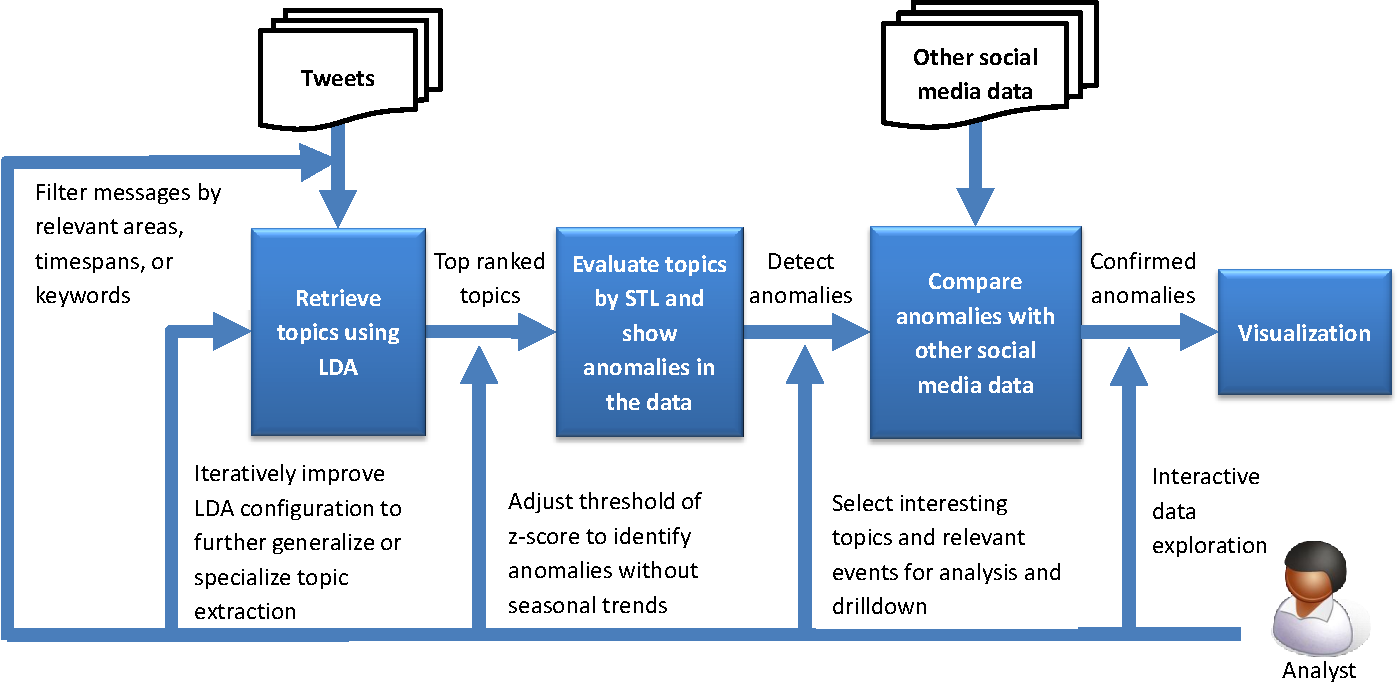
\includegraphics[width=1.0\linewidth]{Overall_Process_crop.pdf}
	\caption{Overview of our iterative analysis scheme for event detection and examination.}
	\label{fig:ad_process}
\end{figure}


\subsection{Social Media Retrieval and Analysis System}
\label{subsec:analysis_system}
Our modular analysis workbench ScatterBlogs was already featured in previous works \cite{Bosch:2011:SGD,Thom:2012:SAD}. 
It proved itself very useful for fundamental tasks like collection, exploration and examination of individual, as well as aggregated, social media messages. The UI of the system is composed of several interconnected views and the main view houses a zoomable openstreetmaps implementation showing message geolocations on a world map. The system features a text search engine and visual content selection tools that can be used to retrieve messages, show spatial and temporal distributions and display textual message contents. Additional visualizations and map overlays provide the analyst with powerful inspection tools, such as a kernel-density heatmap similar to \cite{Maciejewski:2010:VAA}, to show aggregated and normalized message distributions and a movable lens-like exploration tool (called \textquoteleft content lens\textquoteright) that aggregates keyterm frequencies in selected map areas \cite{Bosch:2011:SGD}. To indicate spatiotemporal anomalies in the message set, the system features a mechanism to detect spatiotemporal clusters of similar term usage, and suspicious message clusters can be represented as Tag Clouds on the map \cite{Thom:2012:SAD}. For the real-time collection of messages using the Twitter Streaming API the system features a scalable extraction and preprocessing component. This component was used to collect Twitter messages since August 2011 and it currently processes up to 20 Million messages per day, including the almost complete volume of up to 4 million messages that come with precise geolocation information.

\subsection{Visual Topic Exploration and Event Evaluation}
Results from the topic retrieval and event detection as described in Section~\ref{sec:social_analytics} can be iteratively refined by means of visual result presentation and interactive parameter steering. Both, the final result of event detection as well as intermediary findings during data filtering and topic extraction can be used by the analyst to adjust the process in order to identify interesting topics and keyterms as well as relevant map areas and timespans for a given analysis task. New insights can be generated on each of four individual analysis layers which, in conclusion form an iterative analysis loop from data filtering to result visualization:
\begin{itemize}
	\item \textbf{Spatiotemporal Data Filtering:} The analyst selects an initial spatiotemporal context of Twitter messages to be represented in the visualization and to serve as a basis for analysis. 
He can do so by using textual as well as spatiotemporal query and filter mechanisms that load the relevant base message set from a larger database into active memory. 
The analyst can further filter the base set and remove unimportant parts by using a time-slider, depicting temporal message densities, or polygon and brush selection tools.
% shortened because is prior art
%To filter this base set and to remove unimportant parts, the analyst is provided with an hierarchical time-slider, allowing individual selection of days, hours and minutes. 
%This slider also shows message densities as histograms along the three temporal axis in order to identify high message concentrations. 
%At the same time, polygon and brush selection tools can be applied for spatial filtering.
Using these tools the analyst can gain an initial impression of the spatial and temporal distribution and location of messages that could be relevant for his analysis task.
	\item \textbf{LDA Topic Examination:} In the subsequent step the analyst can choose to start the topic extraction either on the whole analysis context or on some subset of selected messages. At this stage he can utilize the configuration parameters of LDA extraction to interactively explore available topics by generalization and specialization. In this regard the most important parameter is the number of topics that have to be defined for the topic model inference. If the analyst decreases the number using the provided tools, the extracted topics will be more general. If he increases it, they will be more specific and thus candidates for small but possible important events. Once topics are generated from the data they will be presented to the analyst through a list of small tag clouds for each topic. He can now select the topics from the list to see their individual message distribution on the map and the temporal distribution in the time-slider. 
	\item \textbf{STL Evaluation:} Depending on the analyst's choice, the topics can be evaluated and ordered based either on absolute topic frequency or based on abnormality estimates that have been computed using STL. As described in Section~\ref{subsec:filtering}, a valid estimate of abnormality depends on the computation of z-scores from data seven days prior to the observed time frame. Therefore, the STL evaluation will extend the data examination to a range prior to the selected spatiotemporal context, if data is available. Once abnormality is computed for each topic, the topic list will be ordered according to the values and the topics with most outstanding abnormality are highlighted.
	\item \textbf{Crosscheck Validation:} Each selection of messages is accompanied by charts showing the total time series and the remainder components for the selected message set using STL. This is true for spatiotemporal selections as well as for selections using the LDA topic list. In addition to the geolocated Twitter messages this STL is at the same time performed for data that has been extracted from supplemental services like Flickr and YouTube. Based on the multiple charts the analyst can crosscheck the importance and abnormality of examined events and topics.
\end{itemize}


In our system, the analyst is supposed to iteratively use these means of semi-automated processing, visualization and interaction to refine the selection of messages up to a point where he can begin to examine individual message details.
For this task, he can then utilize tools like the content lens for small scale aggregation or the table view to read the messages textual content.
The application of these tools is shown in Figure~\ref{fig:tagcloud}. Usually the most valuable messages will be reports from local eyewitnesses of an important event or from insiders for a given topic. Thus, to retrieve large quantities of such messages helping to understand an ongoing event or situation will be the final goal of the iterative process. Unusual topics, suspicious keyword distributions and events with high STL abnormality discovered on the repeatedly traversed analysis layers can guide the analysis from a very broad and general overview to very specific topics and a relatively small message set suitable for detailed examination.

\begin{figure}[htb]
	\centering
	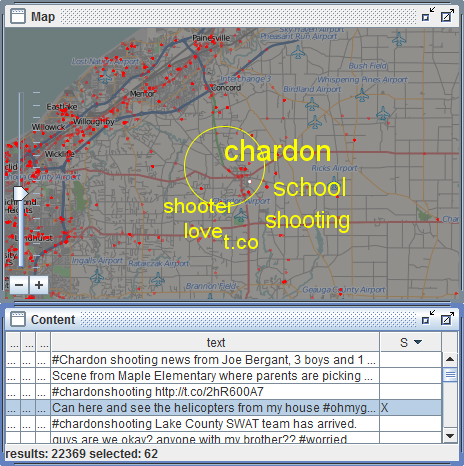
\includegraphics[width=0.6\linewidth]{images/content_investigation}
	\caption{Examining the location of the Chardon high school shooting with a text aggregating content lens.}
	\label{fig:tagcloud}
\end{figure}

\section{Case Study}
\label{sec:case_study}
In this section, we present three case studies for our system covering different types of events including the Chardon High School Shooting, 
the Occupy Wall Street protests in New York, and the 2011 Virginia Earthquake. 
The first case shows how analysts can use our system efficiently to find and explore an abnormal event.
The second case highlights the differences between social media types by cross validation of a planned event.
Finally, the last example showcases the effects of an abrupt, unexpected, natural disaster.

%\begin{figure*}[t]
	%\centering
	%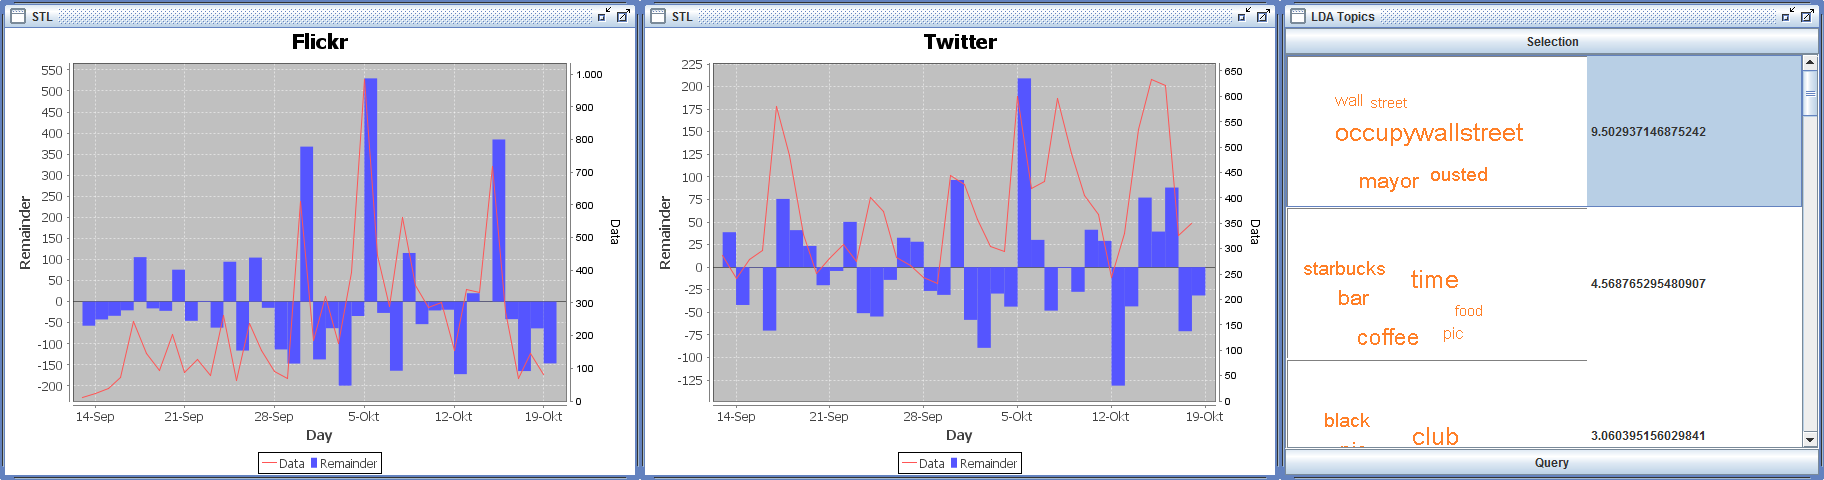
\includegraphics[width=1.00\linewidth]{images/flickrtwitter}
	%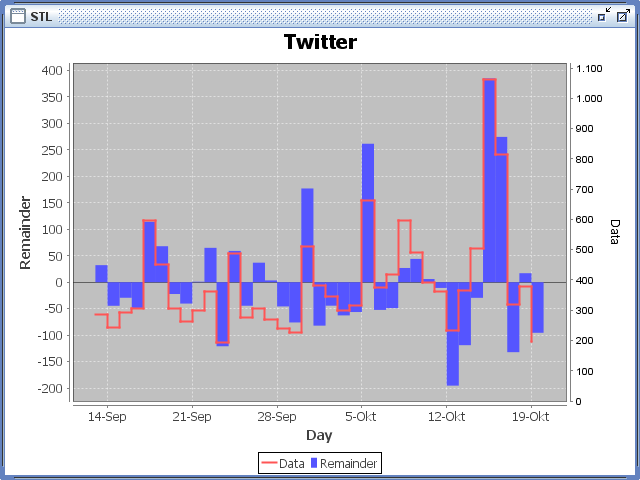
\includegraphics[width=0.45\linewidth]{images/twitter_wallstreet.png}
	%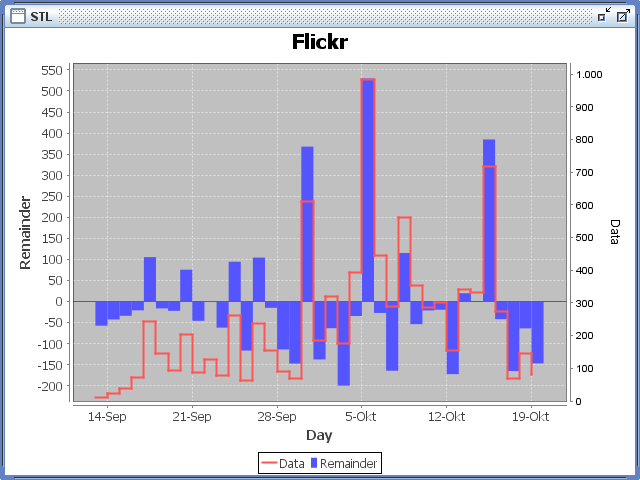
\includegraphics[width=0.45\linewidth]{images/flickr_wallstreet.png}
	%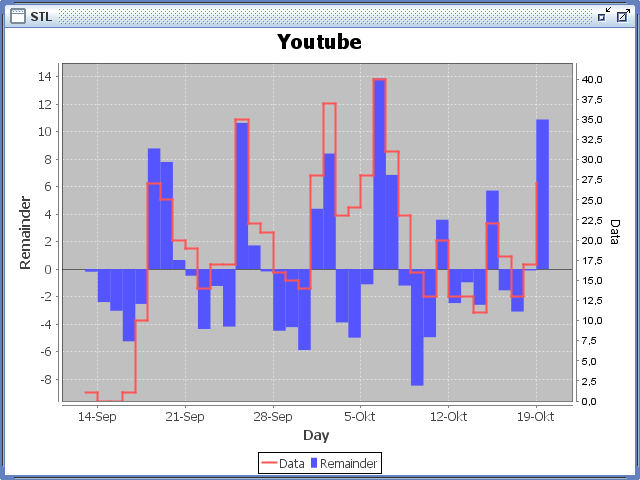
\includegraphics[width=0.45\linewidth]{images/occupyyoutube.png}
	%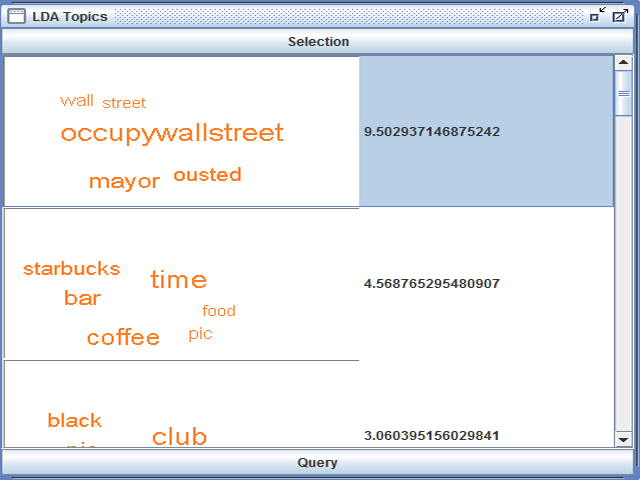
\includegraphics[width=0.45\linewidth]{images/tags_wallstreet.png}
	%\caption{Cross validation of an event using Twitter, Flickr, and YouTube data for the Occupy Wall Street Protests.
	%The protests occurred on Sep. 17 and 30, Oct. 5 and 15. The extracted topics from messages using LDA are displayed with the z-score
	%on the right. The line charts show the remainder components $R_{t}$ (blue) and the original data volumes $Y_{t}=ts_i$ (red) for the STL evaluation.}
	%\label{fig:wallstreet}
%\end{figure*}
	

\subsection{Ohio High School Shooting}
\label{subsec:ohio_shooting}
On February 27, 2012, a student opened fire inside the Chardon High School cafeteria in the early morning.
The gunman killed one student and injured four, from which two eventually died after the incident.

To examine this incident we first locate and select the broader Cleveland area on the map and select a time frame covering three days from February 26 to February 28. 
Using the text search engine and a wildcard query (\textquoteleft *\textquoteright) we can establish an exploration context showing all messages plotted on the map with their respective contents and meta data listed in a separate table view. First, we want to get a broad overview of the topics discussed in the region and thus we select all messages in the area and apply the LDA extraction tool to the current selection. In order to see the most general topics, we chose a low parameter value for the number of topics and a high iteration count to achieve good separation. At this level of semantic detail, the extracted topics indicate messages about the NBA all-star game (February 26 in Orlando) with keywords like \textit{kobe, game, dunk and lebron} as well as the showing of the movie \textquoteleft The Lion King\textquoteright on TV with keywords \textit{king, lion, tv}. If we look at the STL-Diagrams of these topics and the computed z-scores, we also see a peak for these events. By clicking on the retrieved topic representations the associated messages are highlighted in each view. By reading some of the message contents (e.g. \textit{'Watching my fav. Movie on ABC family..... Lion King!!!!', 'Can't wait till the dunk contest starts!'}), the analyst can easily disqualify these from further analysis.

To get a higher semantic resolution we can now increase the number of topics and slightly decrease the iteration count in order to achieve a fast computation. By selecting 20 topics, the topic indicating the shooting event is extracted and indicated by keyterms like \textit{shooting, chardon and school}, alongside the other topics. Although the proportion of the topic is not very high compared to the others, the topic receives a very high z-score (i.e., 3.77) and is ranked among the top five topics (highlighted in orange). Figure~\ref{fig:system} demonstrates the system view of this observation. An analyst can now select the incident topic to see the spatial distribution of associated messages on the maps as well as the temporal distribution in the timeslider histogram. By examining messages using the content lens to aggregate topics over map areas as well as the tools for reading individual message contents, we can easily distinguish between messages informed by media reaction and messages of actual observers in the Chardon High School area. In this case, after isolating the messages from local observers, we find messages like \textit{\textquoteleft Omg shooting at Chardon High School?!?!\textquoteright} and \textit{\textquoteleft Helicopter overhead. We are on scene. Message from school says students moved to middle school\textquoteright}.

\begin{figure}[tb]
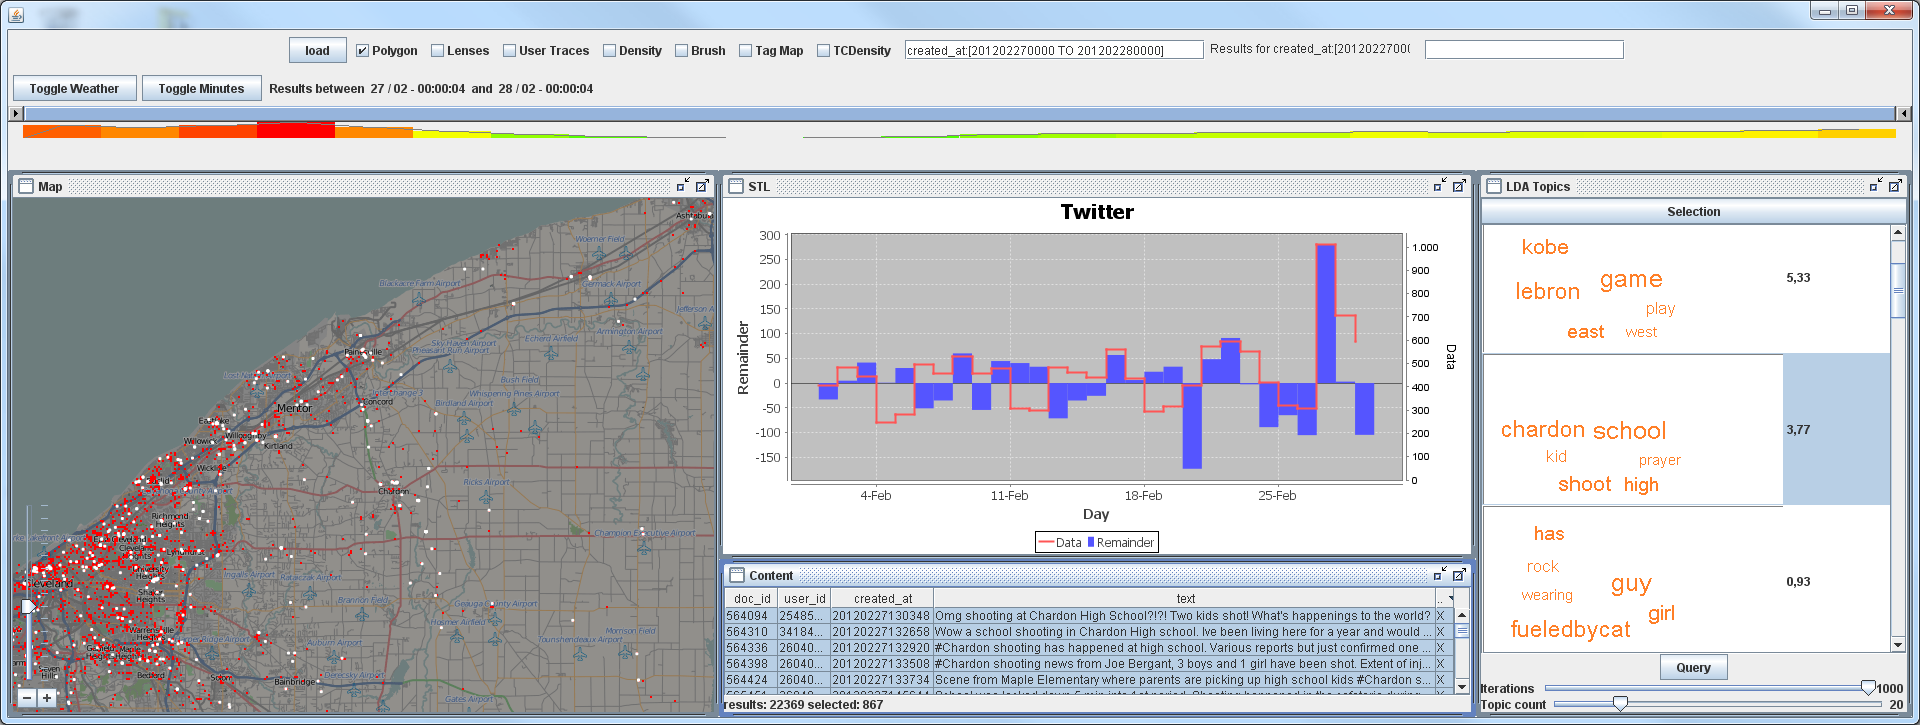
\includegraphics[width=1.0\linewidth]{teaser}
\caption{Social media analysis system including message plots on a map, abnormality estimation charts and tables for message content and topic exploration. 
  It can be seen, how the Ohio High School Shooing on February 27, 2012 is examined using the system. The selected messages, marked as white dots on the map, show retrieved Tweets that are related to the event.}
\label{fig:system}
\end{figure}



%To discussion -> Athough the detected messages could help to identify local witnesses of some event, the frequencies of messages with geocoordinates are still very low in moderately populated areas ---- daher könnte man die Nützlichkeit zum gegenwärtigen Zeitpunkt sicher hinterfragen...

%\footnote{\url{http://www.cbsnews.com/8301-504083_162-57386775-504083/third-chardon-high-school-shooting-victim-demetrius-hewlin-dies/}}

\subsection{Occupy Wall Sreet}
\label{subsec:occupy_wallst}

Starting on September 17, 2011 in the Wall Street financial district in New York City,
people have been gathering for the Occupy Wall Street protest movement.
The movement against economic inequality has since spread to other major cities throughout the world.
Various social media services including Twitter, Facebook, Flickr and Youtube have been utilized both by the participants and the global media for communication and reports about the movement in forms of text, images and videos. 
For the related extracted topic (\textit{occupywallstreet, wall, takewallstreet, takewallst, park}), 
Figure~\ref{fig:wallstreet} shows the results of our abnormality estimation for the three social media services Twitter, Flickr, and YouTube over the course of one month.
As shown in Figure~\ref{fig:plot}, in each of the marked regions, at least two of the services show z-scores over 2.0 and they correspond to actual events during the Occupy Wall Street protests.
From this experimental result, one can derive a strong correlation between the three social media data sources.
The related data volumes and remainder ($R$) are shown in Figure~\ref{fig:wallstreet} for all three providers.

\begin{figure}[tb]
\centering
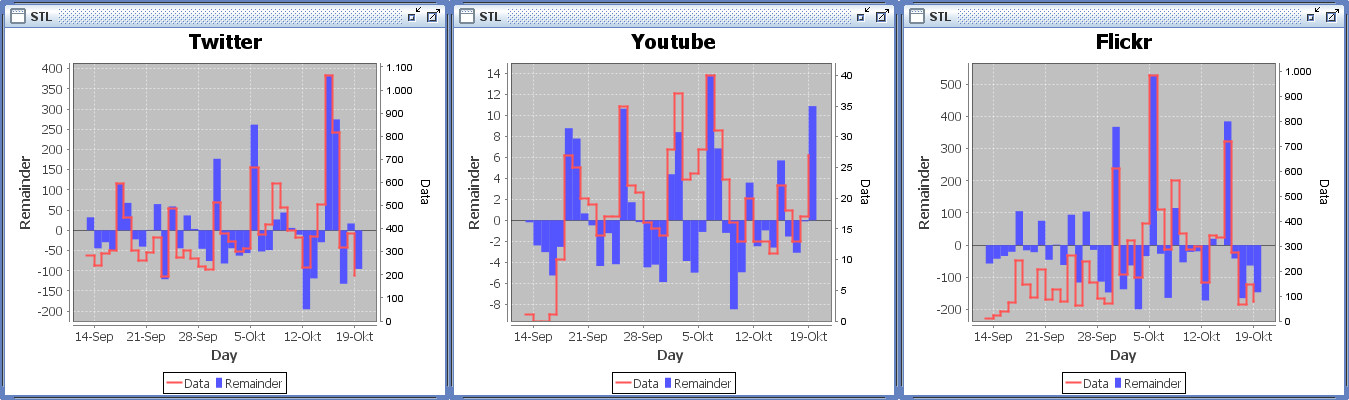
\includegraphics[width=1.0\linewidth]{crosscompare_new}
\caption{Cross validation of an event using Twitter, Flickr, and YouTube data for the Occupy Wall Street Protests.
	The protests occurred on Sep. 17 and 30, Oct. 5 and 15. The line charts show the remainder components $R$ (blue) and the original data volumes $Y$ (red) for the STL evaluation. The scales on the right and left side of each chart view are adapted to the maximum values.}
\label{fig:wallstreet}
\end{figure}


\begin{figure}[tb]
\centering
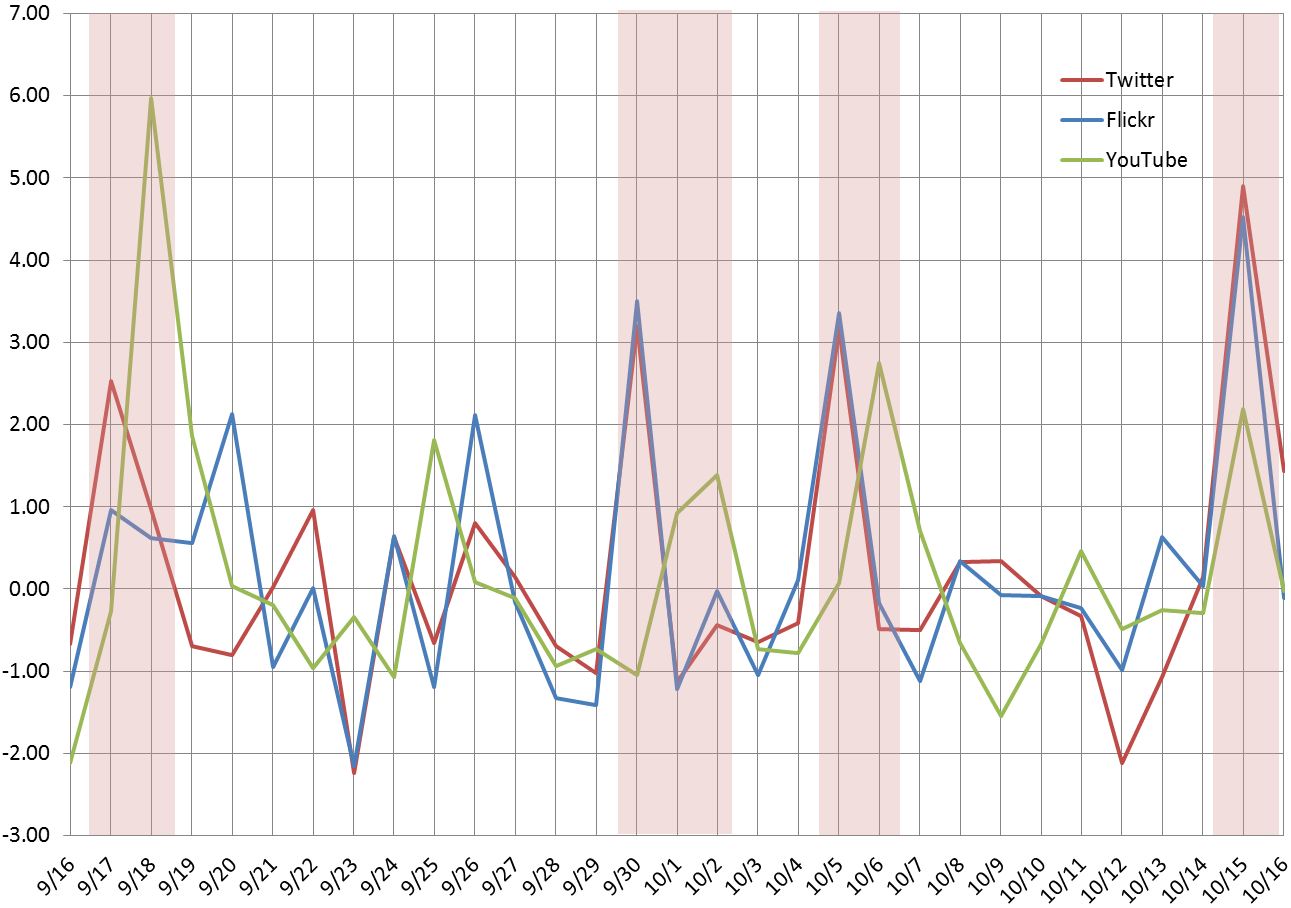
\includegraphics[width=0.8\linewidth]{z-score-plot}
\caption{Abnormality and correlation on multiple social media sources. 
As a result of high z-scores around the same time periods, we found a strong correlation 
between the three social media sources. Marked regions correspond to periods where at least 2 providers received scores over 2.0.}
\label{fig:plot}
\end{figure}



As shown in Figure~\ref{fig:plot}, on September 17 (the first day of the protests with approximately 1,000 participants~\cite{Sept17}),
only the Twitter stream received an abnormal score while the Flickr and YouTube data artifacts are delayed by 1-3 days.
We attribute this initial delay to the simple nature of Twitter usage compared to Flickr and YouTube where the data potentially has to be recorded, edited, and uploaded and is thus more labor intensive.
Additionally, eighty protesters where arrested while marching uptown on September 24, but even though Flickr and YouTube reaction on this event created higher z-scores in the following days, they were not significant enough to register an event.
The following spikes of high z-scores overlap with a march across the Brooklyn Bridge (Oct. 1~\cite{Oct01}), a large demonstration (Oct. 5~\cite{Oct05}), and globally coordinated protests (Oct. 15~\cite{Oct15}).

%For YouTube, the high abnormalities usually come with a delay between one and two days.
%Our system found the additional abnormal events \textit{oakland, tear, gas, general, san}~\cite{Duell:2011:OOI} and \textsl{bridge, brooklyn, arrests, march, police}~\cite{Chiaramonte:2011:CMO} in the YouTube meta-data, which were not detectable in Twitter and Flickr.
%Our system also provides further analysis on YouTube data. 
%We applied our abnormality estimation method to meta-data from YouTube. 
%Our system additional found more abnormal events;

%%
%% Table of experimental results of topic model
%%
%\begin{table}\footnotesize
%\begin{table}
%\small
%\centering
%\begin{tabular}{|l|c|c|c|}
%	\hline
%	 Date & Twitter & Flickr & YouTube \\
%	\hline\hline
%%	Sep. 16, 2011 & -0.67 & -1.19 & -2.12 \\
%	Sep. 17, 2011 & \textbf{2.53} & \textbf{0.97}& \textbf{-0.26} \\ %& The protests movement began \\
%	Sep. 18, 2011 & 0.97 & 0.62 & 5.98 \\ 
%	Sep. 19, 2011 & -0.69 & 0.56 & 1.86 \\
%	Sep. 20, 2011 & -0.80 & 2.13 & 0.04 \\
%	Sep. 21, 2011 & 0.02 & -0.95 & -0.19 \\
%	Sep. 22, 2011 & 0.96 & 0.01 & -0.96 \\ 
%	Sep. 23, 2011 & -2.24 & -2.15 & -0.34 \\
%	Sep. 24, 2011 & 0.63 & 0.64 & -1.07 \\
%	Sep. 25, 2011 & -0.66 & -1.19 & 1.81 \\
%	Sep. 26, 2011 & 0.80 & 2.11 & 0.08 \\
%	Sep. 27, 2011 & 0.14 & -0.16 & -0.11 \\
%	Sep. 28, 2011 & -0.70 & -1.32 & -0.94 \\
%	Sep. 29, 2011 & -1.02 & -1.41 & -0.73 \\
%	Sep. 30, 2011 & \textbf{3.20} & \textbf{3.50} & -1.05 \\%& Big movement \\
%	Oct. 1, 2011 & -1.14 & -1.22 & 0.92 \\
%	Oct. 2, 2011 & -0.44 & -0.03 & \textbf{1.38} \\
%	Oct. 3, 2011 & -0.64 & -1.05 & -0.73 \\
%	Oct. 4, 2011 & -0.42 & 0.11 & -0.77 \\
%	Oct. 5, 2011 & \textbf{3.17} & \textbf{3.36} & 0.07 \\ %& Unions, students join the protest\\
%	Oct. 6, 2011 & -0.49 & -0.18 & \textbf{2.75} \\
%	Oct. 7, 2011 & -0.50 & -1.12 & 0.7 \\
%	Oct. 8, 2011 & 0.32	& 0.34 & -0.65 \\
%	Oct. 9, 2011 & 0.34	& -0.07 & -1.54 \\
%	Oct. 10, 2011 & -0.09 & -0.08 & -0.67 \\
%	Oct. 11, 2011 & -0.33 & -0.23 & -0.46 \\
%	Oct. 12, 2011 & -2.12 & -0.99 & -0.49 \\
%	Oct. 13, 2011 & -1.07 & 0.63 & -0.26 \\
%	Oct. 14, 2011 & 0.15 & 0.04 & -0.3 \\
%	Oct. 15, 2011 & \textbf{4.90} & \textbf{4.53} & \textbf{2.19} \\ %& Global day of action \\
%%	Sep. 17, 2011 & 2.53 & 0.97 & Sep. 18, 2011 & 5.98 \\ %& The protests movement began \\
%%	Sep. 30, 2011 & 3.20 & 3.50 & Oct. 2, 2011 & 1.38 \\%& Big movement \\
%%	Oct. 5, 2011 	 & 3.17	& 3.36 & Oct. 6, 2011 & 2.75 \\ %& Unions, students join the protest\\
%%	Oct. 15, 2011   & 4.90 & 4.53 & Oct. 15, 2011 & 2.19 \\ %& Global day of action \\
%	\hline
%\end{tabular}
%\caption{Abnormality and correlation on multiple social media. 
%As a result of the high z-scores around the same time, we found a strong correlation 
%between the three social media sources.}
%\label{T:Correlation}
%\end{table}
%\footnote{\url{http://www.nytimes.com/2011/11/25/business/media/occupy-movement-focuses-on-staying-current-on-social-networks.html}}

%\subsection{2011 Virginia earthquake}
%\label{subsec:virginia_earthquake}
%A magnitude 5.8 earthquake occurred on August 23 afternoon, 2011 in Mineral, Virginia,
%according to the U.S. Geological Survey\footnote{\url{http://earthquake.usgs.gov/earthquakes/recenteqsww/Quakes/se082311a.php}}.
%During and after the tremors were felt along the East Coast,
%Twitter users posted more than 40,000 earthquake-related reaction tweets
%within a minute of its occurrence\footnote{\url{http://mashable.com/2011/08/23/virginia-earthquake/}}.
%There are some example Twitter messages;
%\textit{EARTHQUAKE!!!!!!!}; \textit{Whoa!!!! Just experienced an earthquake here in Virginia!!!!}; 
%\textit{Omg I just felt an earthquake}.
%Using our method, we found also the z-score of the topic indicating the earthquake event was 
%extremely high (i.e., 10.63).
\subsection{2011 Virginia Earthquake}
\label{subsec:virginia_earthquake}
For the last use case we examine a magnitude 5.8 earthquake that occurred on the afternoon of August 23rd 2011 in Mineral, Virginia~\cite{USGS:2011:M5V}.
%\footnote{\url{http://earthquake.usgs.gov/earthquakes/recenteqsww/Quakes/se082311a.php}}.
Starting with the minute of the earthquakes occurrence, Twitter users posted more than 40.000 earthquake-related Tweets reporting tremors they felt along the East Coast~\cite{Indvik:2011:ECT}.
%\footnote{\url{http://mashable.com/2011/08/23/virginia-earthquake/}}.
Among these were messages like:
\textit{\textquoteleft EARTHQUAKE!!!!!!!\textquoteright}; \textit{\textquoteleft Whoa!!!! Just experienced an earthquake here in Virginia!!!!\textquoteright}; and 
\textit{\textquoteleft Omg I just felt an earthquake\textquoteright}.
Figure~\ref{fig:earthquake} gives an impression how our system is applied to examine this event.

\begin{figure}[htb]
	\centering
	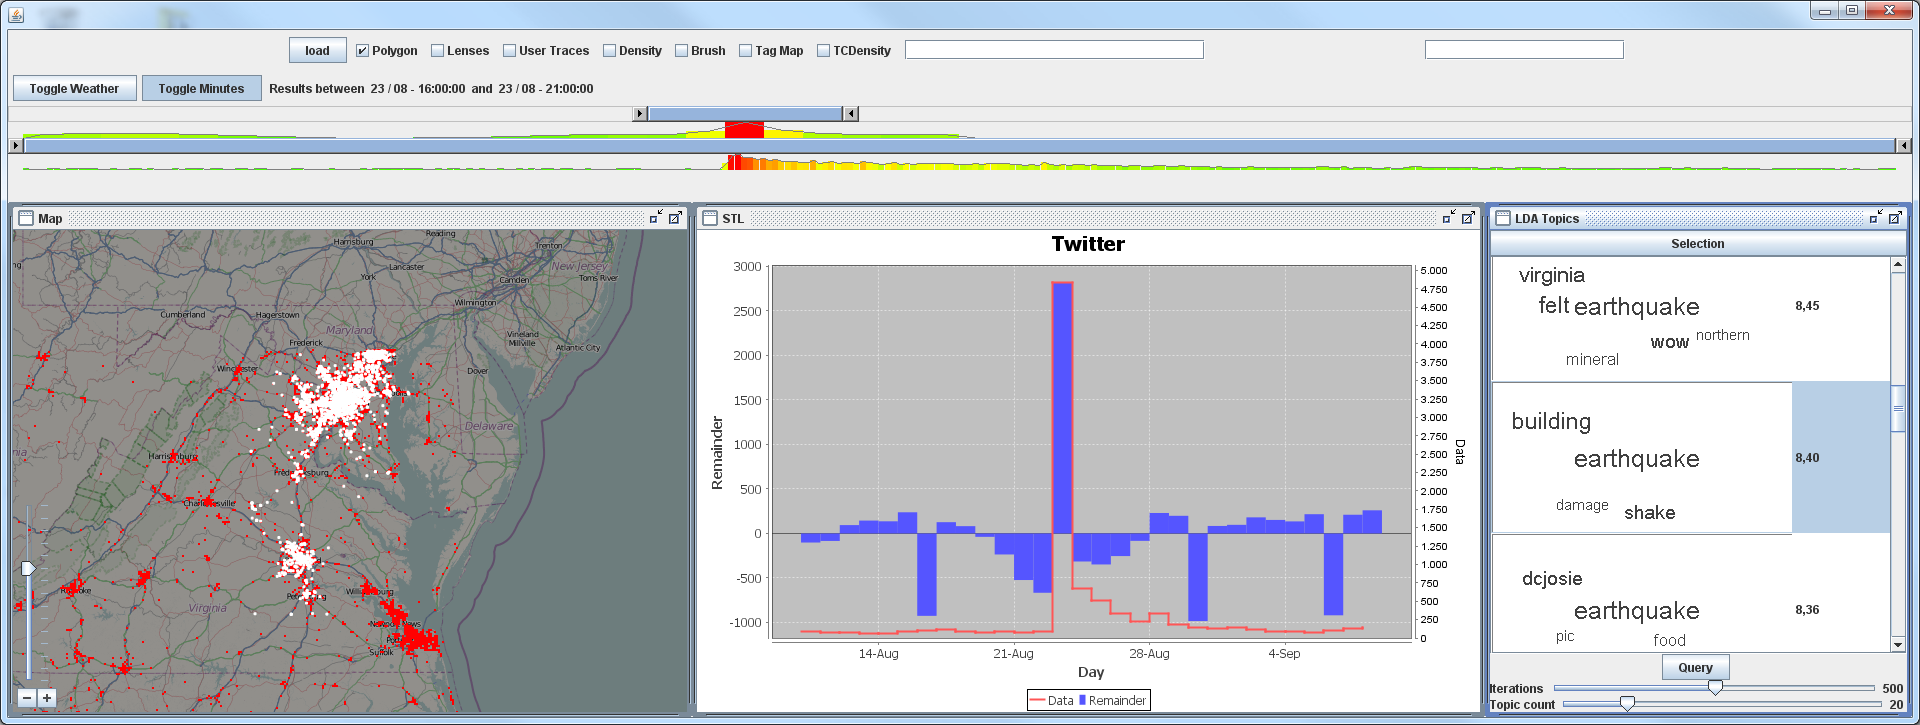
\includegraphics[width=1.0\linewidth]{earthquake3}
	\caption{Virginia earthquake on August 23rd, 2011. Our abnormal event detection system detects the earthquake event
	using our STL based anomaly detection algorithm. The abnormality degree is extremely high
	on August 23rd, 2011 (times are given in UTC).}
	\label{fig:earthquake}
\end{figure}

For the analysis we begin with selecting the Virginia area from Baltimore to Virginia Beach and three days around the 23th. A topic extraction with 5 topics and just 100 iterations already retrieves two earthquake related topics showing that this event is very prominent within the selection. By clicking these topics one can observe that the highest density of earthquake messages can be found in the Washington, Baltimore and Richmond areas. 

To observe the areas in more detail we combine the topic selection with a spatial selection of the three cities and reapply the topic extraction. This time we use 20 topics with 500 iterations. Since we are now operating only on earthquake related messages, the retrieved topics all contain earthquake as a dominant keyword. On this level of detail we can see topics indicating that buildings have been evacuated due to the earthquake (\textit{earthquake, people, evacuated, early, building}) and that damage has been caused (\textit{earthquake, building, shake, damage}). The z-scores for all top ranked topics are now very high (often above 8.0) and thus indicate the high abnormality of this event. 

Finally, when going into even higher detail with 100 topics and 1000 iterations we can see smaller events within the big earthquake event. For example, one topic indicates that damage was caused to the Washington Monument and by clicking on the topic we can see messages like \textit{\textquoteleft damage to Washington Monument\textquoteright}; \textit{\textquoteleft Washington Monument is tilting?!? \textquoteright}; and \textit{\textquoteleft Helicopter just landed next to Washington Moniment, west side. \#DCearthquake \textquoteright}. There are also misleading messages, indicating that the damage to the Washington Monument was just false rumors: \textit{\textquoteleft the Washington monument was not damaged in any way from the earthquake. \#rumor\textquoteright}. However, media crosschecks show that visible damages did in fact happen and will probably cost the city 15 million dollars to repair~\cite{Huffingtonpost:2012:Web}.

At this point, it is important to note, that while several earthquake topics produced significant z-values in Twitter, the event did not produce high z-scores in Flickr and YouTube.
This is probably due to fact, that many people will write a quick message after a shock has been felt by themselves, but it takes quite some time until images or videos are uploaded from cameras to Flickr and YouTube. The event also demonstrates that large and unexpected events will produce immediate and significant reactions in services like Twitter and they can thus easily be detected by using our system.

\section{Discussion}
\label{sec:disc}
In this section we want to discuss four important notes and observations relevant to the presented approach.

\textbf{Event Types:} As was demonstrated with the three case studies, events in social media can be categorized into two different types. 
The 2011 Virginia Earthquake and the Ohio High School Shooting can be categorized as abrupt or disaster events,
while Occupy Wall Street can be considered a social and planned event.
The two types of events have quite distinguishable features.
For the abrupt events, there is a strong change in daily counts mainly in the text based Twitter messages.
For the planned event, the Twitter signal may still be faster, but due to the gradual increase and decrease, it is less pronounced.
In contrast, Flickr and YouTube have delayed, but very prominent changes, for planned events; 
however, we could not find significant signals for abrupt events.
This reflects that video and photo recording happen rarely during abrupt events.
Social events, e.g., Occupy Wall Street or election debates, however, have a high impact on such multimedia based social media; 
Relevant videos, photos, and even meta-data (e.g., descriptions, tags) allow analysts to find additional information about them.
We, therefore, think that cross validating events among multiple social media types is important in order to establish situational awareness.

\textbf{Base Data:} Regarding the base data, it is important to note, that our approach depends on geo-located Twitter messages with precise coordinates, which are only a fraction of the whole Twitter stream.
While this fraction still consists of several million messages per day, 
it is not a representative sample of the population, because it mainly covers mobile users equipped with GPS enabled devices.
We think, however, that mobile users, who share their daily experiences freely, are the most relevant group for situational awareness scenarios.
Some studies~\cite{Cheng:2010:YYT, Jalal:2012:WIT} tried to overcome the problem of location information scarcity in Twitter messages, which adds another source of uncertainty.
First, the user's self reported locations can be outdated.
Second, the geo-coding of the location can be considerably wrong due to place name ambiguities.
Furthermore, we have just shown the feasibility of the approach for Twitter, Flickr, and YouTube data, but it can easily be adapted to other social media providers like Facebook or Forsquare as well, in order to widen the sample of the population.

\textbf{Probabilistic Models:} In this work, we use STL to decompose time series of topic streams.
There are many alternative statistical models for this task, such as DHR (Dynamic Harmonics Regression)~\cite{Young:1999:DHR} and SARIMA (Seasonal AutoRegressive Intergrated Moving Average)~\cite{Box:1990:TSA}.
DHR and SARIMA models are particularly useful for forecasting and STL can also be used for prediction based on seasonal (periodic) time series~\cite{Jiang:2010:MML}.
Our main reasons for choosing STL was the fact that it is non-parametric, can be computed faster than SARIMA~\cite{Jiang:2010:MML} and needs less training data for equally good results.

\textbf{End User Feedback:} We requested informal feedback from users within our institutes and received comments and suggestions. 
To compare the LDA topic modeling plus the seasonal-decomposition based abnormality analysis versus only the LDA topic modeling, we enabled our system to switch between these modes. 
The users were impressed by the fact that both results (two lists of topics) from two different modes were quite different. 
Highly ranked topics by LDA topic modeling consisted of ordinary words, while the combined analysis was indicating unusual events. 
They noted that the tightly integrated visual analysis workbench was useful to apply the automated methods. 
Furthermore, they suggested a function allowing people to see a pattern of abnormality for a user-defined topic.

\section{Summary}
\label{sec:concl}
We presented an interactive abnormal event detection and examination system for the analysis of multiple social media data sources.
The system uses an abnormality estimation scheme based on probabilistic topic modeling and seasonal-trend decomposition to find and examine relevant message subsets. This scheme is tightly integrated into an highly interactive visual analytics system, which supplements tools based on automated message evaluation with sophisticated means for parameter steering, filtering and aggregated result set exploration.
Three use cases demonstrated the visualization and user interaction within the system and its capabilities to detect and examine several different event types from social media data.
The ability to crosscheck findings based on three distinct social media sources revealed the kinds of correlations that can be expected from various event types.
%Finally, we showed that our interactive system allows an effective analysis of a massive social media data set.

%For future work, we will further investigate context-based analysis and improve the current detection algorithm to allow for a faster analysis.
%Due to the fast-paced and low quality nature of microblogging, we will also investigate the effects of additional preprocessing options like automated spell-checking or synonym recognition under the constraint of preventing ambiguities.
%Furthermore, we want to supplement the system with real-time monitoring features, demanding additional means for adaptive attention guiding as well as interaction techniques for use in high pressure environments. For the final system we are currently preparing a thorough evaluation to test it in cooperation with crisis management personnel and other domain experts.



\chapter{Visual Analytics of Microblog Data for Public Behavior Analysis in Disaster Events}

%\textit{Hurricane Sandy} approached Northeastern United States during late October 2012 and New York City announced a mandatory evacuation of some low-lying areas in the morning on October 28th. these three figures show the southern part of Manhattan. (Left) shows spatial user-based Tweet distribution from noon to 4:00 PM, right after the evacuation order. We overlay the locations of big supermarkets (blue pin) on the same heatmap. we see relatively many number of people immediately go to supermarkets. (Center and Right) shows the distributions during one and two weeks before the same time period. The hotspots are locationally much different from ones of (Left). The green pins on the maps, (Center and Right) indicate the locations of big parks in the southern region of Manhattan. The many hotspots overlap with the park areas; this would be a normal situation on Sunday.


%For emergency and disaster management, analysis of public behavior, such as how people prepare and respond to disasters, is important for evacuation planning.
Analysis of public behavior plays an important role in crisis management, disaster response, and evacuation planning. 
As social media has played a pervasive role in the way people think, act, and react to the world (more than 40 million Americans use social media Web sites multiple times a day~\cite{TW:2010:SHF}), social media is changing the way people communicate not only in their daily lives, but also during abnormal events, such as natural disasters.
In emergency situations, people even seek social confirmation before acting in response to a situation, where they interact with others to confirm information and develop a better informed view of the risk~\cite{national:2013:Public}.
A study commissioned by the American Red Cross, found that roughly half of the respondents would mention emergencies and events on their social media channels, and more than two-thirds agree that response agencies should regularly monitor postings on their websites~\cite{ARC:2010:SMD}.
Moreover, a growing number of people are using Location-based Social Network services, such as microblogs, where they create time-stamped, geo-located data and share this information about their immediate surroundings using smart phones with GPS. 
Such spatiotemporal data has great potential for enhancing situational awareness during crisis situations and providing insight into the evolving event, the public response, and potential courses of action. 

%From government agencies and other organizations, to citizens and social platforms themselves, people across the spectrum of social media are leveraging its use to respond to emergencies. 
%According to a 2011 report of the Congressional Research Service, there are two broad categories in the way that we can conceptualize this use of social media: 1) to "somewhat passively" disseminate information and receive user feedback; and 2) to use social media more systematically as an emergency management tool.

%Unfortunately, finding meaningful information for the analysis is challenging and collecting relevant data would create even high cost.

For public behavior analysis in disasters, however, finding meaningful information from social media is challenging. It is almost impossible to perform a straightforward qualitative analysis of the data, since the volume of the data exceeds the boundaries of human evaluation capabilities and normal computing performance.
%since data volume has increased beyond the capabilities of manual evaluations.
Even though we could extract certain information from the data, it is not always easy to determine whether the analysis result of the extracted information is meaningful and helpful.
Thus, there is a need for advanced tools to handle such big data and aid in examining the results in order to understand situations and glean investigative insights.
Given the incomplete, complex, context-dependent information, a human in this analysis and decision-making loop is crucial.
Therefore, a visual analytics approach offers great potential through interactive, scalable, and verifiable techniques, helping analysts to extract, isolate, and examine the results interactively.
In this thesis, we present an interactive visual analytics approach for spatiotemporal microblog data analysis to improve emergency management, disaster preparedness, and evacuation planning~\cite{Chae:2014:Public}.
We demonstrate the ability to identify spatiotemporal differences in patterns between emergency and normal situations, and analyze spatial relationships among spatial distributions of microblog users, locations of multiple types of infrastructure, and severe weather conditions.
Furthermore, we show how both spatiotemporal microblog and disaster event data can help the analysts to understand and examine emergent situations, and evaluate courses of action.
%location-based public behavior and locations of multiple types of infrastructures.


This study is performed using Tweets, as Twitter has been the most popular microblog service in the United States.
We extend our previous work~\cite{Chae:2013:VAM} with additional features of our system and examine their capabilities with several expanded examples in Section~\ref{sec:spatial_decision_support}.
%explain them through more number of case studies (wider range of east coast for the hurricane and a tornado case in the city of Moore) in Section~\ref{sec:spatial_decision_support}.
We also add a discussion section for comparisons and analysis of the case studies.
%that were published before, during, and after 
%hurricane \textquotedblleft Sandy \textquotedblright 
%\textit{Hurricane Sandy}.
%that hit the New York City area on October 29th, 2012.
%For this study, 1,740,114 Tweets published by 92,683 people are used.

Our system evaluates visual analytics of spatiotemporal distribution of Tweets to identify public behavior patterns during natural disasters.
%We propose an approach that visualizes spatiotemporal distribution of Tweets to identify public behavior patterns during natural disasters.
The main features of our approach are as follows:
\begin{itemize}
	\item \textbf{Spatial analysis and decision support:} The system provides effective analysis for exploring and examining the spatial distribution of Twitter users and supporting spatial decision-making using a large volume of geo-located Tweets and multiple types of supplementary information during specific time periods (i.e., disaster events).
\item \textbf{Temporal pattern analysis:} Our visualization system enables the analysts to analyze the temporal distribution of the number of Twitter users posting Tweets in a given location and time.
\item \textbf{Spatiotemporal visualization:} We provide a visualization that allows the analysts to simultaneously analyze both aspects: space and time in a single view.
\end{itemize}

%We first review previous work in Section 2 and describe
%our interactive analysis system in Section 3. 
%We present analysis results for two natural disaster events in Section 4
%and discussion in Section 5. Finally conclusion and future directions are presented
%in Section 6.

\section{Problem Statement and Interactive Analysis Process Design}
\label{sec:analysis_process}
Analysis of public behavior, such as how people prepare and respond to disasters, plays an important role in crisis management, disaster response, and evacuation planning. 
Recently, social media becomes popular and people utilize it for communications not only in their daily lives, but also in abnormal disastrous situations.
Thus, Location-based Social Networks services offer a new opportunity for enhancing situational awareness during disaster events.
Unfortunately, collecting relevant data can be costly and finding meaningful information from the huge volume of social media data is very challenging.
%However, the huge volume of the data is another challenging issue in analyzing and evaluating the data.
Therefore, there is a need for an advanced tool to analyze such massive (\textquotedblleft big\textquotedblright) streaming data and aid in examining the analysis results to better understand situations more efficiently.

\begin{figure}[tb]
%\centering
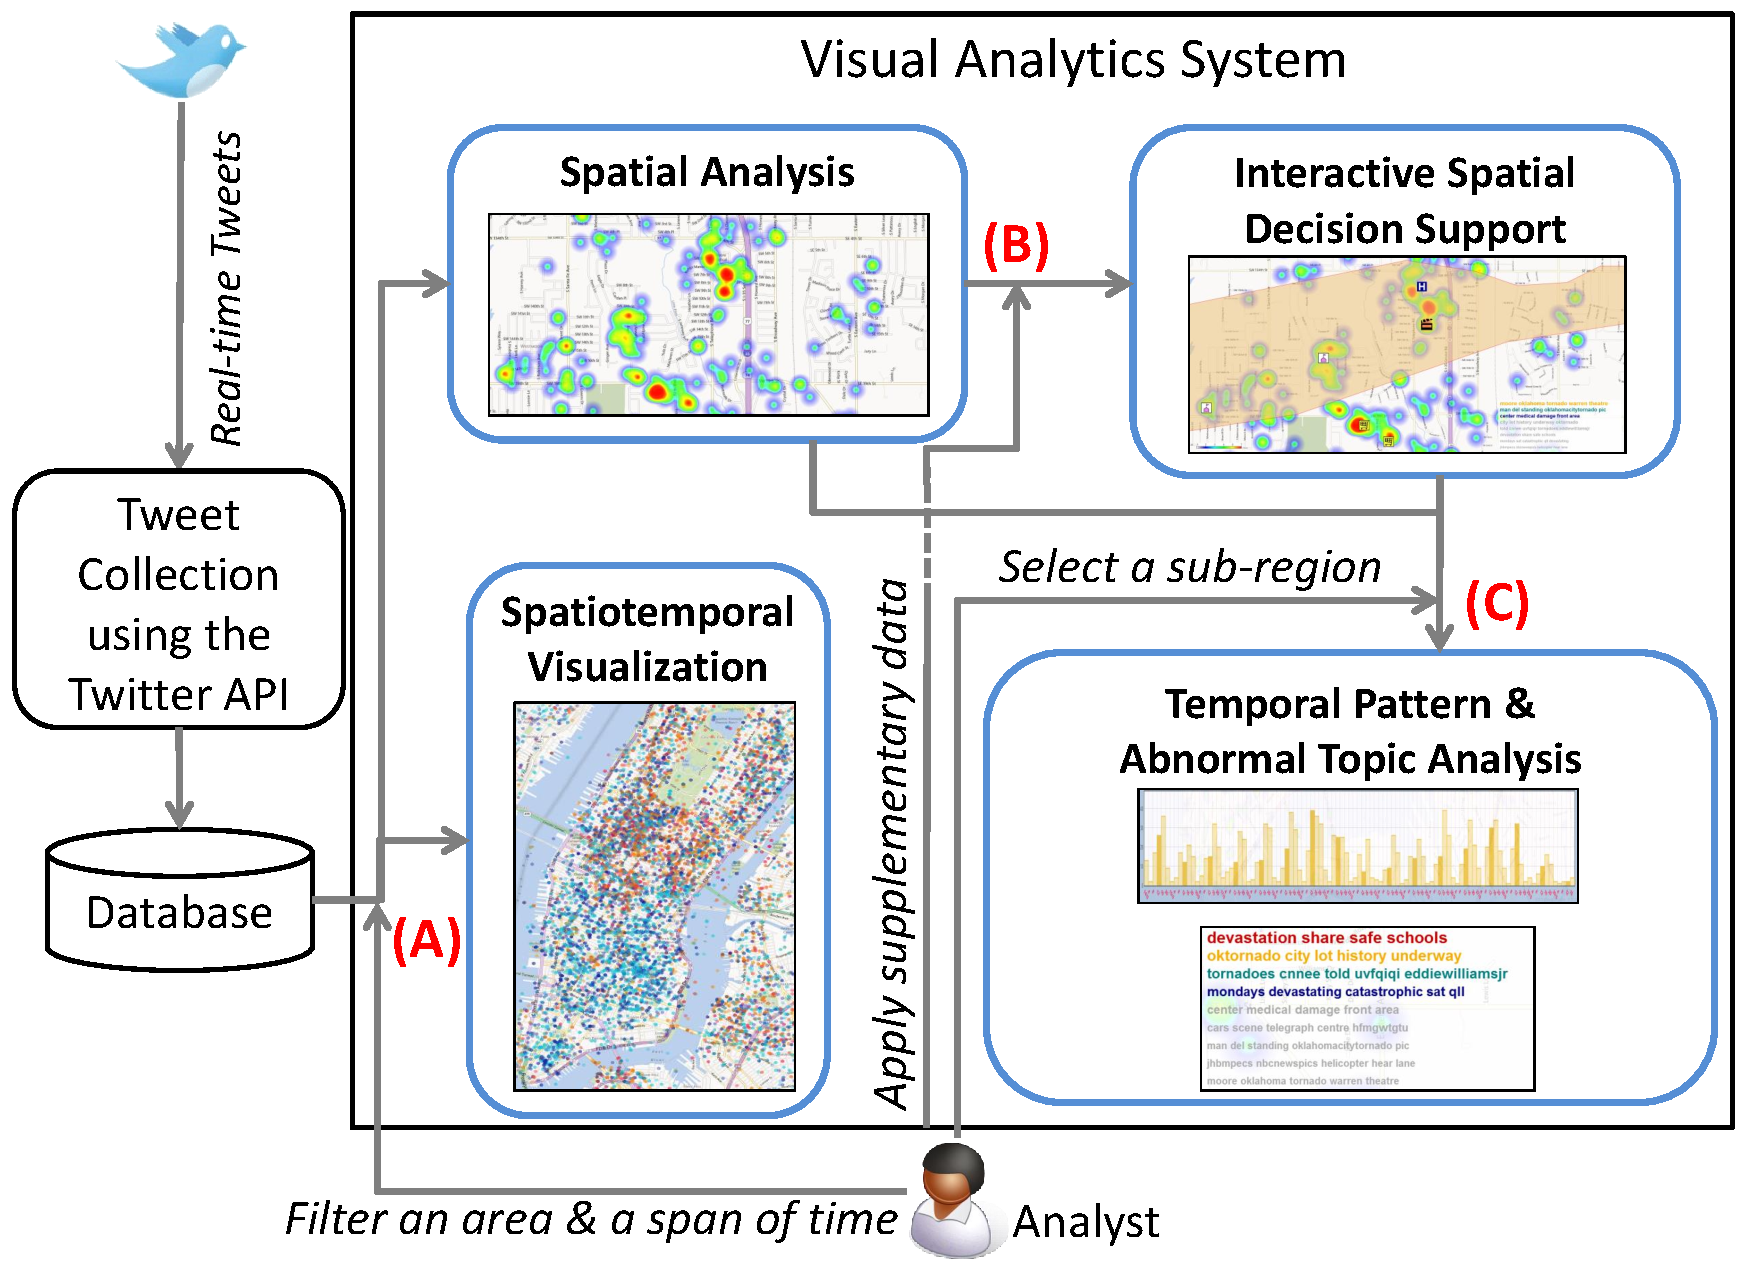
\includegraphics[width=1.0\linewidth]{System_v7}
\caption{Overview of our interactive analysis scheme for public behavior analysis using social media data.}
\label{fig:analysis_process}
%\vspace{-0.4cm}
\end{figure}

Our proposed visual analytics approach provides multiple analysis methods: spatial analysis, spatial decision support, temporal pattern analysis, abnormal topic analysis, and interactive spatiotemporal visualization as shown in Figure~\ref{fig:analysis_process}.
In our system, all methods are tightly integrated based on a user-centered design in order to enhance the ability to analyze huge social media data (Figure~\ref{fig:analysis_process}~(A, B, C)).
Our Tweet collection component obtains real-time Tweets using the Twitter API\textemdash to collect about 2.2 million geotagged Tweets within the United States per day.
In general for spatial analysis, the required accuracy of the geocoordinate depends upon the required level of location granularity.
The data, however, is generated by very reliable GPS and software.
%We can be reasonably certain about their accuracy
We can be reasonably certain about the data accuracy as illustrated in~\cite{TWITTER:2013:GOT}.
For the temporal accuracy of Tweets, we use the time when each Tweet is created. 
Therefore, it is highly accurate if the time setting of the device posting a Tweet is correct.
This large volume of data is stored in our database in order to maintain and track the history of the Twitter stream.
%The analyst can select an area and a timespan to be analyzed.
Our system allows the analysts to query Tweets with a specific area and time span condition (Figure~\ref{fig:analysis_process}~(A)).
%The initially selected spatiotemporal context of Twitter messages is represented by two different analytics components, such as spatial analysis and spatiotemporal visualization.
The initially selected spatiotemporal context of Tweets can be represented by two different analytics components: spatial analysis and spatiotemporal visualization.
Spatial analysis allows the analysts to examine the overall distribution of Twitter users and discover hotspots where relatively more Twitter users post Tweets.
The analysts are able to add supplementary information (infrastructure locations, tornado paths) on top of current information representing outcomes in order to better understand events and increase situational awareness (Figure~\ref{fig:analysis_process}~(B)).
Furthermore, the analysts can select a sub-region within the initial area, so that he can analyze the temporal patterns of the number of Twitter users and extract abnormal topics from the text messages in the selected region (Figure~\ref{fig:analysis_process}~(C)).
In addition, our interactive spatiotemporal visual analytics provides a single view representation for the analysis of both aspects: spatial and temporal characteristics of Tweets at the same time.


\section{Spatiotemporal Analysis}
\label{sec:body}

%Since many social media channels provide time-referenced geographic data, traditional techniques for spatiotemporal zooming and filtering can easily be applied to explore social media data.
%However, as the volume of the data exceed the boundaries of human evaluation capabilities and even normal computing performance, it is almost impossible to perform a straightforward qualitative analysis of the data.
%Therefore, the task for examining and determining whether the extracted result is meaningful is still challenging.
%In order to address the issues, traditional visualization approaches have to be enhanced with more interactive, scalable, and verifiable techniques, helping analysts to extract, isolate, and examine the results interactively.
In this work, we present a visual analytics approach to handle the vast amount of microblog data such as Twitter messages, provide interactive spatiotemporal analysis, and enable the use of multiple types of supplementary spatial infrastructure information for spatial decision support.
%combinational analysis of social media with different types of spatial data 
Analysts select an initial spatiotemporal context of Tweets to be represented in the visualization to serve as a basis for analysis. 
They can also perform the interactive spatiotemporal queries that load the relevant datasets from a larger database.

%in order to examine and verify the results.
%For the public behavior analysis in disasters, however, finding meaningful information from social media is challenging, since data volumes have increased beyond the capabilities of manual evaluation.
%Even though we extract certain information from the data set, it is not always easy to determine whether the result is meaningful.
%Thus, there is a need for advanced tools to handle such big data and even aid in examining the results in order to understand the situations and glean investigative insights.
%In this paper, we present an interactive visual analytics tool for spatiotemporal social media data analysis to improve emergency management, disaster preparedness and evacuation planning by allowing to identify spatiotemporal differences between emergency and normal situations, and analyze spatial relationship between location-based public behavior and locations of multiple types of infrastructures.




\subsection{Spatial Analysis}
\label{sec:spatial_analysis}
%
Social media embedding geo-location information into the data is extremely useful in analyzing location-based public behaviors.
Such spatial analysis, therefore, is important in order to manage and prepare plans for disaster and emergency situations.
%The spatial characteristics together with heterogeneous information can assist in disaster management and migrating hazards where the problems have spatial components~\cite{Andrienko:2007:GAS}.
%In this section, we present how our system supports spatial decision-making by combining different types spatial data: location-based microblog data and spatial infrastructure data.

\begin{figure}[htb]
\centering
%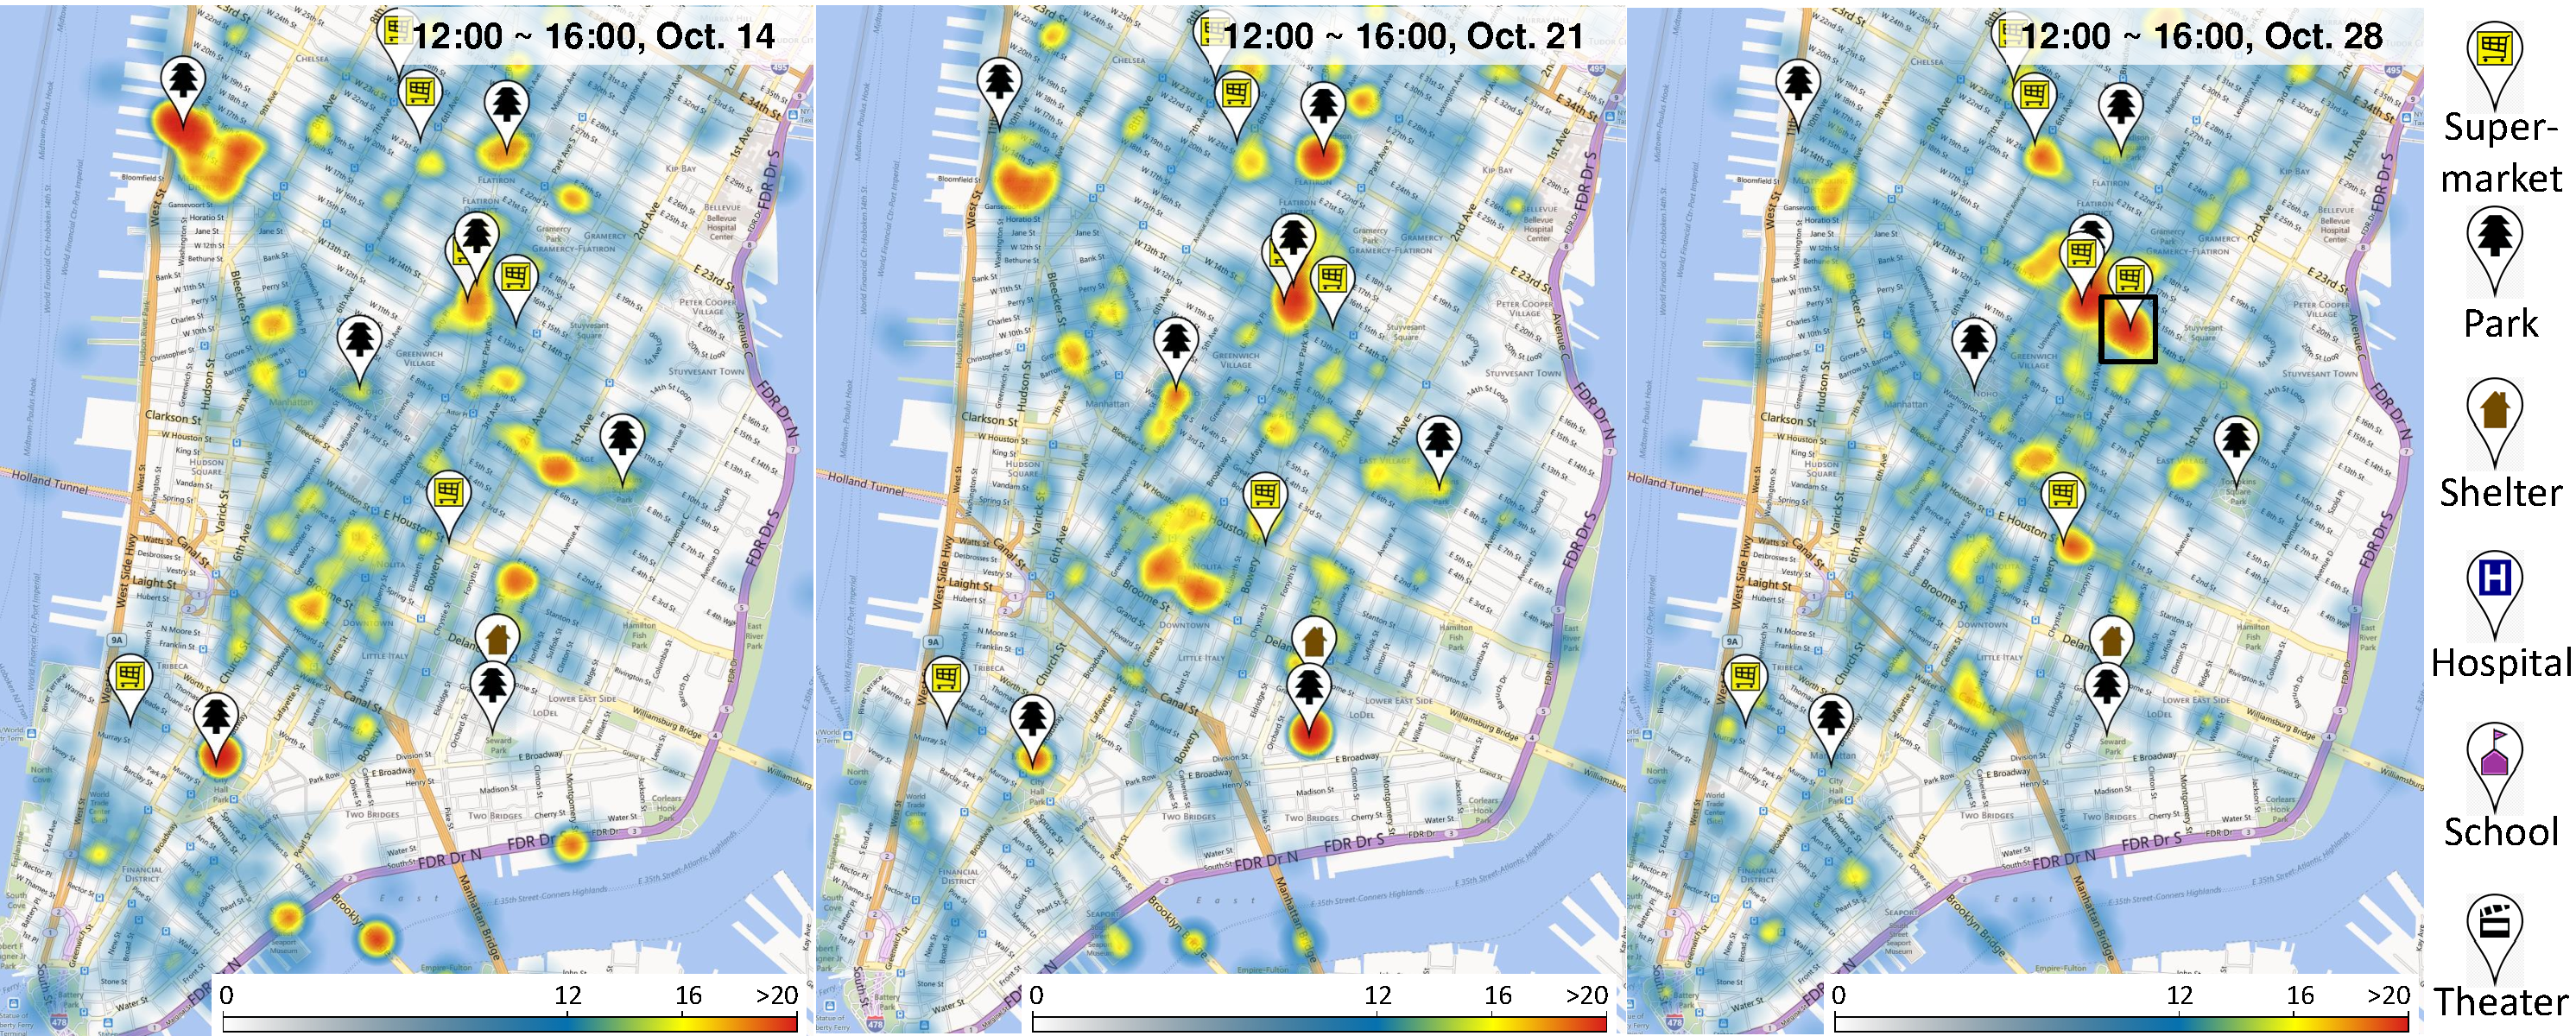
\includegraphics[width=0.9\linewidth]{heatmap_manhattan_v3}
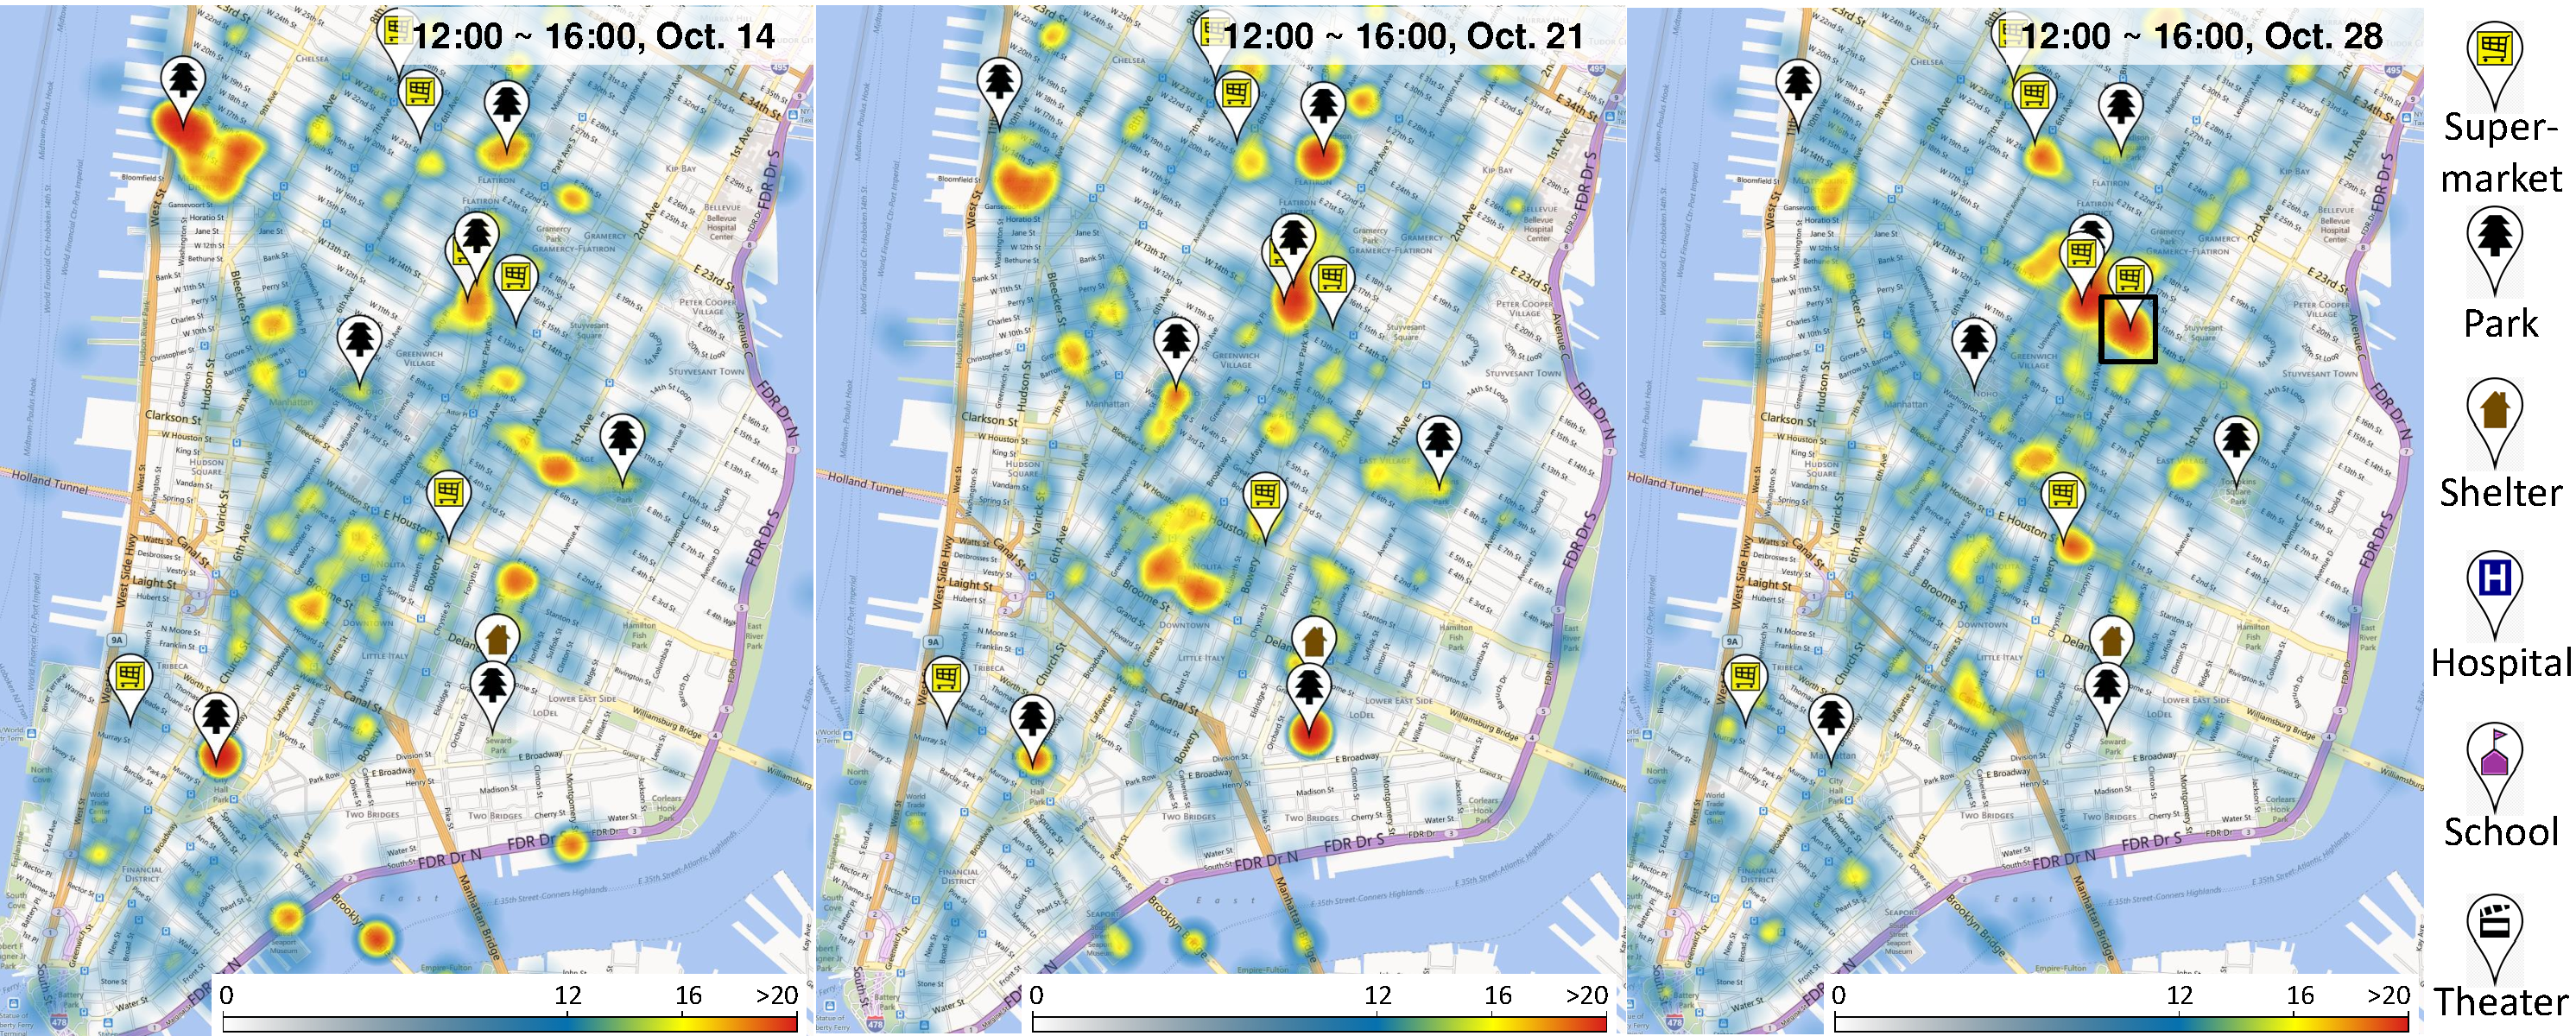
\includegraphics[width=1.0\linewidth]{heatmap_manhattan_v3}
\caption{Spatial user-based Tweet distribution in the Manhattan area in New York City during four hours right after the evacuation order (from 12:00 PM to 4:00 PM on October 28th, 2012 (Right)). Previous distribution of Tweets on 14th (Left) and 21st (Center).}
\label{fig:heatmap_manhattan}
%\vspace{-0.4cm}
\end{figure}

In late October in 2012, a massive hurricane, Sandy, devastated Northeastern United States~\cite{WKP:2012:SANDY}.
Due to the severeness of the hurricane,  on October 28th in 2012, the New York City Authorities ordered residents to leave some low-lying areas\textemdash the mandatory evacuation zones (red color) are shown in Figure~\ref{fig:spatiotemporal} (Right).
%Shelters were opened in the morning on October 28th ahead of the storm approaching the eastern third of the United States \-- the mandatory evacuation zones (red color) are shown in Figure~\ref{fig:spatiotemporal} (Right).
We investigate an area of Manhattan, since the area is the most populated and severely damaged.
Through the map view in our system, analysts navigate to the Manhattan area in New York City and filter Tweets posted within the area. 
%appearing in the view during two weeks before and after October 28th.
Initially we tried to reveal public movement flows during the disaster event, but the movement patterns were too complicated to find meaningful flows due to movement randomness and the visual clutter of the flows.
Then, we examined the spatial distribution of the users for specific time frames.
Based on our experiments, a geospatial heatmap was useful for an overview of the spatial distribution and for trend approximation.
We utilize a divergent color scheme to generate the heatmap, where saturated colors are used for the data distribution to avoid any confusion from the color scheme from the desaturated colormap of the background map.
Analysts can specify a threshold range to emphasize hotspots, where the upper bound is mapped to a red color and the lower bound to a yellow color.
Additionally, the blue color is mapped by the analysts to the value of the overall distribution of Twitter users.
In Figure~\ref{fig:heatmap_manhattan}, we show three heatmaps of spatial user-based Tweet distribution from 12:00 PM to 4:00 PM on October 14th (Left), 21st (Center), and 28th (Right).
In this work, we use the number of Twitter users instead of the number of Tweets for the heatmap generations to properly reflect the flow of evacuation unbiased by personal Tweet activity or behavior of individual users, since some enthusiastic Twitter users generate a large number of Tweets at the same location during a short time period (more than 20 Tweets per hour).
The heatmaps in Figure~\ref{fig:heatmap_manhattan} (Left and Center) represent normal situations of Twitter user distribution in the Manhattan area, and the heatmap (Right) shows the situation right after the evacuation order that was announced at 10:30 AM on October 28th, 2012.
This standard heatmap visualization allows analysts to explore the spatial pattern of Twitter users for any specified time period.
In Section~\ref{sec:spatial_decision_support}, we will provide further analysis for the spatial decision support.

\begin{figure}[tbh]
\centering
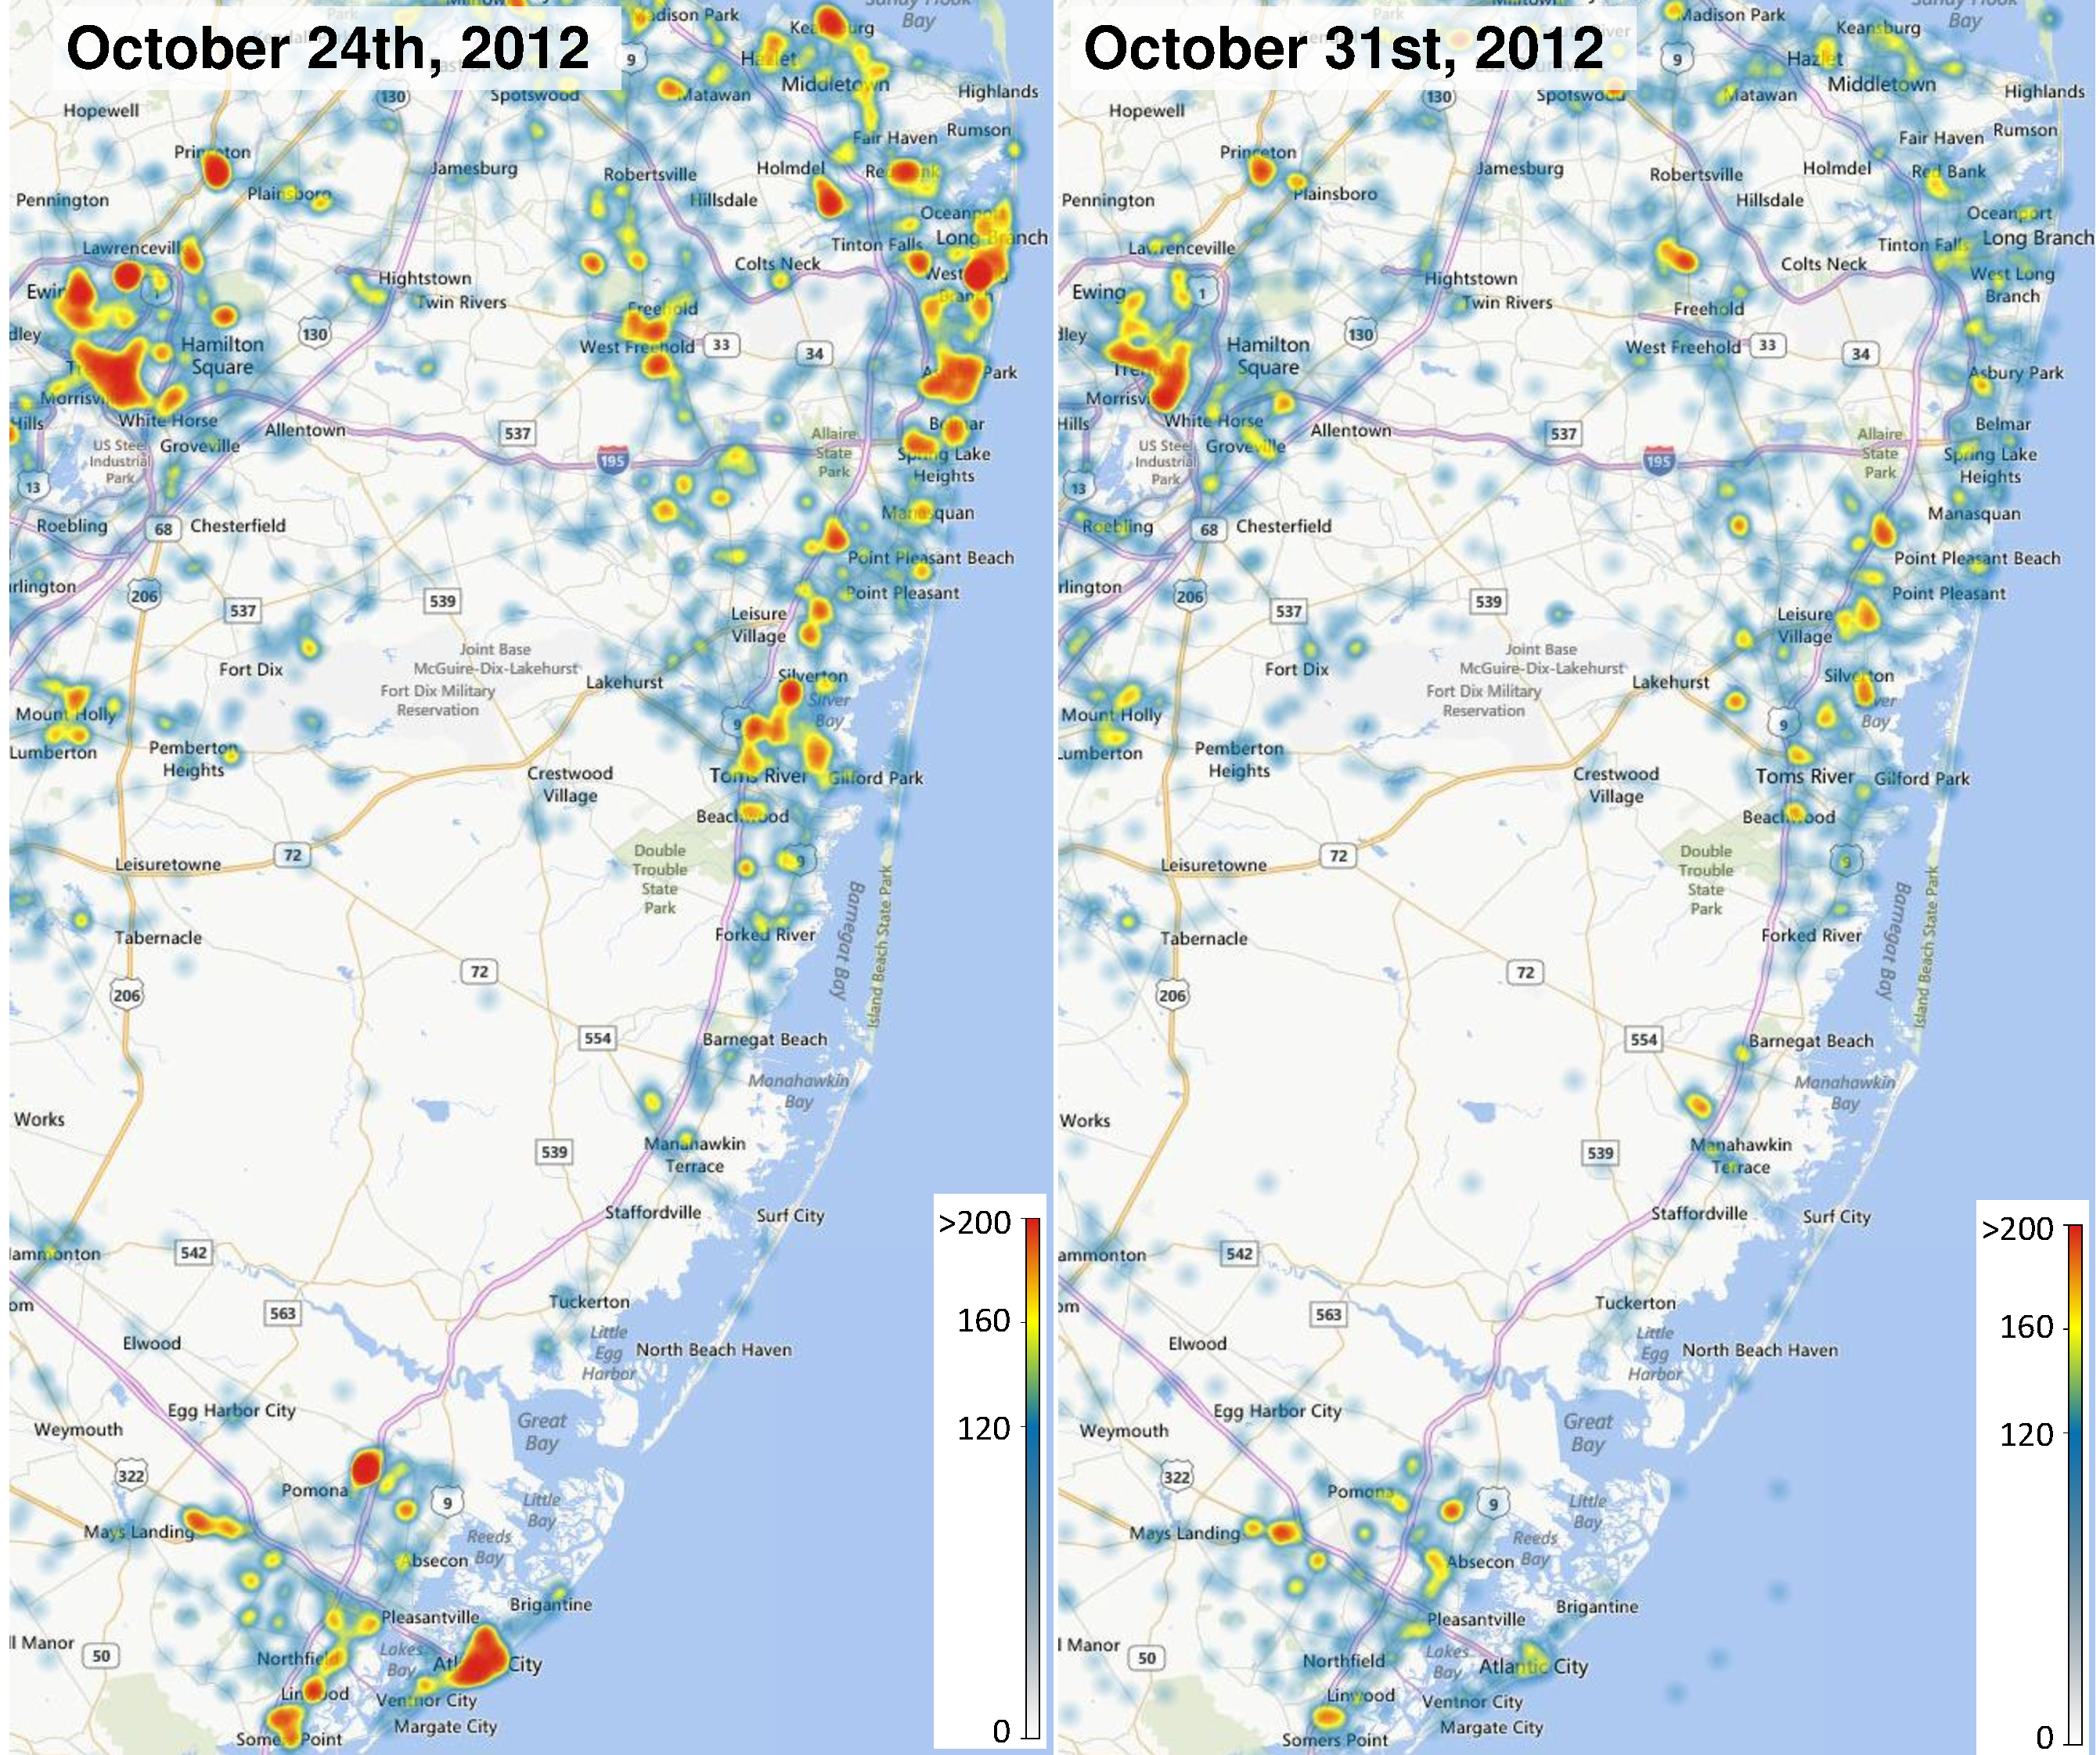
\includegraphics[width=1.0\linewidth]{Atlantic_Coast_v6}
\caption{Twitter user distribution on the eastern coast area in New Jersey, after the hurricane passed over the area on October 31st (Right). Previous distribution on October 24th is shown on the Left.}
\label{fig:atlantic_coast}
%\vspace{-0.4cm}
\end{figure}

Hurricane Sandy damaged not only New York City, but also the entire eastern coast area of New Jersey. 
Most cities in the area also announced evacuation orders on October 28th, 2012.
The distribution of Twitter users in the area from Atlantic City to the upper eastern shore area for two different dates are shown in Figure~\ref{fig:atlantic_coast}.
The heatmaps in Figure~\ref{fig:atlantic_coast} (Left) represent the previous normal situation of Twitter user distribution on October 24th and the heatmap (Right) shows the post distribution after Sandy passed over the area on October 31st.
As shown in the result, many hotspots are gone or diminished.
This situation shows that the number of Twitter users had significantly decreased after the hurricane damaged the area.
In fact, a huge number of homes were damaged or destroyed and a couple of million households lost power because of Hurricane Sandy~\cite{WKP:2012:EHS}.
In disaster management this type of visualization can support analysts estimating which areas were highly damaged and even which areas still need reconstruction.



%
%\begin{figure}[tb]
%\centering
%\includegraphics[width=0.8\columnwidth]{symbols}
%\caption{Standard symbols for infrastructures used in the paper~\cite{Robinson:2012:DMS}.}
%\label{fig:symbols}
%\vspace{-0.5cm}
%\end{figure}
%
%
%




\subsection{Spatial Decision Support}
\label{sec:spatial_decision_support}
%Investigating and making decisions using only the heatmap without any supplementary information are demanding and hard to unserstand the actual events.
In Section~\ref{sec:spatial_analysis}, we introduced our spatial analysis to explore the Twitter user distribution.
In addition to the analysis, our system allows the analysts to utilize supplementary information in order to support understanding of the situations and decision-making in disaster management.
The spatial characteristics together with heterogeneous information can assist in disaster management and migrating hazards where the problems have spatial components~\cite{Andrienko:2007:GAS}.
The supplementary information can be various types of infrastructures (i.e., school, park, supermarket, and shelter), as well as spatial information of disaster events (i.e., hurricane path and damage area of a tornado).
In this section, we describe how our system supports spatial decision-making by correlating such spatial information with location-based microblog data.

\subsubsection{Infrastructure Data}
\label{sec:infrastructure_data}
%
During a natural disaster event, such as Hurricane Sandy, analysts would assume that many people might want to go to the supermarket before staying or evacuating, but they would need supporting evidence before making appropriate decisions and plans.
With our system support, the analysts can simply overlay the locations of large supermarkets on the heatmap of the Twitter user distribution.
The infrastructure locations are indicated by standard symbols~\cite{Robinson:2012:DMS} as 
shown on the right side of Figure~\ref{fig:heatmap_manhattan}.
%presented in Figure~\ref{fig:symbols}.
%(e.g., \textit{Trader Joe's} and \textit{Whole Foods Market}).
%Note that there is no major retail chains, such as Walmart and Target in Manhattan.
A relatively large number of people immediately went to supermarkets nearby the evacuation area, instead of the emergency shelter as shown in Figure~\ref{fig:heatmap_manhattan} (Right).
However, October 28th was Sunday and many people generally would go for grocery shopping on Saturday or Sunday; therefore, the analysts might need to verify whether the heatmap shown in the figure is a normal periodic situation.
The analysts can investigate new Twitter user distributions for different time frames by simply manipulating the time context.
In Figure~\ref{fig:heatmap_manhattan} (Left and Center), we show two distributions for one and two weeks before the disaster period respectively.
Here, we see that the hotspot locations are very different from the ones for October 28th shown in Figure~\ref{fig:heatmap_manhattan} (Right).
For further analysis, we can explore another popular Sunday location\textemdash large parks\textemdash by superimposing the locations on each heatmap.
%, since we can expect that parks would be populated on Sunday.
As shown in Figure~\ref{fig:heatmap_manhattan} (Left and Center), many hotspots overlap with the park areas in normal situations.
Therefore, we can conclude that the situation on October 28th is an unusual non-periodic pattern.
%
%This system can support the analysts to understand the unusual movement patterns and plan resource allocation accordingly for such emergency events.
%
%can realize that the situation on October 28th is unusual and non-periodic. 
%This system can support them to make plans for preparing some responses for the emergency events.



\subsubsection{Disaster Event Data}
\label{sec:event_data}
%
In Section~\ref{sec:infrastructure_data}, we explained how the infrastructure data help the analysts to understand and examine the emergent situations.
During severe weather conditions, people tend to be sensitive to the dynamic variance of the weather conditions.
Relationship analysis, therefore, between the public responses and the spatiotemporal pattern of the severe weather is important.
Our system overlays geographic information of disaster events, for example, center positions and tracks of a hurricane, and damaged areas by a tornado, in order to provide further analysis.
Two case studies are presented as follows:

\textbf{Track of Hurricane:} Figure~\ref{fig:east_coast}~(1) and (2) show the southeastern coast areas of the United States, whereas,
Figure~\ref{fig:east_coast}~(3), (4), and (5) show the northeastern coast areas.
In the figures the distributions of Twitter users for each consecutive date, from October 26th to 30th, 2012, are presented 
using the heatmap visualizations.
We use the number of Twitter users who posted Twitter messages containing one of the following keywords: \textit{hurricane, storm}, and \textit{sandy} in order to analyze Tweets that are highly related to Hurricane Sandy.
Note that Hurricane Sandy reached the southeastern Florida coast on October 26th and passed, then, over the northeastern coast on October 30th, 2012~\cite{WKP:2012:SANDY}.
As shown in Figure~\ref{fig:east_coast}, our system is able to overlay the track of the hurricane on the map.
% according to a time period of interest.
%(the texts on the map were manually added).
The blue pins and the blue lines represent the center locations of the hurricane and its path respectively.

\begin{figure}[tbh]
\centering
%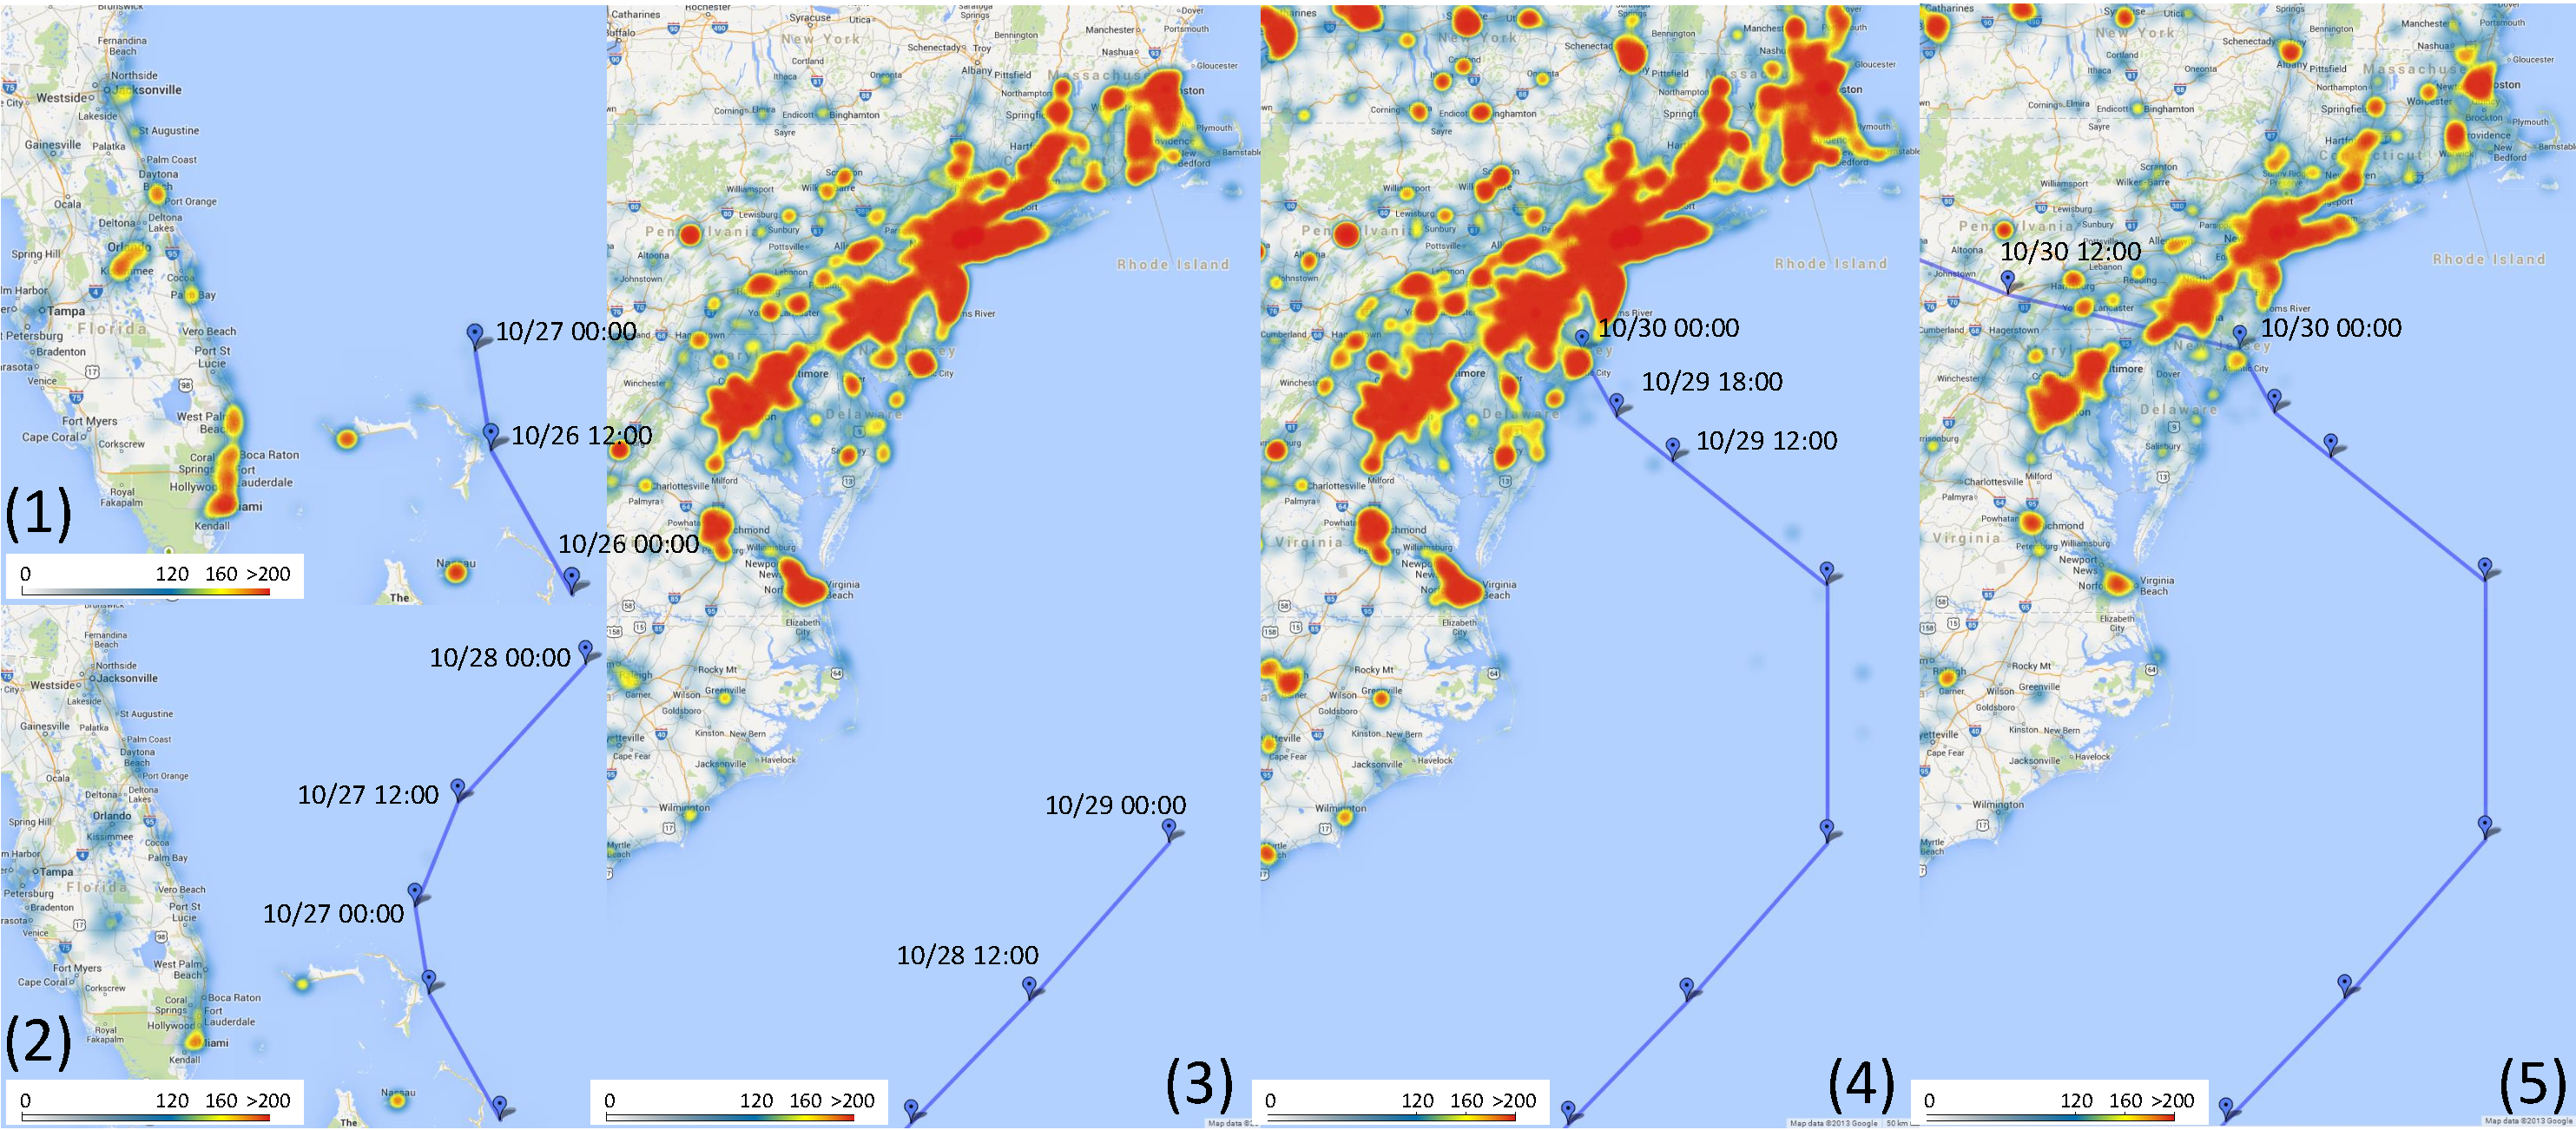
\includegraphics[width=0.85\linewidth]{East_Coast_v7}
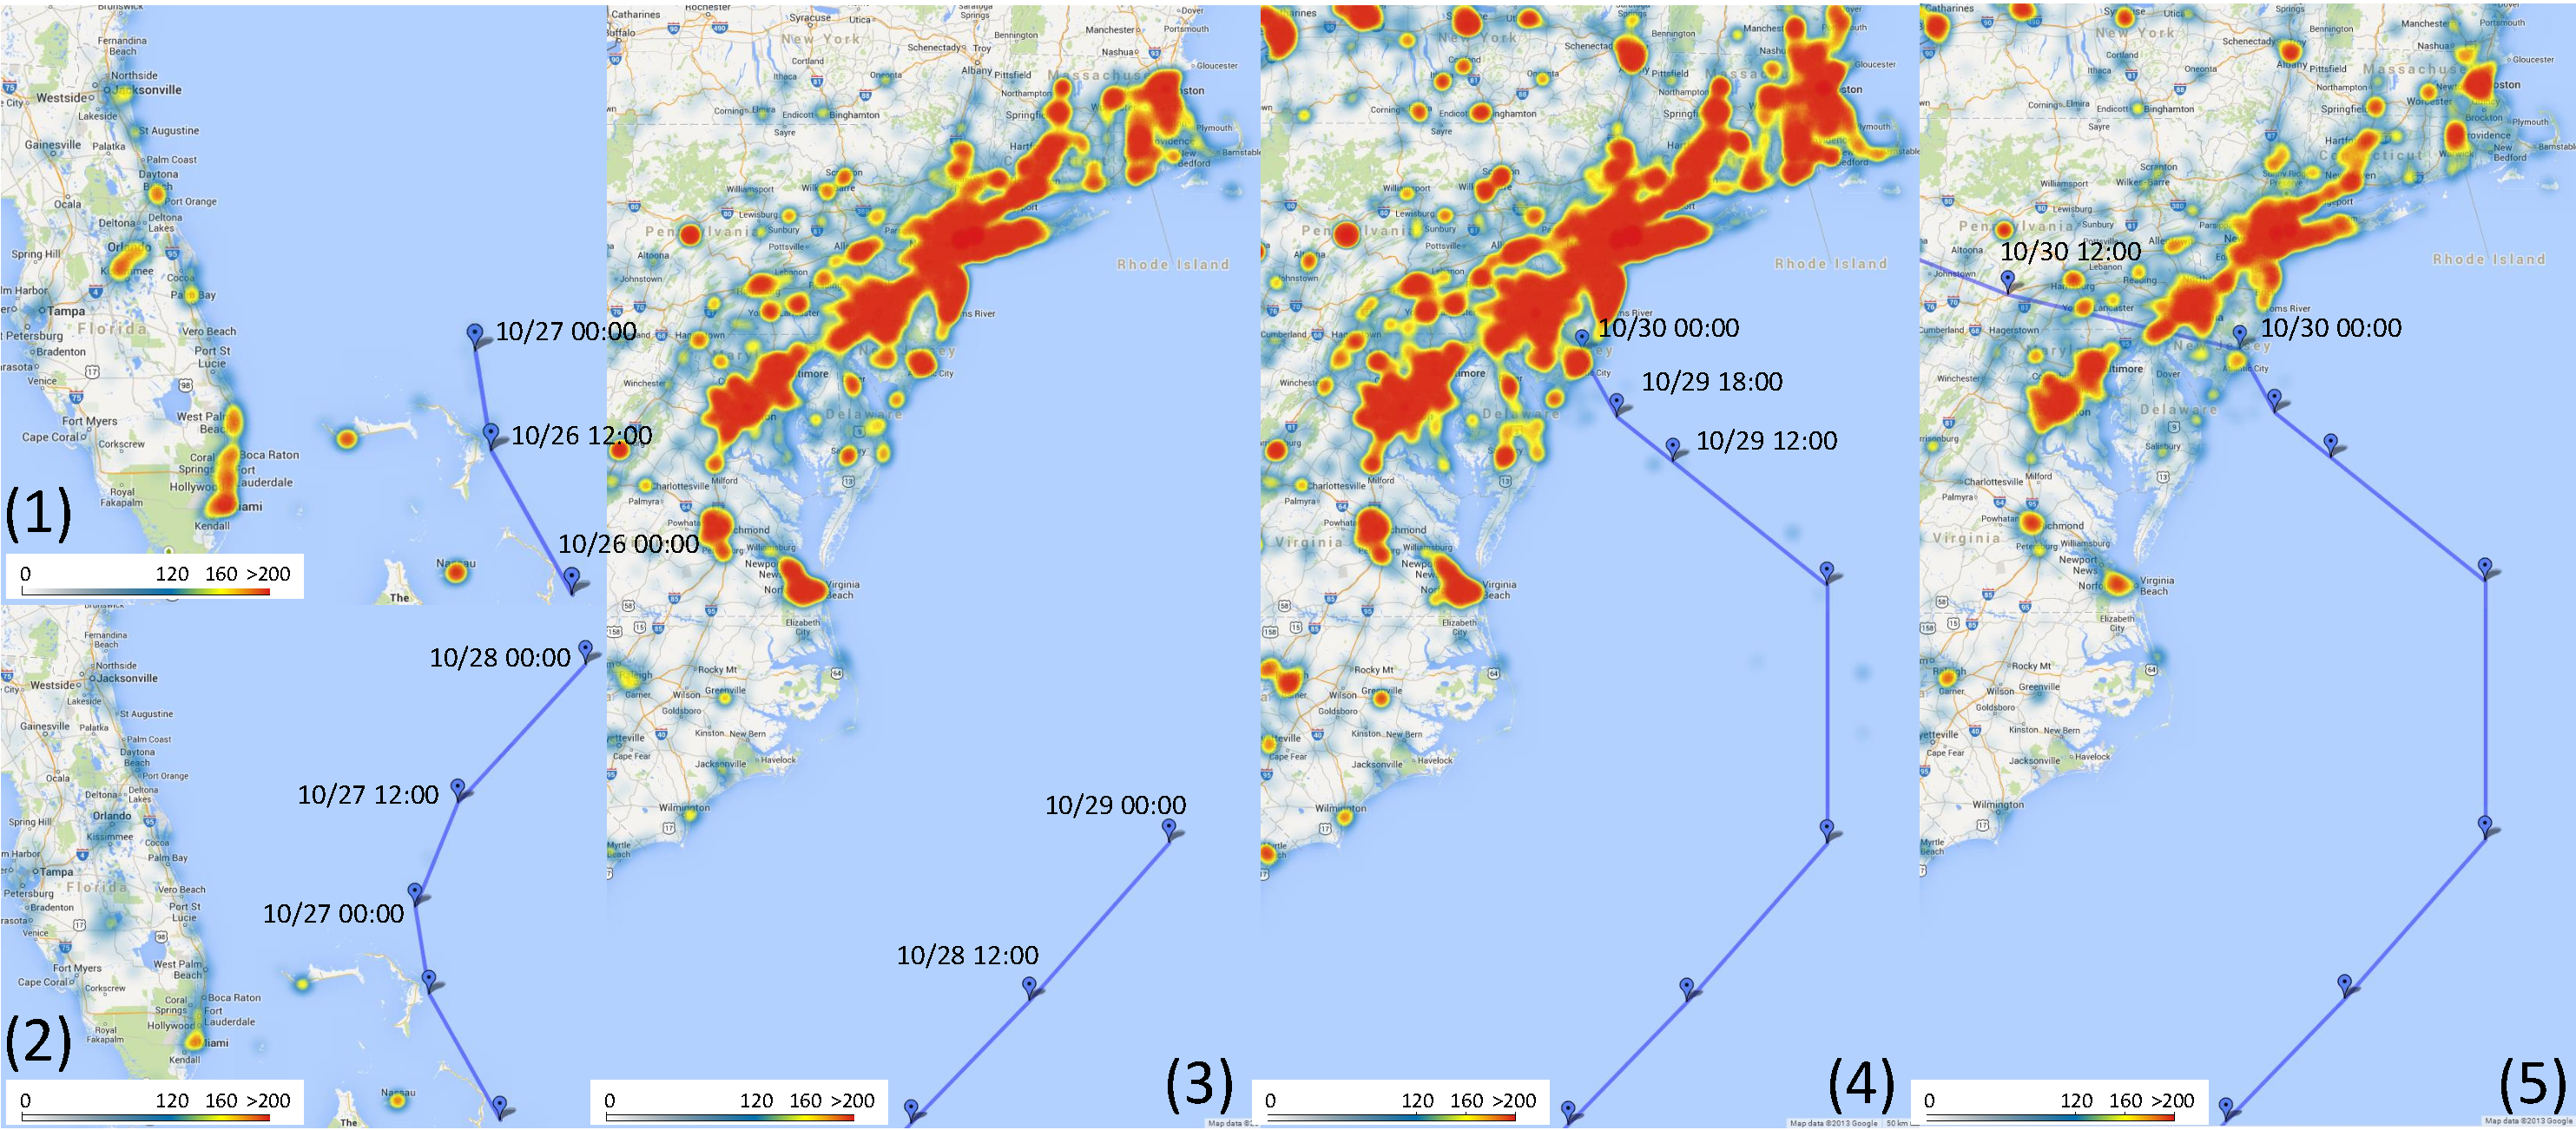
\includegraphics[width=1.0\linewidth]{East_Coast_v7}
\caption{Distribution of Twitter users of each consecutive date (Oct. 26 $\sim$ 30, 2012), who post hurricane related Tweets on the southeastern (1 and 2) and northeastern coast (3, 4, and 5) area of the United States. We can see the variance of Twitter user reactions along the track of the hurricane center locations.}
\label{fig:east_coast}
%\vspace{-0.4cm}
\end{figure}

Twitter users also actively respond to the severe weather conditions.
In Figure~\ref{fig:east_coast}, we indicate that the distribution pattern of Twitter users had dynamically varied along the track of the hurricane center locations.
When Sandy moved to the southeastern coast on October 26th, there were bursts on eastern Florida's coast (Figure~\ref{fig:east_coast}~(1)).
Next day, the bursts disappeared, because Sandy moved towards the northeast away from the east coast of United States (Figure~\ref{fig:east_coast}~(2)).
Sandy kept moving towards a few hundred miles southeast of North Carolina on October 28th (Figure~\ref{fig:east_coast}~(3)).
In the next day, the hurricane's track bent towards the north and the hurricane made landfall at night in the northeast of Atlantic City 
(Figure~\ref{fig:east_coast}~(4)).
Throughout the days, Twitter users were actively reacting to Hurricane Sandy' arrival in a wide range of areas.
After the landfall, the storm turned toward the northwest and was gradually weakened.
The big outbreaks were diminished on October 30th as shown in Figure~\ref{fig:east_coast}~(5).
As shown in the figures, we can see how Twitter users reacted according to the spatiotemporal pattern of the severe weather conditions in the social media domain.
%The Twitter user distributions along the track of the hurricane helps the users to understand the situations and further analysis.

%\textbf{Damage Area along the Tornado's Path:} 
\textbf{Damage Area from a Tornado:} An extremely strong Tornado passed through the city of Moore in southern metropolitan Oklahoma City~\cite{WKP:2013:MOORE} in the afternoon on May 20th, 2013.
The larger than one-mile-wide tornado damaged the city with a wind speed of more than 200~mph.
Figure~\ref{fig:tornado} shows the damaged part of the city.
The tornado entered the area at about 3:16 PM and exited the area after about 10 minutes.
We visualize the distribution of Twitter users on the map during 24 hours, from May 20th 4:00 PM to 21st 4:00 PM.
%This result represents the situation after the city was severely damaged by the tornado.
We also overlay an approximate extent of tornado damage (transparent orange color) and locations of multiple infrastructures, such as schools, hospitals, and supermarkets, on the map view.
Since the tornado suddenly happened and disappeared, we were not able to find significantly abnormal patterns before and during the event. 
%In Section~\ref{sec:discussion}, we will discuss about this in detail.
After the disaster event, however, many Twitter users moved toward some specific areas: two elementary schools, a medical center, a theater, and two large supermarkets.
The two elementary schools, the medical center, and the theater were located within the highly damaged area and they were severely destroyed.
Also many people were hurt and died in these infrastructures.
The increased number of Twitter users was probably due to the fact that many people went to these places in order to rescue the victims~\cite{TWITCHY:2013:CHG}.
Moreover, people might have gone to supermarkets to obtain indispensable things.
In Figure~\ref{fig:tornado}~(1), the heatmap shows a normal situation of Twitter user distribution in the same area.
The distribution is very different from the situation after the tornado hit the area.
This example demonstrates how our visual analytics system enables the analysts to analyze public responses using spatial disaster data and infrastructure data for disaster management.

\begin{figure}[tbh]
\centering
%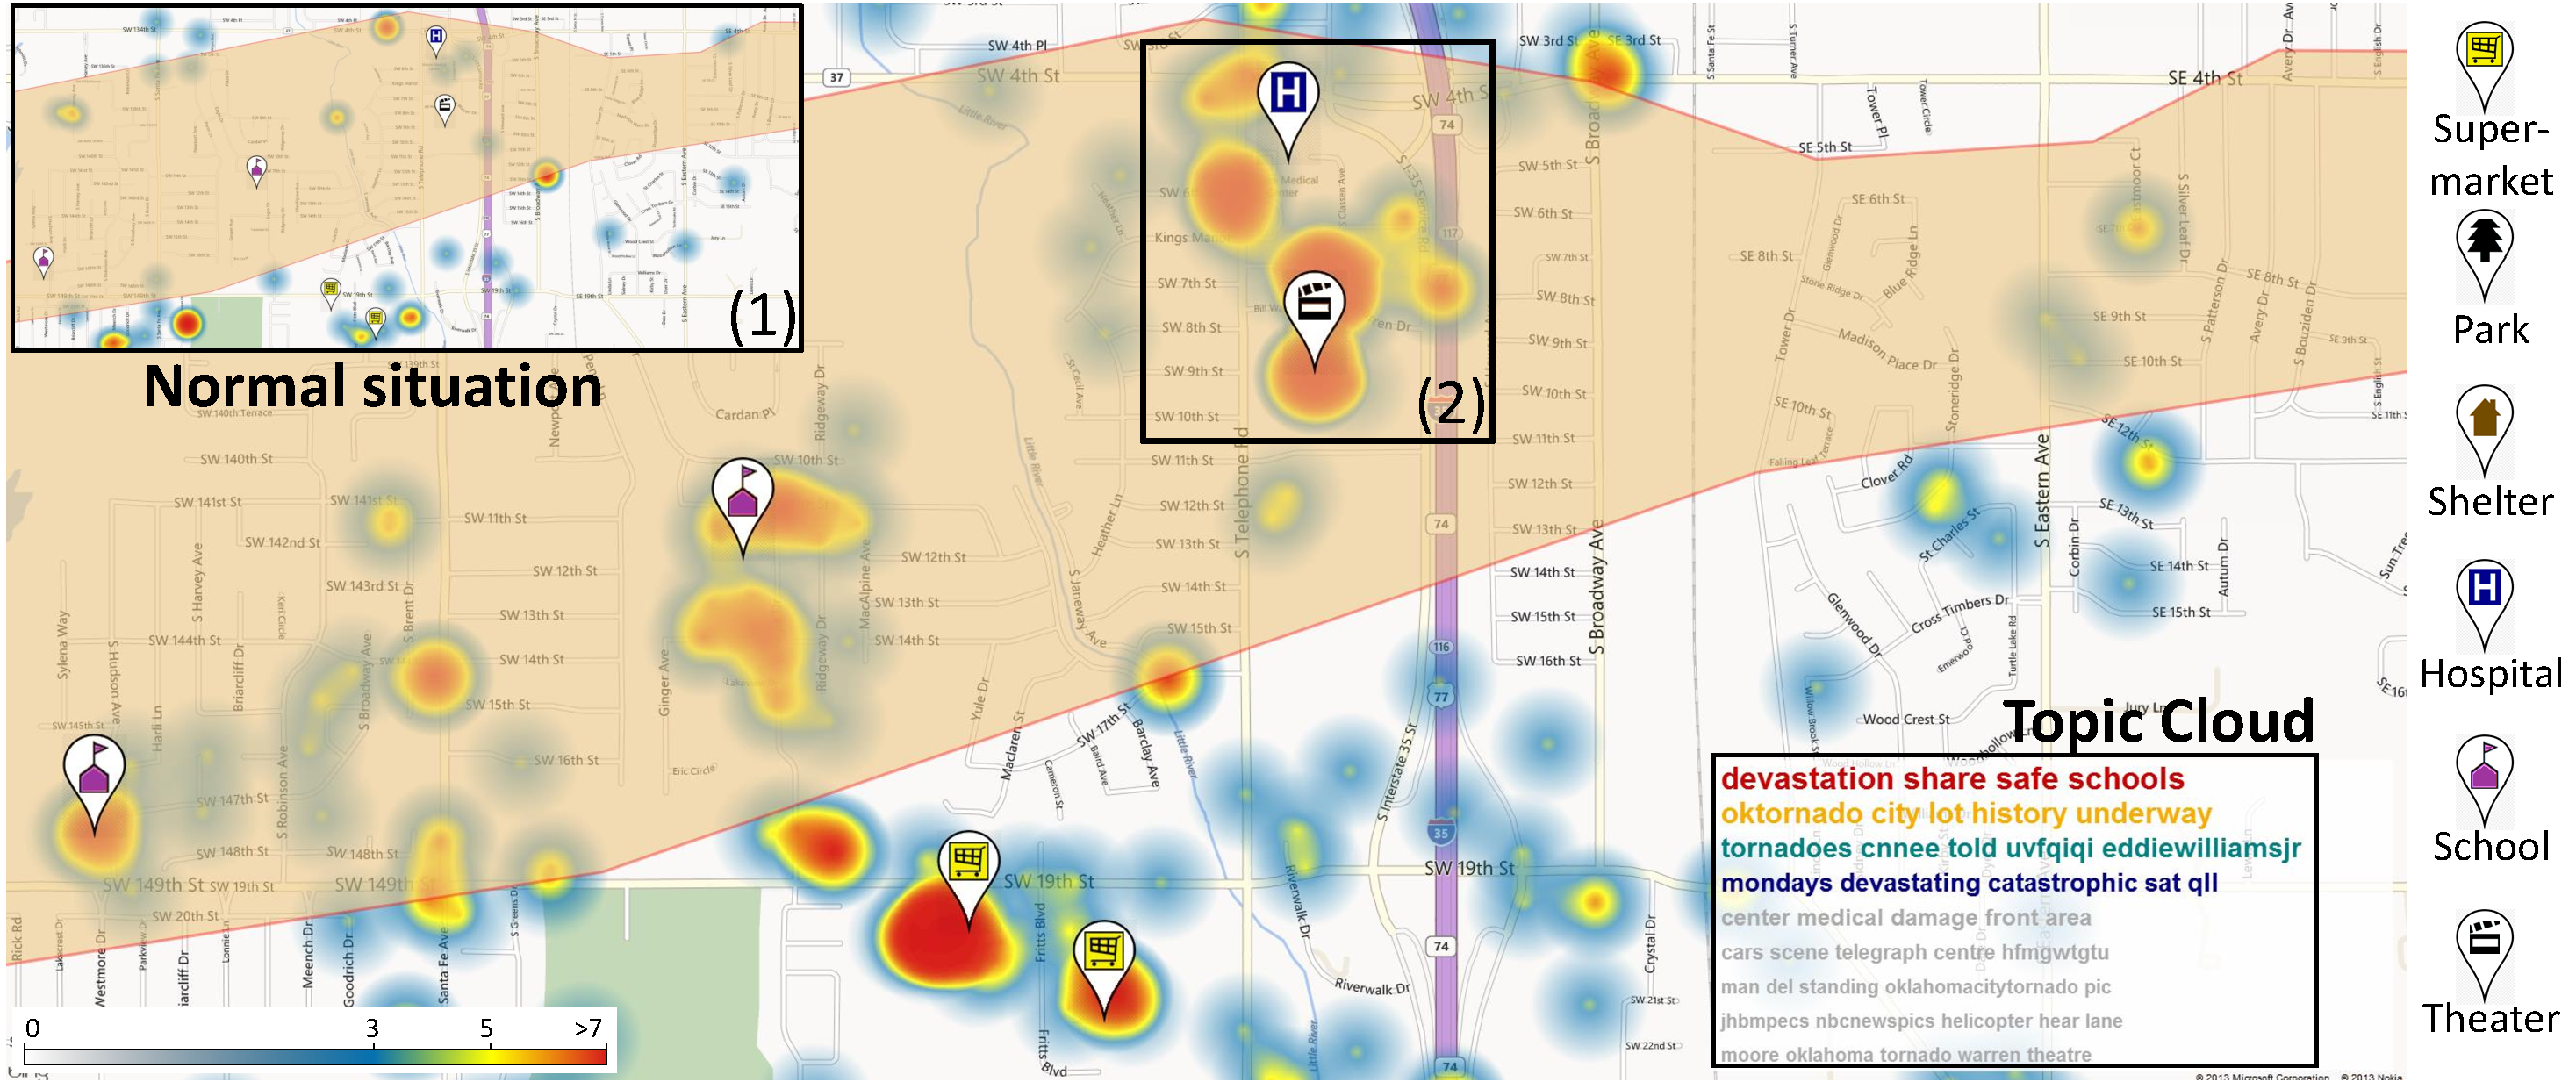
\includegraphics[width=0.9\linewidth]{Tornado_v9}
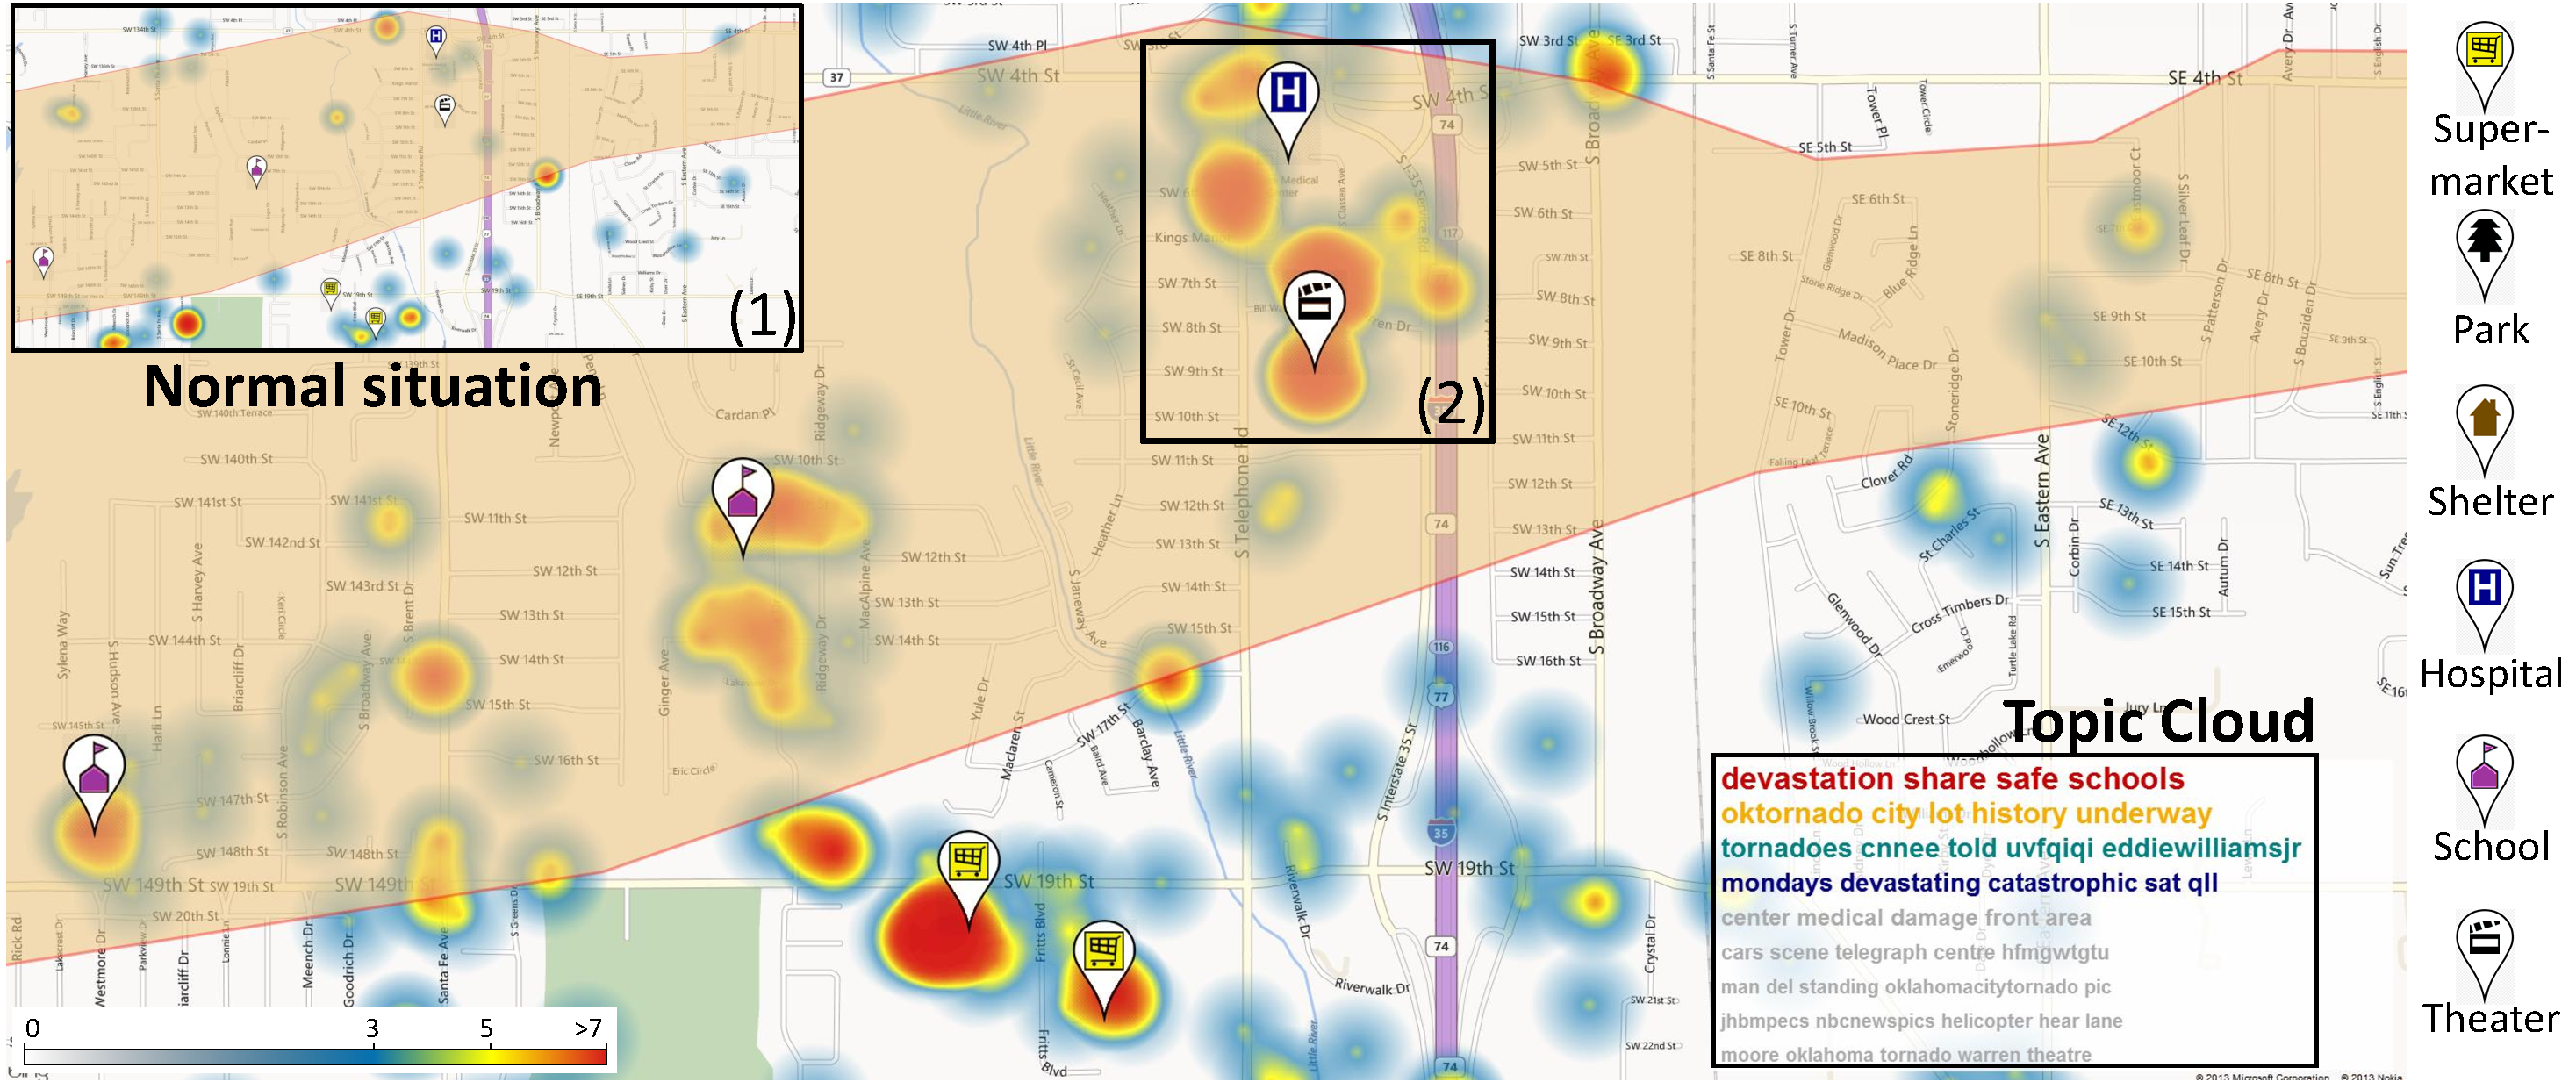
\includegraphics[width=1.0\linewidth]{Tornado_v9}
\caption{Spatial pattern of Twitter users during 24 hours in the city of Moore after damages from a strong tornado. Relatively many people moved to severely damaged areas after the disaster. This situation is much different from the previous normal situation (1). We selected a specific region (2) that includes severely damaged areas in order to extract topics (3) from Tweets within the selected area.}
\label{fig:tornado}
%\vspace{-0.2cm}
\end{figure}

\subsubsection{Abnormal Topic Analysis}
\label{sec:abnormal_topic_analysis}
\begin{figure}[tb]
\centering
%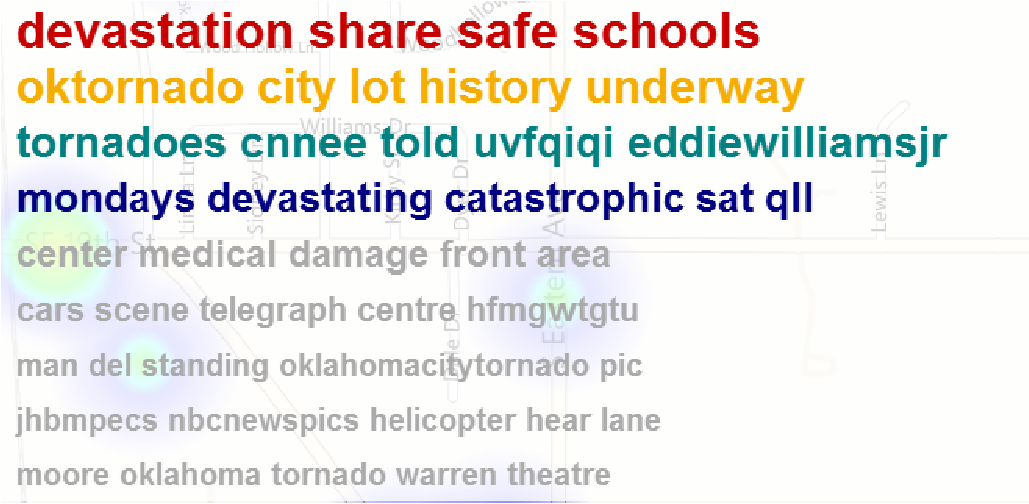
\includegraphics[width=0.85\columnwidth]{Topiccloud_v2}
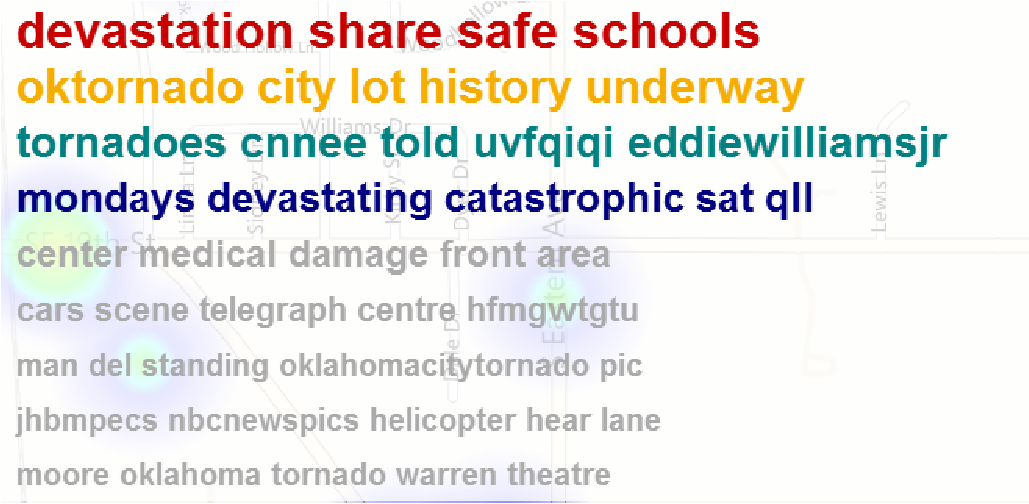
\includegraphics[width=0.8\linewidth]{Topiccloud_v2}
\caption{Topic cloud: Topics from Tweets within the selected area in Figure~\ref{fig:tornado}~(2) are ordered by their abnormality scores.}
\label{fig:topic_cloud}
%\vspace{-0.4cm}
\end{figure}

Our system also provides analysts with abnormal topic examination within the microblog data.
Each Twitter message provides not only spatiotemporal properties, but also textual contents.
The text messages are also important to understand and examine the emergent situations.
Our system allows the analysts to extract major topics from many Tweets posted within a specific area using the LDA~\cite{Blei:2003:LDA}.
We also employ, then, the STL~\cite{Cleveland:1990:SAS} to identify unusual topics within the selected area.
For each extracted topic of the LDA topic modeling, our algorithm retrieves messages associated with the topic and then generates a time series consisting of daily message counts from their timestamps.
The time series can be considered as the sum of three components: a trend component, a seasonal component, and a remainder.
Under normal conditions, the remainder will be identically distributed Gaussian white noise, while a large value of the remainder indicates substantial variation in the time series.
Thus, we can utilize the remainder values to implement control chart methods detecting anomalous outliers within the topic time series.
We have chosen to utilize a seven day moving average of the remainder values to calculate the z-scores.
Note that we use the z-score as the abnormality score in this work.
If the z-score is higher than 2, events can be considered as abnormal within a 95\% confidence interval.
The details of these techniques are described in the previous work~\cite{CHAE:2012:SSM}.
We select a sub area in Figure~\ref{fig:tornado}~(2) that includes severely damaged areas: the selected region (black rectangle) on the map.
The extracted topics, which are ordered based on their abnormalities, are displayed as Topic Clouds at the bottom-right corner (Figure~\ref{fig:tornado}~(3)) on the map.
The topic cloud is enlarged and shown in Figure~\ref{fig:topic_cloud}.
In this case study, most topics are related to the disaster event. 
However, the last topic\textemdash \textit{moore, oklahoma, tornado, warren, theatre}, has a relatively low abnormality although they seem related to the disaster event, because tornadoes frequently occur in the area.
%Our abnormal topic analysis enables the analysts to understand what situations are going within the area.
Figure~\ref{fig:abnormality_graph} shows an abnormality graph for the first topic in Figure~\ref{fig:topic_cloud}.
The abnormality score for the topic had significantly increased when the tornado hit the region on May
20th (Marked region). As shown in Figure~\ref{fig:abnormality_graph}, the abnormality score (6.75) is much higher than the average abnormality score(0.42); therefore, the analysis of the microblog data provides a statistically significant difference during this severe weather condition.



\begin{figure}[tb]
\centering
%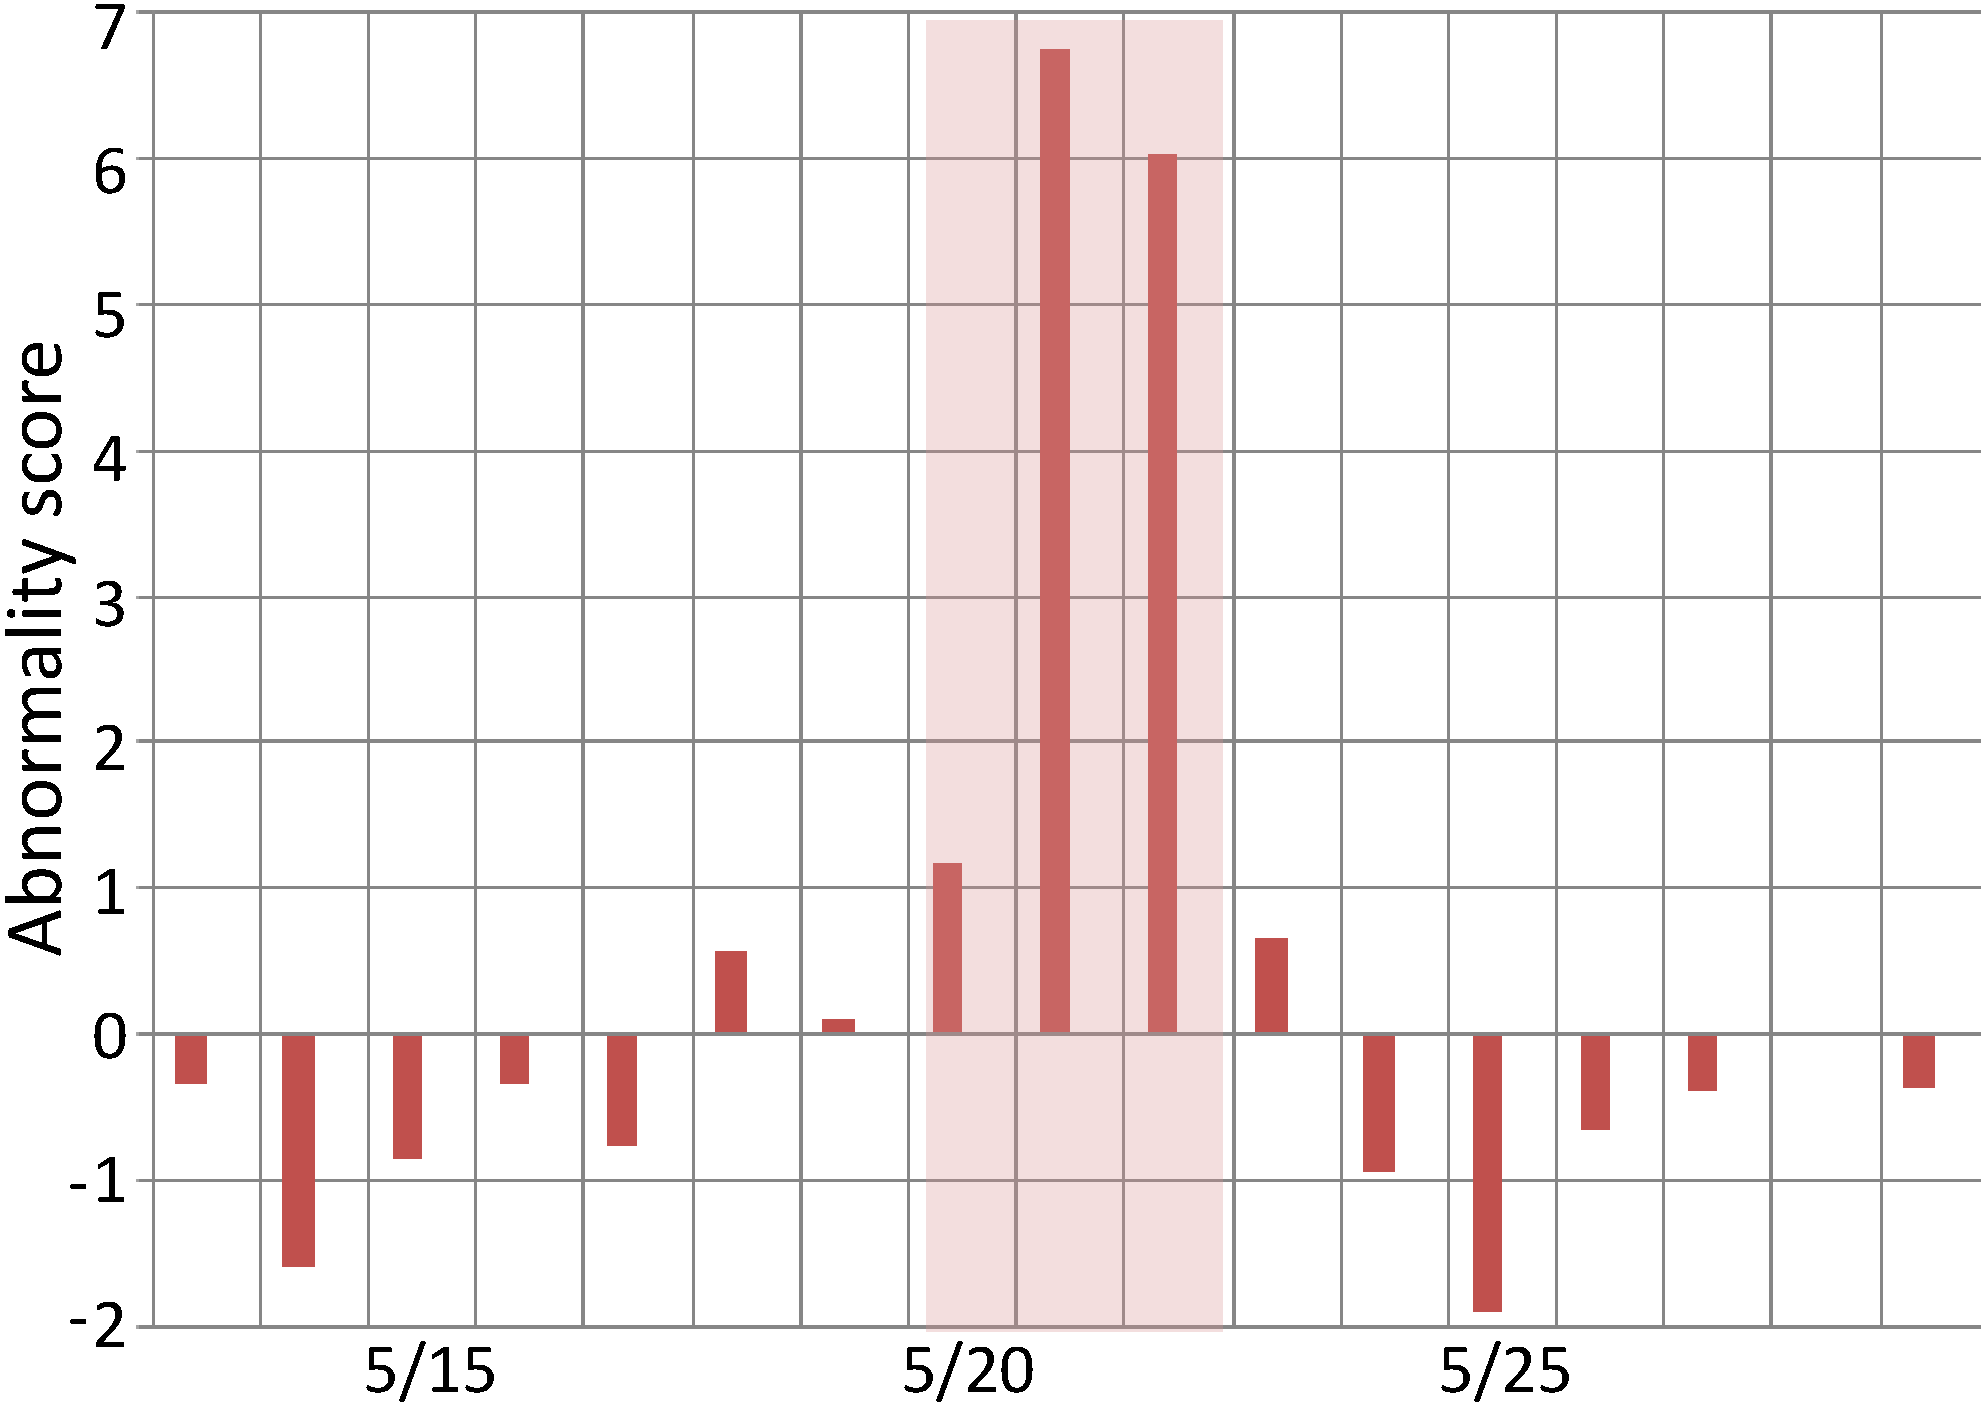
\includegraphics[width=0.7\columnwidth]{Topiccloud_zscore_graph_v3}
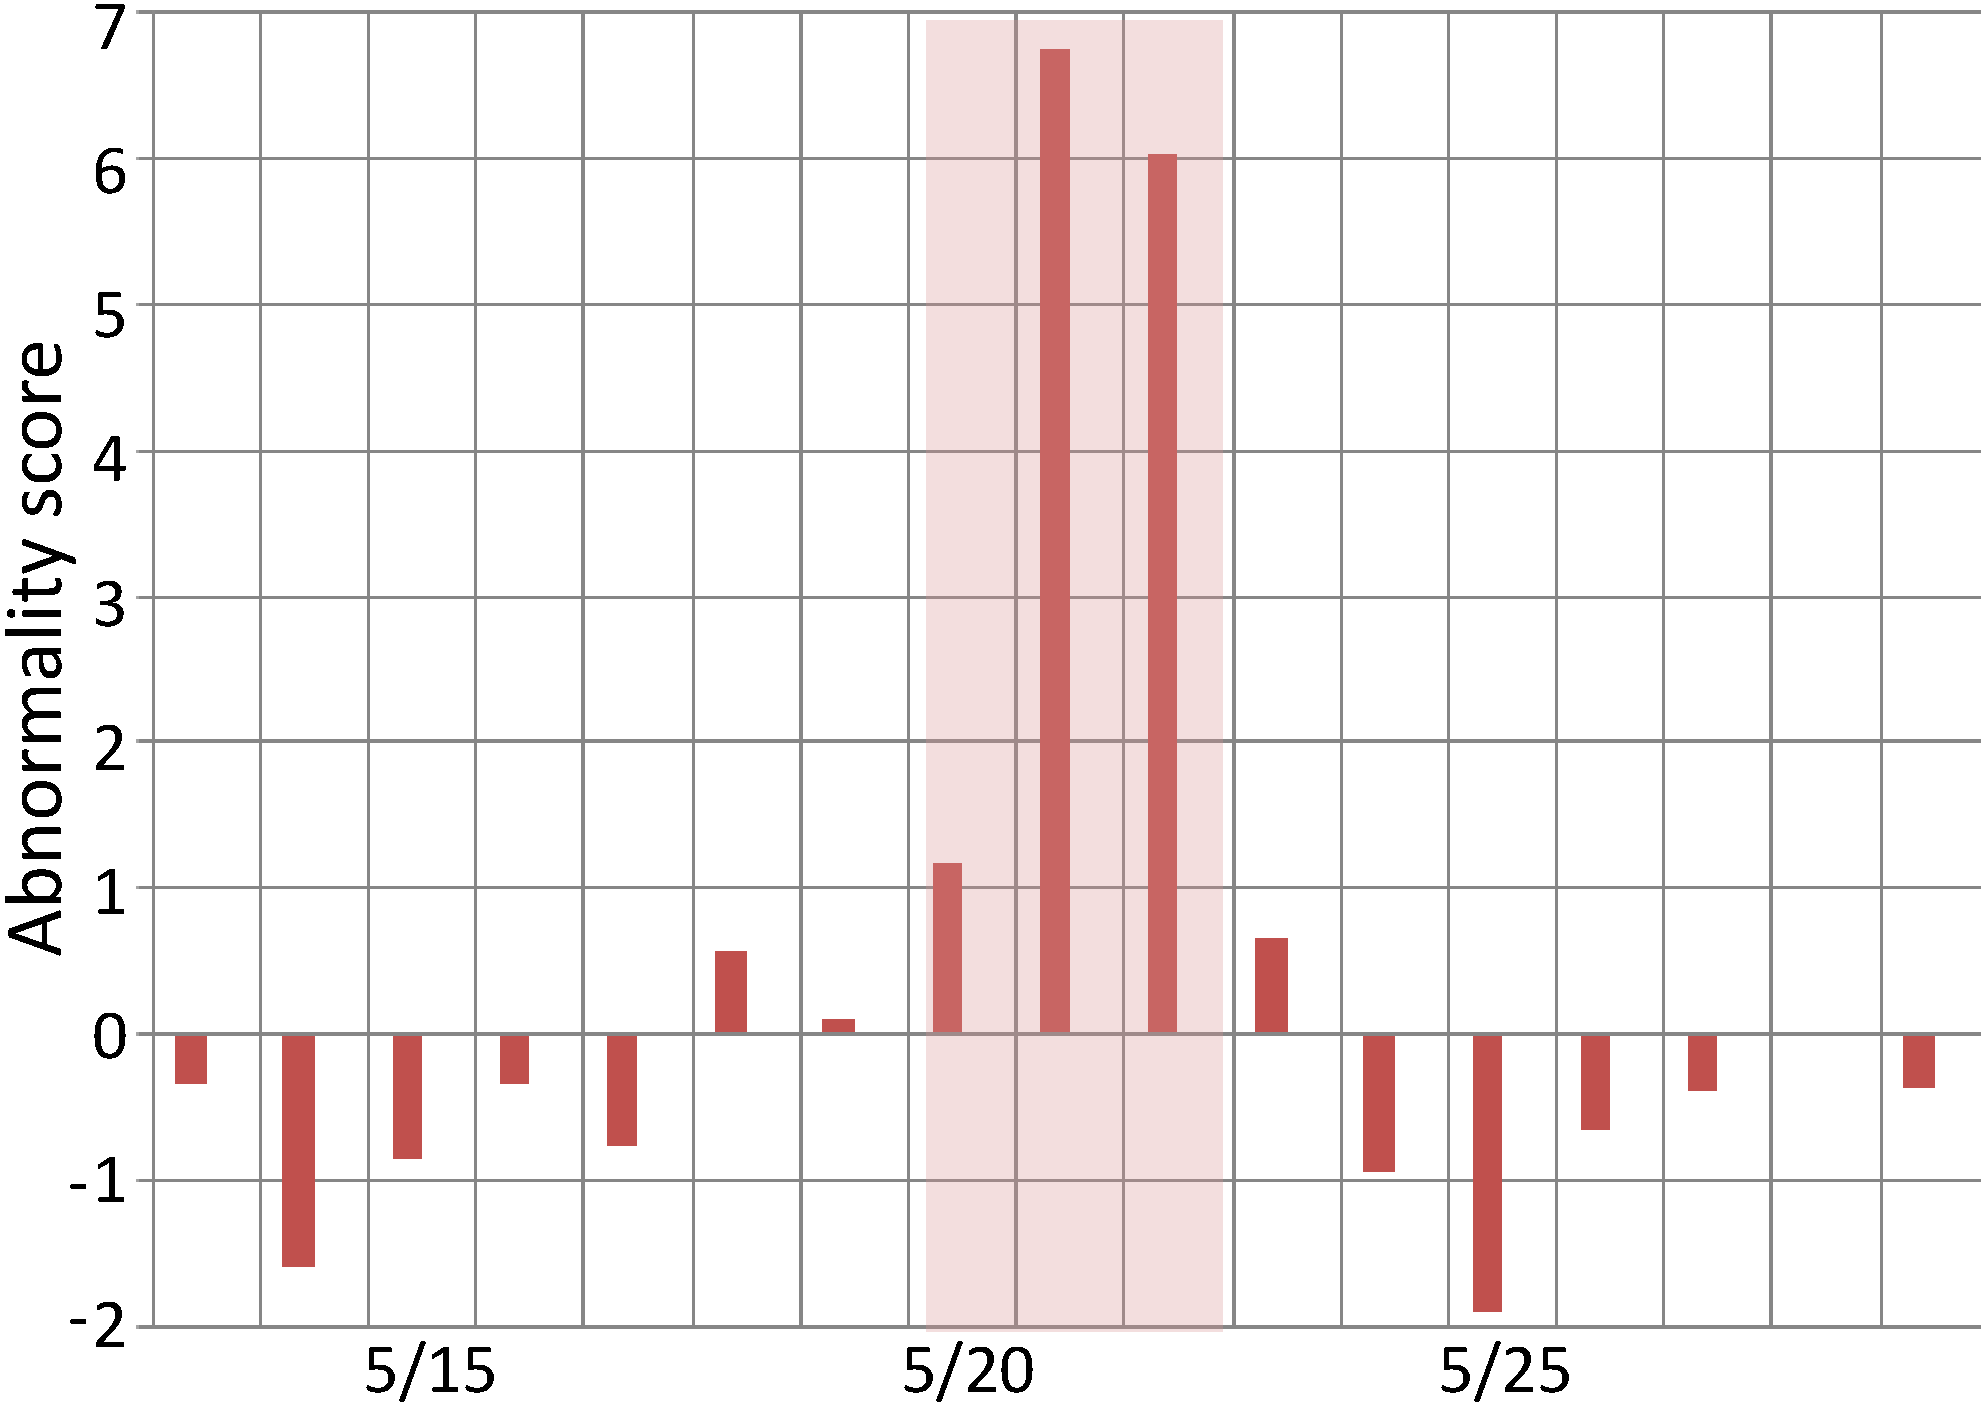
\includegraphics[width=0.8\linewidth]{Topiccloud_zscore_graph_v3}
\caption{Abnormality of the first topic in Figure~\ref{fig:topic_cloud}. 
The abnormality score of the topic had significantly increased when the tornado hit the region on May 20th (Marked region).}
\label{fig:abnormality_graph}
%\vspace{-0.4cm}
\end{figure}


\subsection{Temporal Pattern Analysis}
\label{sec:temporal_pattern}
%
%Describe the graph
%In Section~\ref{sec:spatial_analysis}, we present spatial analysis of social media and spatial decision support using multiple types of supplementary data in order to reveal where and why a number of people move.
In the previous sections, we presented the spatial analysis of social media and spatial decision support. 
In this section, we demonstrate analysis of the relationships between the temporal patterns of the number of Twitter users and certain public situational behaviors:
%using time-stamp information of Tweets
how many people go where and how different is it from previous situations?
Analysis of temporal trends and relationships between data values across space and time provides underlying insights and improves situational awareness~\cite{Maciejewski:2010:FHP, Malik:2011:DTC}.


After selecting the initial spatiotemporal context of Tweets as a basis for the analysis, the analysts can explore the temporal patterns of the number of Twitter users who posted Tweets within the spatial boundary using the bar chart as shown in Figure~\ref{fig:graph}.
The values of each bar are the number of users in four hour intervals and represent data two weeks before and after the selected date.
Once a mouse cursor hovers over one of the bars in the graph, every bar that corresponds to that time period, is highlighted in dark yellow color as shown in Figure~\ref{fig:graph}.
As previously mentioned, the heatmap in the figure shows the Twitter user density distribution from 12:00 PM to 4:00 PM on October 28th, right after the announcement of the evacuation order.
We select a hotspot that includes one of the supermarket locations: the selected region (black rectangle) on the map in Figure~\ref{fig:heatmap_manhattan} (Right).
We can indicate that the number of Twitter users (red rectangle in Figure~\ref{fig:graph}) in the corresponding time period is higher than for the same time period from other dates (October 14th, 21st and November 4th, 5th) by 35\% more from the average.
Moreover, there is another interesting finding\textemdash the number of people during each of the following time frame (4:00 $\sim$ 8:00 PM) on the dates from the previous weeks are higher than the number of people in the selected time frame.
This is because many shoppers were lining up at stores and emptied the shelves to prepare for Hurricane Sandy.
Some actual Twitter messages posted in the area are following: \textit{\textquoteleft The line at Trader Joes is unbelievable ...\textquoteright} and \textit{\textquoteleft There is amazing line here ...\textquoteright}.
Furthermore, since October 29th, the number of people has significantly decreased because most residents left the area before the arrival of the hurricane.
The increase in the number of people after one week reflects that some people came back to the area.
% and even shows when the stores reopened.

%Social media use rises during disasters as people seek immediate and in-depth information%~\cite{STAR}.
%reflect that the number users increased during sandy, but the situation had been gone since evacuation or severe damage for example, power outage caused by flooding and strong wind.

\begin{figure}[tbh]
\centering
%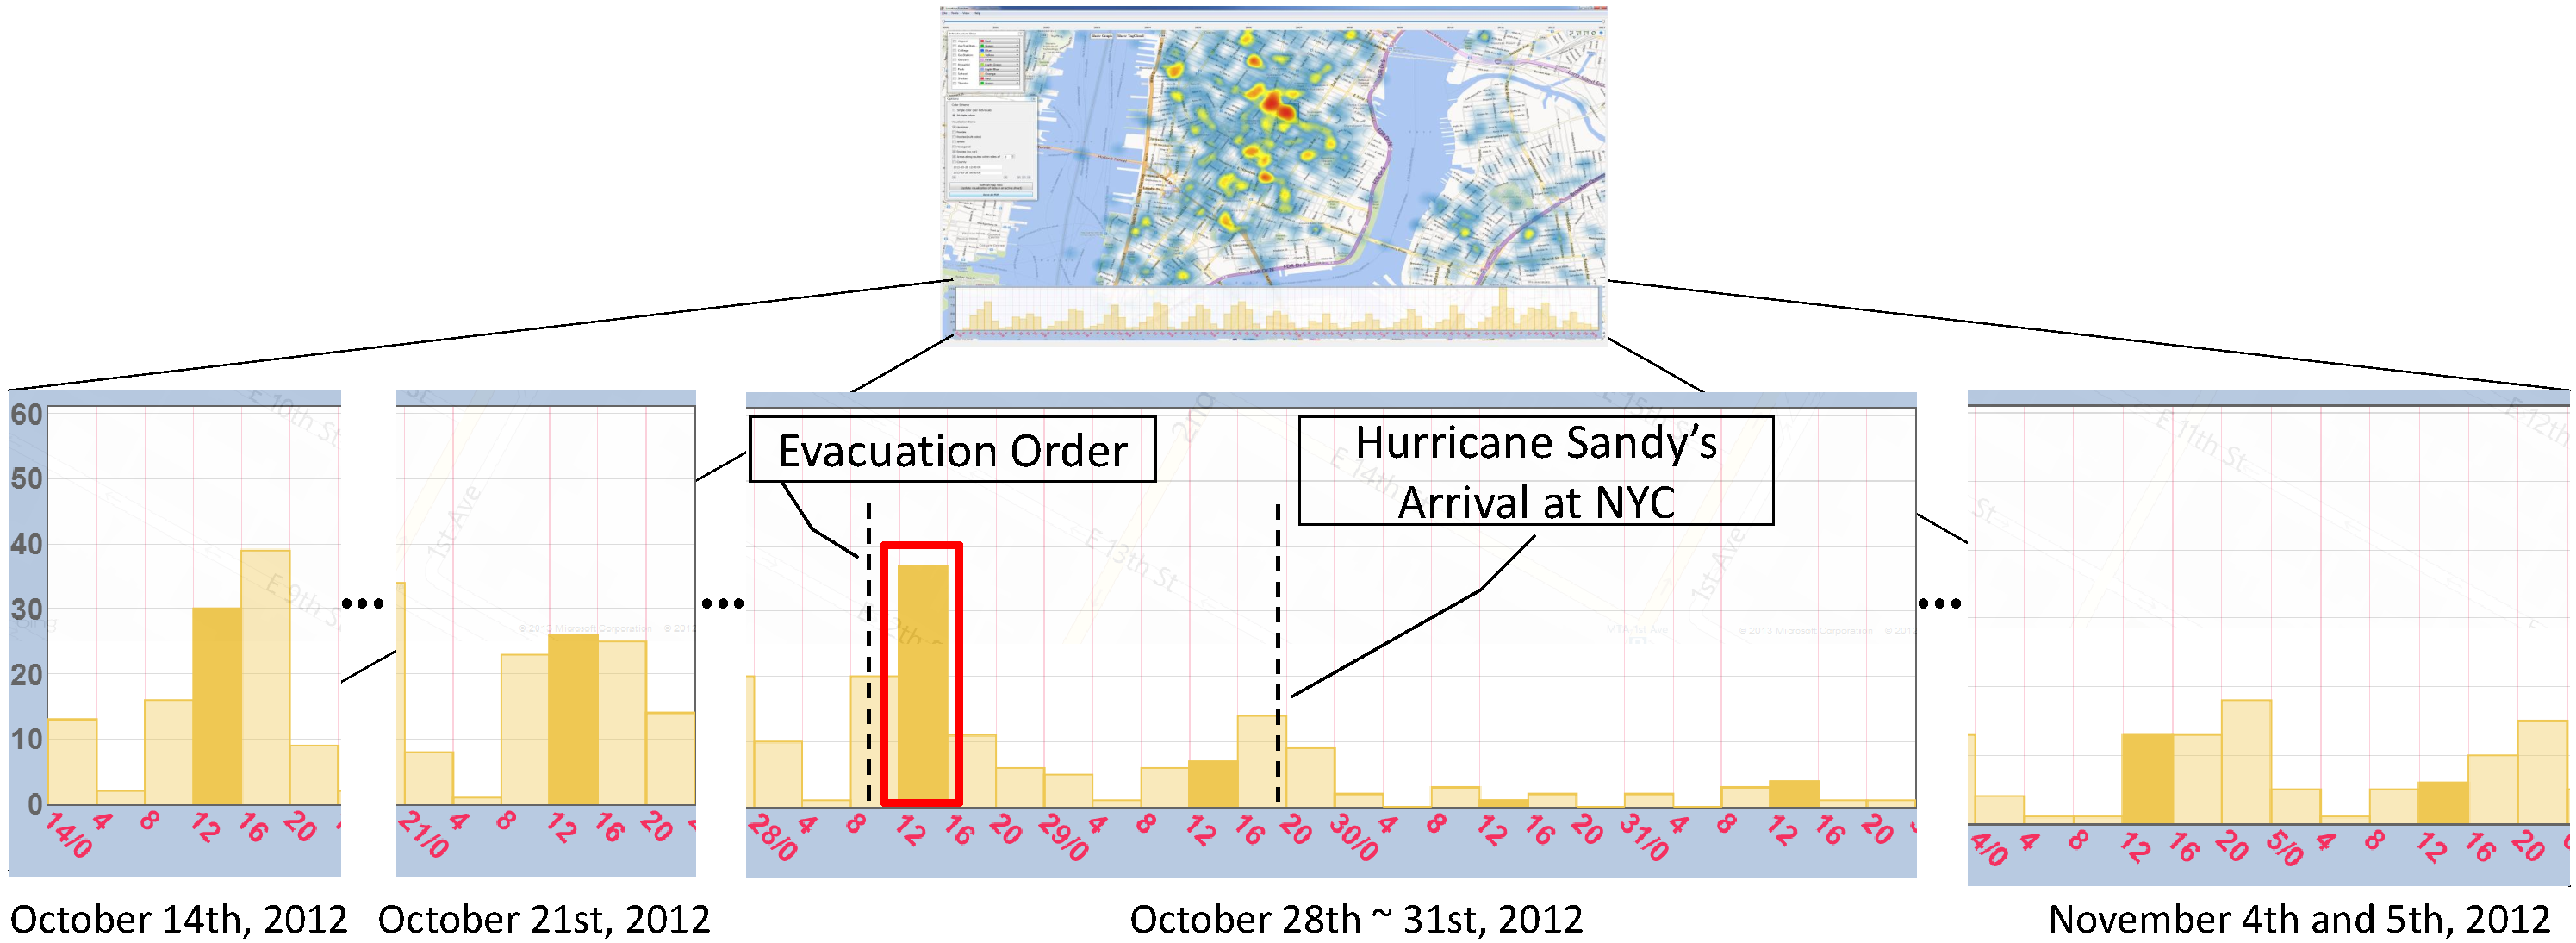
\includegraphics[width=0.80\linewidth]{graph_system_v4}
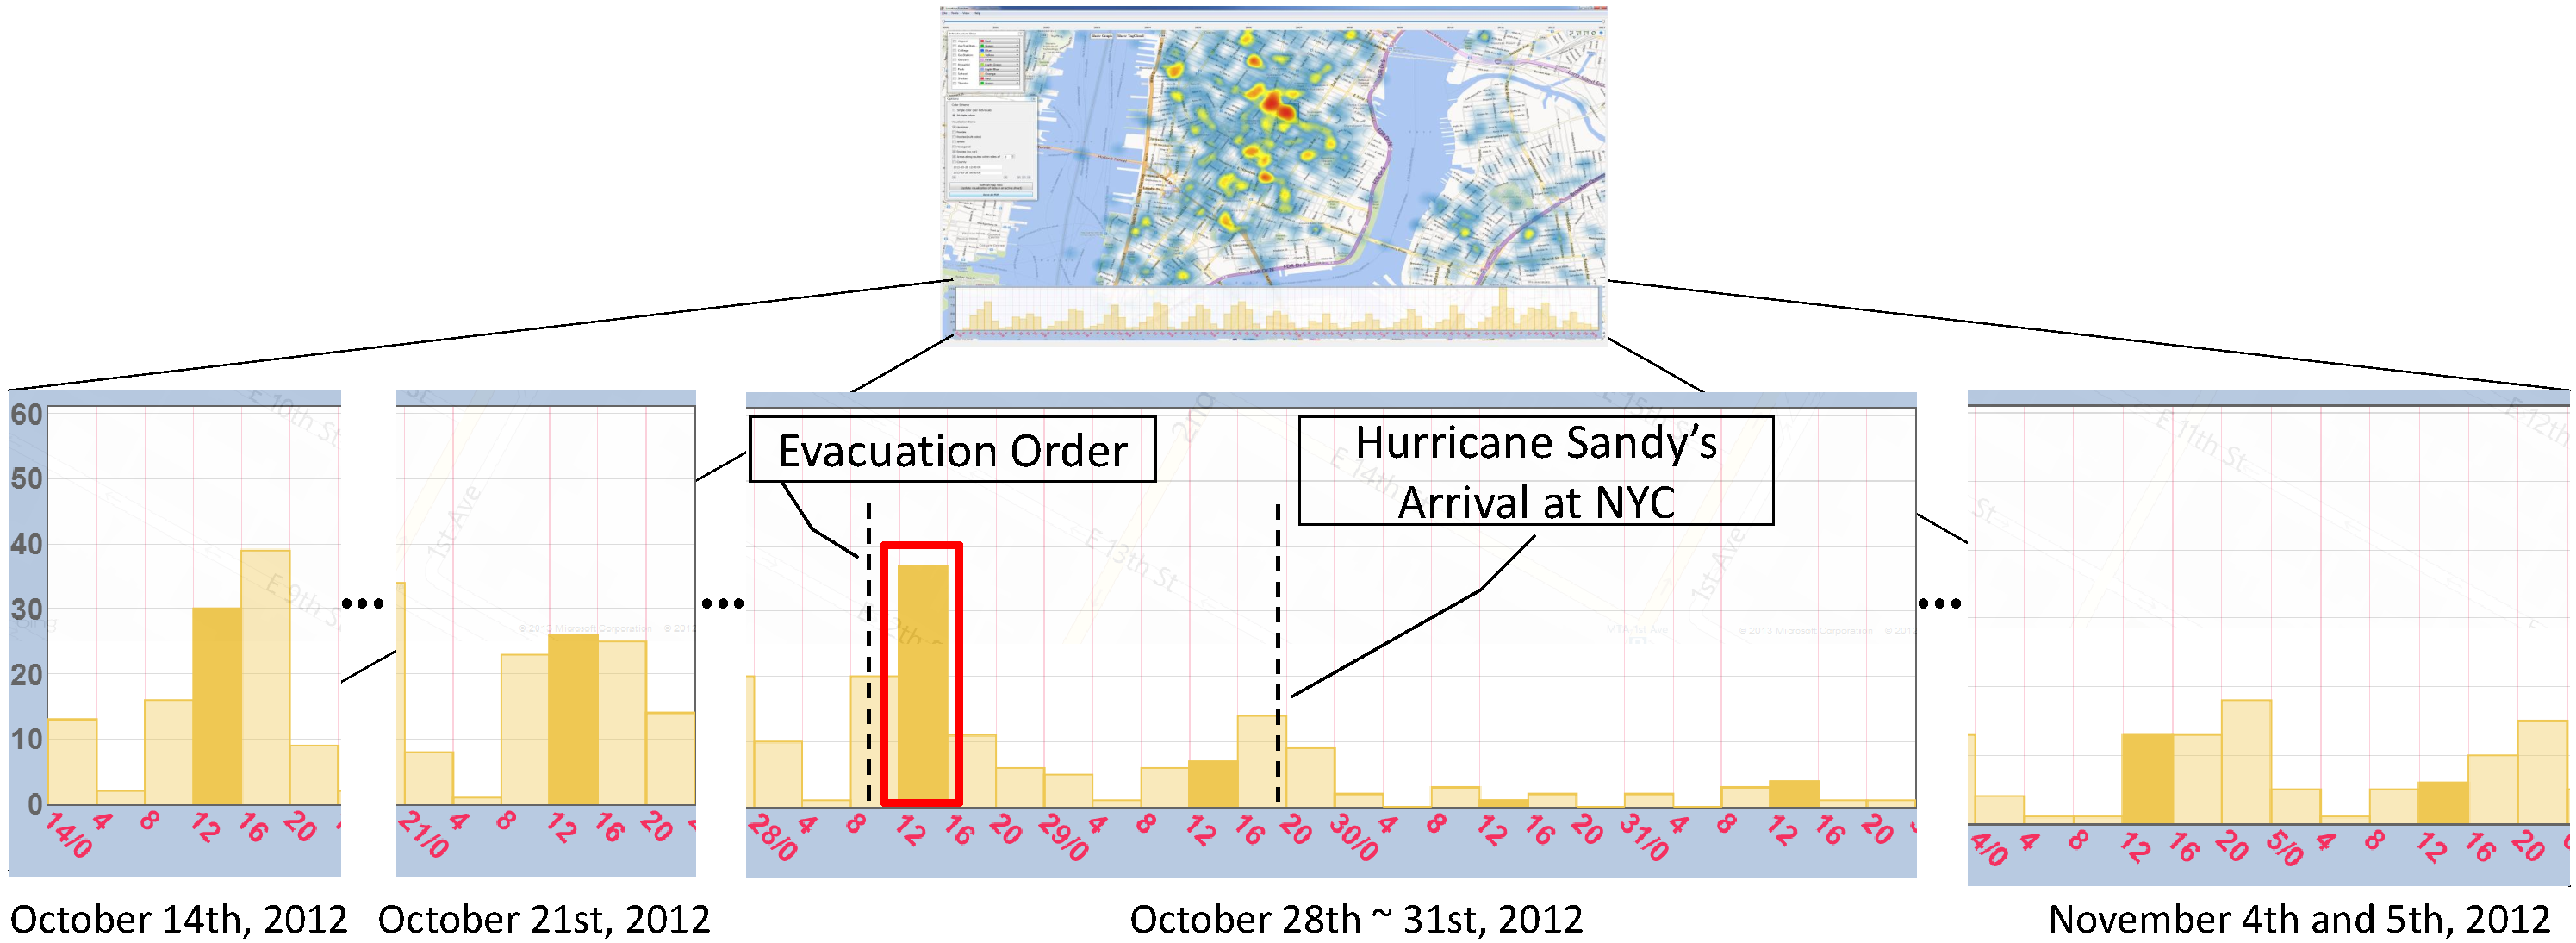
\includegraphics[width=1.0\linewidth]{graph_system_v4}
\caption{Temporal analysis for public behaviors during the disaster event, Sandy. Top shows our entire system view. 
The bar chart (Bottom) for the number of Twitter users within the selected region including a supermarket in Figure~\ref{fig:heatmap_manhattan} (Right) in four hour intervals is shown.
%some interesting time frames of the entire plot on the system. 
We see that many people went to the supermarket right after the evacuation order.}
\label{fig:graph}
%\vspace{-0.4cm}
\end{figure}





\subsection{Spatiotemporal Visualization}
\label{sec:spatiotemporal_visualization}

\begin{figure}[tb]
\centering
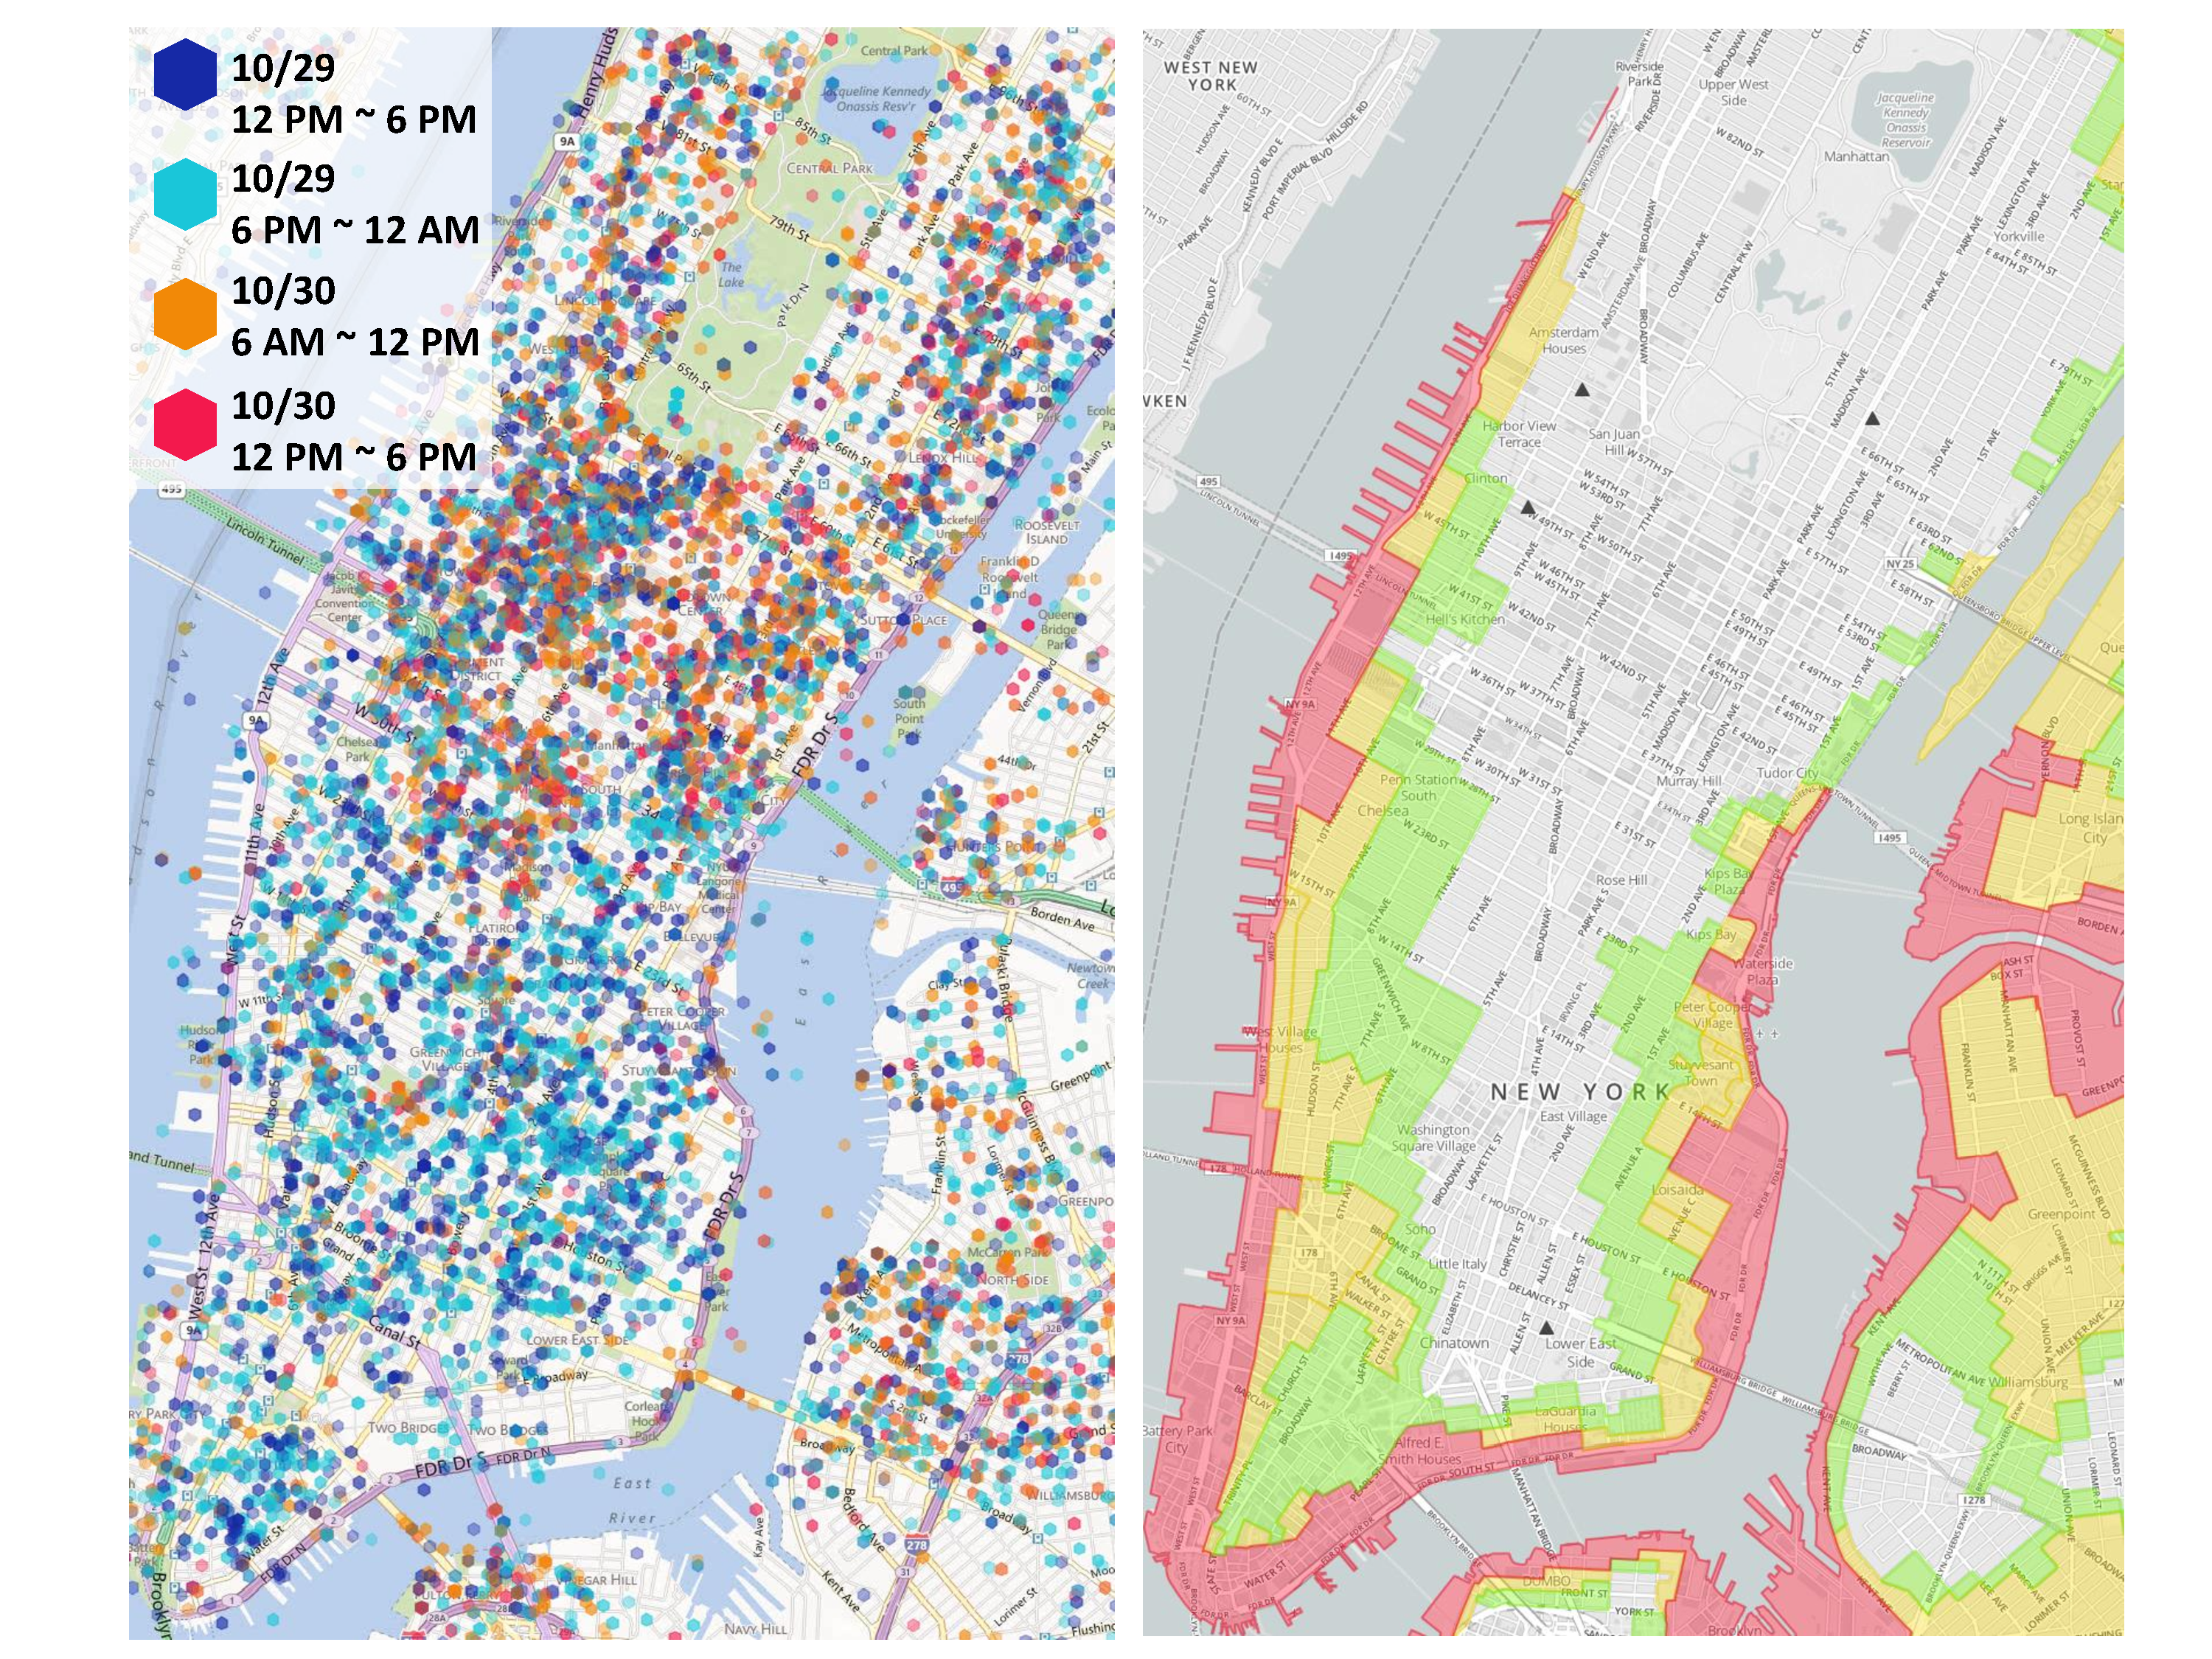
\includegraphics[width=1.0\linewidth]{spatiotemporal4}
\caption{Visualization for spatiotemporal social media data (Left).
A hexagon represents the spatial (position) and temporal (color) information of a Tweet.
Hurricane evacuation map~\cite{NYC:2012:HEM} (Right). Residents in Zone A (red) faced the highest risk of flooding, Zone B (yellow) and Zone C (green) are moderate and low respectively.}
\label{fig:spatiotemporal}
%\vspace{-0.8cm}
\end{figure}


There is abundant research published on the topic of spatiotemporal data visualization.
Still, exploration of time-referenced geographic data is still a challenging issue~\cite{Andrienko:2003:ESV}.
We introduce a modest visualization that enables analysts to analyze both aspects: space and time in a single view.
Each Tweet is independent and contains multiple properties, such as location, time, the number of re-Tweet, etc.
In this study, therefore, we utilize a glyph-based visualization to depict both location and time aspects of the independent data record using two visual features.
As shown in Figure~\ref{fig:spatiotemporal}~(Left), each hexagon corresponding to a Tweet represents the spatial and temporal information where the center of each hexagon is the location of each Tweet and the color represents its posting time.
In other words, space and time properties are encoded in a single visualization to harness the spatial analysis features of human visual perception~\cite{Treisman:1980:FIT}.
In Figure~\ref{fig:spatiotemporal}~(Left), the hexagons with blue~(12 PM $\sim$ 6 PM) or green~(6 PM $\sim$ 12 AM) ) color correspond to Tweets published on October 29th, 2012 and ones with orange or red color correspond to Tweets posted on the following day after the hurricane.
New York City announced the evacuation of Zone~A~(red color) in Figure~\ref{fig:spatiotemporal}~(Right); residents in Zone~A faced the highest risk of flooding, whereas, Zone~B~(yellow color) and Zone~C~(green color) are moderate and low respectively.
In the visual representation, analysts can indicate overall spatiotemporal patterns of people and their movements during the disaster event\textemdash many people still remained at home one day after the mandatory evacuation order, but most people left home on the following day as the hurricane damaged the city.
%\vspace{-0.3cm}

\section{Discussion and Evaluation}
\label{sec:discussion}
%
In this work we found out that the public responses to disaster events in social media streams are different according to the disaster event types.
Hurricane Sandy had a long time duration\textemdash more than one week, and affected a wide range of areas.
Therefore, there were many reactions in the potential damage area before the hurricane impacted the area.
%We could also indicate some hotspots in the area during the event.
However, no or significantly less hotspots were found right after the hurricane passed over the area.
This was because the hurricane severely affected the areas\textemdash communication facility damage and power outages occurred in the area.
Moreover, we found out that unusual post-event situations in the Twitter user distribution continued for a certain time period from a couple of days to more than one week as shown in Figure~\ref{fig:east_coast} and~\ref{fig:graph}.
%~\ref{fig:atlantic_coast}.
The analysts could estimate how long it took for the reconstructions in the areas.
%Hurricane-force winds can extend outward to about from 25 miles to more than 300 miles from its center.

Regarding the tornado case, we intended to find abnormal patterns in the Twitter user distribution before and during the disaster event
but there was no unusual patterns in the area.
In contrast to the hurricane, the tornado generally affected the areas relatively shortly, for example, a few minutes to an hour.
The abrupt natural disaster did not strongly influence the social media stream before and even during the event.
However, as shown in Figure~\ref{fig:tornado}, we were able to find many hotspots within the damaged areas after the tornado passed.
In fact, the tornado damaged some small areas (i.e., a couple of miles wide), in contrast to the wide range of damaged areas for the hurricane case.
This indicated that communication facilities were still available and many people were interested in the disaster, similar to the hurricane.
Thus, our social media analysis could support the analysts to make plans and manage for the emergent situations according to the types of the disasters.
%The number of Tweets are very different between rural and urban areas.

The above cases demonstrate how our system supports spatial decision making through evaluation of varying-density population area to determine changes in behavior, movement, and increase overall situational assessment. This increased spatial activity and behavioral understanding provides rapid situational assessment and provides insight into evolving situational needs to provide appropriate resource allocation and other courses of action (e.g., traffic rerouting, crowd control).

%There is a use case scenario of disaster management support utilizing our visual analytics system.
%Analysts can locate the high density population spots and understand the local situations using our system before or during a disaster event. 
%Then, they can quickly and appropriately respond, such as traffic control to the situations or resource allocation in order to mitigate potential risks.
We requested informal feedback for the usability of our system from users within our universities, and received useful and positive comments and suggestions.
They were interested in the findings of the abnormal situations during the disaster events in Section~\ref{sec:spatial_analysis} and~\ref{sec:temporal_pattern}. They also noted that the use of the infrastructure symbols on the heatmaps improved the legibility of the Twitter user distributions in Figure~\ref{fig:heatmap_manhattan}
and they suggested a visualization for the deviations between multiple heatmaps in order to show the differences clearly, which we plan to develop in the future.
%Furthermore, we are planning to conduct a formal experiment for user evaluation for our system in the future.
%Our system provides a testbed for evaluating the impact of interactive spatiotemporal visual analytics using social media data in disaster management.
%Furthermore, we are planning to conduct a formal user evaluation for 
%the impact of interactive spatiotemporal visual analytics using social media data on disaster management.
%We plan to evaluate: (1) the effect of geospatial visual support to explore and examine public spatial distribution using microblog data; (2) the effect of supplementary spatial information support for spatial decision-making (vs. without any supplementary information); (3) the usability of the glyph-based spatiotemporal visualization; and (4) the performance of the system under different locations, different types of disasters, and different location-based social media data.

%\begin{itemize}
%\item the effect of having geospatial visual support for exploring and examining public spatial distribution using microblog data;
%\item the effect of supplementary spatial information support for spatial decision-making (vs. without any supplementary information);
%\item the usability of the glyph-based spatiotemporal visualization;
%\item and the performance of the system under different locations, different types of disasters, and different location-based social media data.
%\end{itemize}


\section{Summary}
\label{sec:conclusions}
%
In this work we presented a visual analytics system for public behavior analysis and response planning in disaster events using social media data.
We proposed multiple visualizations of spatiotemporal analysis for disaster management and evacuation planning.
For the spatial decision support, we demonstrated an analytical scheme by combining multiple spatial data sources.
Our temporal analysis enables analysts to verify and examine abnormal situations.
Moreover, we demonstrated an integrated visualization that allows spatial and temporal aspects within a single view.
We have still some limitations with these techniques including the potential occlusion issues in the spatiotemporal visualization.
%For future work, we will investigate the flow of public movement before and after disasters and the analysis for recovering from disasters and crises. We also plan to design the glyphs with varied sizes adapting to the zoom level in the spatiotemporal visualization. 
%In addition, 
%%we will conduct a user evaluation of our system in the future.
%we will conduct a user evaluation for the usability and effectiveness of the geospatial visual support,
%and the impact of interactive spatiotemporal visual analytics using social media data on disaster management.
%, the effect of supplementary spatial information support for spatial decision-making (vs. without any supplementary information); (3) the usability of the glyph-based spatiotemporal visualization; and (4) the performance of the system under different locations, different types of disasters, and different location-based social media data.


%This system provides a heat map of people who posted geo-located Tweets around the Manhattan area during specific time periods and allows us to analyze their spatial distribution.
%Our bar chart visualization enables users to analyze the temporal distribution of the number of people tweeting in a given location and time.
%Finally, we provide a visualization that allows users to simultaneously analyze both aspects: space and time using a single view.

%The remainder of this document is structured as follows: 
%Section~\ref{sec:relatedwork} is a review of related work.
%We demonstrate how to improve investigations and analysis for public behavior response to the disaster by spatiotemporal analysis of social media in Section~\ref{sec:body}.
%Finally, we present a conclusion and future work in Section~\ref{sec:conclusions}.

%\subsection{Data and Event}
%\label{sec:data}
%
%\begin{figure}[tb]
%\centering
%\includegraphics[width=0.9\columnwidth]{Sandy_Track}
%\caption{Track of Sandy}
%\label{fig:sandy_track}
%%\vspace{-0.8cm}
%\end{figure}
%
%Explain about data and events

\chapter{Trajectory-based Visual Analytics for Anomalous Human Movement Analysis}

Analysis of human mobility patterns is important for urban planning, traffic forecasting, and understanding the pandemic spread of diseases.
%Even though human movements are free, their patterns can exihibit a high degree of spatiotemporal regularity and can exhibit structure~\cite{Gonzalez:2008:UIH}.
For crisis and disaster events, movement analysis, such as where people move to/from and how people respond to disasters, is also critical for evacuation management.
Unfortunately, finding meaningful data is challenging and collecting relevant data can be costly.
%show common structured patterns.
However, the rapid development and increasing availability of mobile communication and location acquisition devices allow people to share location data using existing social networks.
These LBSNs have been gaining attention as promising data sources for analyzing human movements.
%and have beneficial characteristics: easy access, the large volumes, and a variety of information.
Particularly, trajectories\textemdash sequences of geo-referenced data nodes of each user\textemdash extracted from such LBSNs provide opportunities and solutions to challenges in human movement analysis~\cite{Andrienko:2009:Analysis, Fuchs:2013:Extracting, Gabrielli:2014:Tweets}.
Also, LBSNs play an important role in the way people act and react to the world, not only in daily life, but especially during abnormal situations.
In emergency situations, people interact with others through LBSNs to confirm information and obtain situational awareness of the potential risks~\cite{national:2013:Public}.
%In addition, LBSN services provide multiple types of semantic context information.
In addition, their semantic context enhances understanding of local events and human movements~\cite{Hochman:2012:Visualizing, Zin:2013:Knowledge}.
%Vrotsou:2012:Interactive

Previous studies have mainly focused on finding regular movement patterns using spatial data.
They have demonstrated that human movements are normally influenced by geographic constraints, life patterns, and spatial and temporal events, such as local festivals and holiday seasons~\cite{Andrienko:2011:Movement, Fujisaka:2010:DOU}.
%However, the research may have limitations.
However, during disaster events, since human movement patterns (e.g., volume and direction of movements) are unusual compared to normal situations, a new approach is required to analyze the movements.
Also, analyzing location data alone has shown limitations in achieving situational awareness of local events.
For example, they cannot answer why people move and what situations occur.

To address these challenges, we propose a trajectory-based visual analytics system for anomalous human movement analysis during disasters using multi-type online media.
We extract trajectory using Tweets with geo-location, and geo-tagged photographic data from Instagram (a photo sharing social network service).
Our system generates trajectories using geo-location information of chronologically ordered Tweets for each person.
The extracted raw trajectories, however, do not have enough fine-grained spatial positions.
We supplement the sparse positions in the trajectories using route information between each position.
%The complemented trajectories are visualized for further examinations.
We group the individual trajectories into classes of similar sub-trajectories using a trajectory clustering model based on the partition-and-group framework~\cite{Lee:2007:Trajectory}.
This enables users to discover sub-common patterns, rather than finding common patterns as a whole.
%even though there is no common pattern if the basic unit of clustering is the whole trajectory.
%Our system allows users to track and examine change of movement patterns over time.%: past and current.

We also propose a classification model based on historical data for abnormal movement detection using human expert interaction.
We allow users to utilize their domain knowledge of the spatiotemporal characteristics of their regions of interest to interactively identify and compare abnormal trajectory patterns with normal trajectory patterns.
%We expect the users of our system have knowledge about geographical and temporal characteristics of the location where an abnormal event of interest occurred.
%The users select a target time window or a real time mode for the abnormal situation and also choose another time window representing a normal situation.
%We extract two sets of trajectories for the two different time windows.
%Our analytics model then identifies abnormal movement patterns based on the movements of the normal situation.
In addition, we integrate multiple visual representations using relevant context extracted from different online media sources, such as Tweet text, shared photos, public webcam videos, and news media to allow users to discover and analyze anomalous human movement patterns; thereby, improving situational awareness in disaster management situations. 
%This enhances the human movement analysis by improving situational awareness.
%In addition, based on the discovered movements, we extract multiple types of semantic context information (i.e., photo, video, news media) from different data sources and then visually incorporate the information into the system
%Through case studies, we demonstrate how our analytics model discovers anomalous human movement patterns during crisis events and how our visual analytics system improves the movement analysis for disaster management.

The major contributions of this work are as follows:
\begin{itemize}
\item We develop a visual analytics system to discover and explore common structural movement patterns from unstructured massive movement data.
%\item We provide a visualization scheme that allow the analysts to simultaneously analyze trajectory patterns over different time frames.
%\item We design a trajectory-based anomaly detection model to detect and track abnormal human movement patterns.
\item We design a trajectory-based classification model for abnormal movement detection using human expert interaction.
\item We develop visual means to improve human movement analysis using semantic context available from multiple online media sources.
%\item We develop visual means to improve human movement analysis by combining an exploratory spatiotemporal analysis of trajectories with semantic context information available from multiple types of social media.
\item We demonstrate the effectiveness of our system in disaster management and evacuation planning through case studies.
\end{itemize}


\section{System Overview}

Our system is designed for exploring and discovering common movement patterns and detecting abnormal situations using LBSN data. The system consists of four major components: a trajectory extraction module, a data analysis module, a context extraction module, and a visualization module as illustrated in Figure~\ref{fig:process}.
%Users first apply a spatiotemporal filter of interest into the system.
%Users select an area and a target time window of interest or a real time mode.
%The users then specify one or multiple past time windows representing normal situations compared to the target time frame.
%We assume that the additional time frames represent normal situations.
The \textit{trajectory extraction module} (Section~\ref{sec:trajectory_extraction}) generates two different sets of trajectories: target and normal trajectories.
%with geo-location information extracted from tweets and Instagram data filtered by the sptiotemporal filter.
The \textit{data analysis module} (Section~\ref{sec:analysis_models}) consists of two components: common movement discovery and abnormal pattern detection. 
For the given trajectory sets, the first component discovers major common routes based on the partition-based clustering model, and the other component assesses the abnormality for each common route.
%More details will be described in Section~\ref{sec:analysis_models}.
\begin{figure}[hbt]
\centering
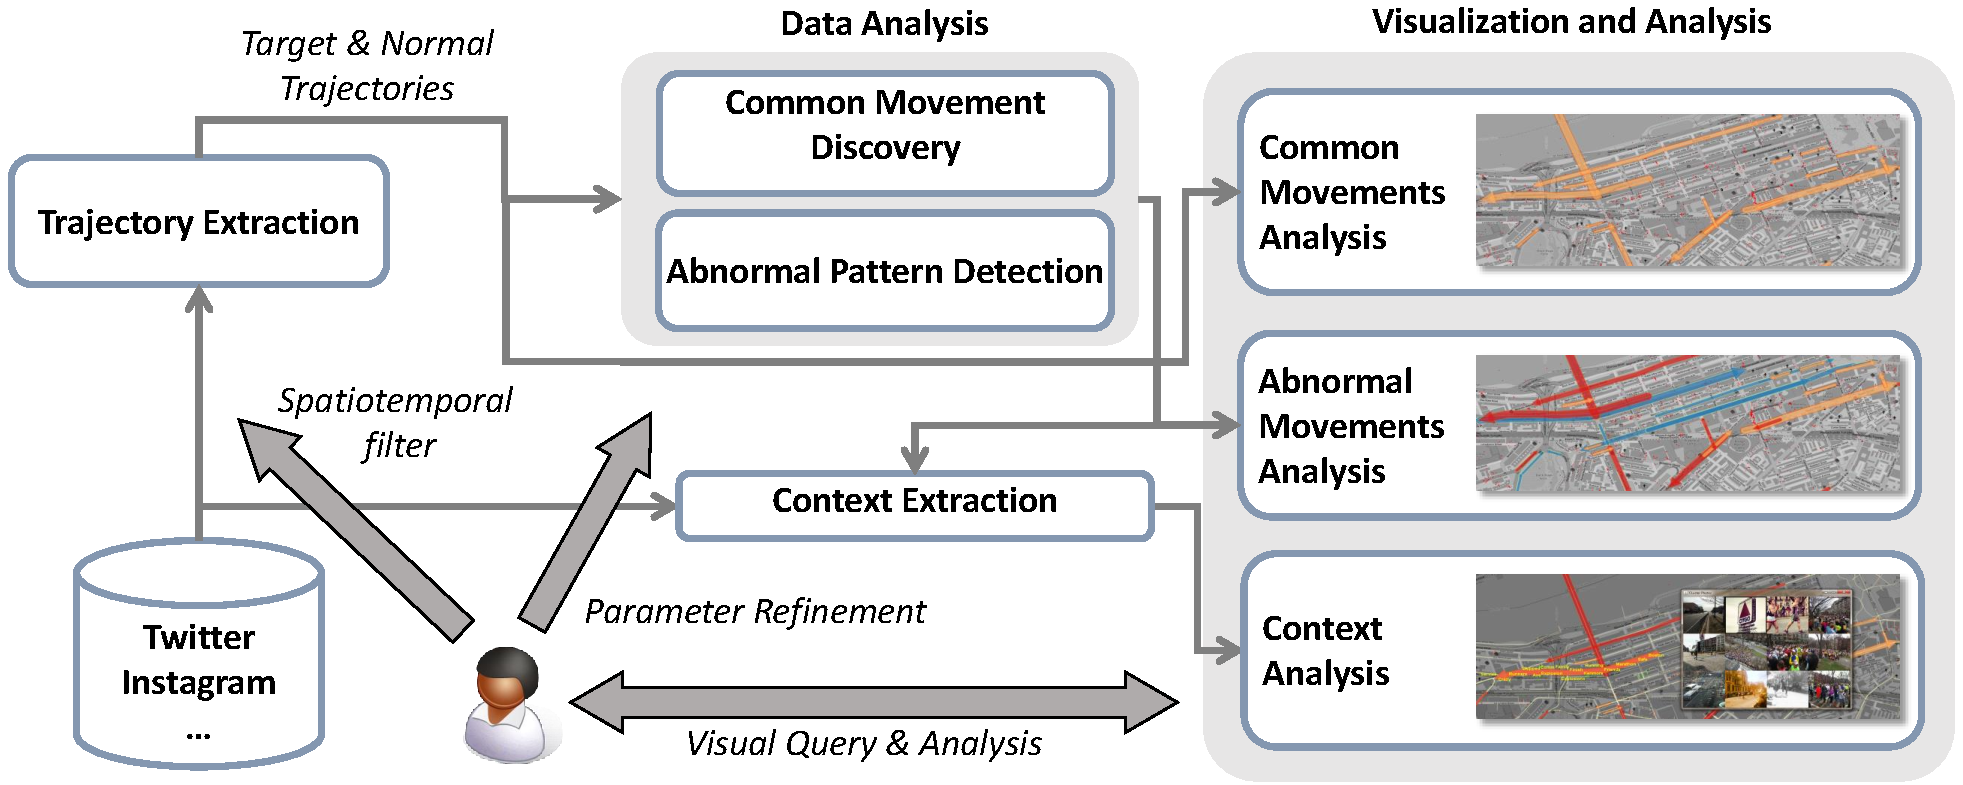
\includegraphics[width=1.0\linewidth]{process_v3}
\caption{Overview of our iterative analysis scheme for human common movement discovery and anomaly analysis.}
\label{fig:process}
%\vspace{-0.4cm}
\end{figure}
The \textit{context extraction module} (Section~\ref{sec:context}) finds relevant context information including keywords, photos, videos from web cameras, and news media based on the results from the analysis module.
The \textit{visualization module} (Section~\ref{sec:visualization}) allows the users to explore the trajectories, common routes, and abnormal movements, and obtain a better understanding of movement patterns using additional context.
Users can iteratively make visual queries and refine the parameters used for clustering and anomaly detection to optimize the results.
\subsection{Trajectory Extraction}
\label{sec:trajectory_extraction}

Our system extracts trajectories from location-based social media data.
Users first select a geographical boundary and a target time window of interest.
% or a real time mode.
The users additionally select one or more past time windows representing normal situations to compare against the target time frame.
The trajectory extraction module then requests two sets of Tweets from the database for the two selected time windows.
%Two sets of the tweets generated within the each time windows.
The module generates two sets of trajectories: target and normal trajectories using geo-location information of chronologically ordered Tweets for each person.

\begin{figure}[tbh]
	\centering
	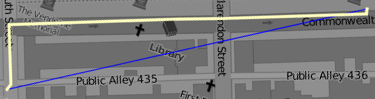
\includegraphics[width=0.8\linewidth]{route_v2}
	\caption{Supplementing a sparse trajectory (Blue) using route direction information (Yellow). }
	\label{fig:route}
	%\vspace{-0.4cm}
\end{figure}

%The extracted raw trajectories, however, do not have enough fine-grained spatial positions.
The generated trajectories, however, are usually sparse and incomplete.
%compared to ones generated by GPS devices (the interval is a couple of seconds between each point).
For example, as shown in Figure~\ref{fig:route}, the sparse trajectory (a blue line) does not represent a realistic movement.
In order to reduce the spatial sparseness of the raw trajectories, 
we fill the trajectories with supplementary points between two points for each pair of the trajectories, which are calculated by shortest-path-based route directions (a yellow poly line in Figure~\ref{fig:route}).
%We compensate the sparse positions in the trajectories using route information between each position.
%In this work, we use geo-location information extracted from tweets to build trajectories of each user.
%However, the temporal intervals between each posting have a high degree of variation\textemdash a couple of from minutes to hours.
%Therefore, it is hard to find realistic movements using the high sparse trajectories.
%The abstraction level of the trajectories is too high to obtain actuality.
%We need appropriate fine-grained spatial positions between the recorded positions.
In this work, we use the Bing Maps API to obtain route information.
We can choose one of the following travel modes: walking, driving, or public transportation mode depending on the location and the situation.
For example, we select the walking mode for the Boston Marathon case because many traffic routes along the marathon course were closed on the race day.
%The Google Maps API also provide a route calculation service, but for the public license users, the number of requests is limited.

%\begin{itemize}
%\item Finding references showing how much the shortest route is similar to the real movement
%\end{itemize}
\subsection{Data Analysis}
\label{sec:analysis_models}
In this section we describe the data analysis module.
This module analyzes the trajectories given by the trajectory extraction module.
%This module consists of two components: common movement discovery and abnormal pattern detection.
The following sub-sections provide the details of this module.

\subsubsection{Common Movement Discovery}
\label{sec:common_movement_discovery}
Discovering common movements is a critical process for exploration and analysis of a large volume of trajectory data.
%where the entities that need to be analyzed are trajectories.
Clustering is a popular approach in looking for common patterns in the trajectory data.
%by organizing trajectories into groups whose members are similar in some way.
%A number of clustering algorithms have been proposed by researchers.
Representative clustering algorithms for trajectory include DBSCAN~\cite{Ester:1996:Density} and OPTICS~\cite{Ankerst:1999:Optics}.
Andrienko et al.~\cite{Andrienko:2013:Visual} propose a wide range of clustering-based analytics models and combine those with visualization techniques.
Their clustering models, however, group similar trajectories as a whole and extract common whole trips.
In this work, we utilize a modified partition-based clustering model, TRACLUS~\cite{Lee:2007:Trajectory}, in order to find common sub-trajectories.
For each given trajectory, this model first partitions a trajectory into a set of line segments, and then groups the line segments into clusters of similar line segments.
Clustering the line segments (as opposed to whole trajectories) eables the extraction of similar portion of trajectories.
%Clustering the line segments is very useful, because we can extract common behaviors, even though there is no cluster if the basic unit of clustering is the whole trajectory.
For example, Figure~\ref{fig:common_sub_trajectory} shows that the three trajectories (green, black, red) have different origins and destinations, but there is a common path in all three trajectories (blue).
%This is valuable information.
%We need to discover the common behavior. This is valuable information.
%
%For trajectory partitioning, the existing model utilizes MDL~\cite{Grunwald:2005:Advances} to find characteristic points that change the direction rapidly from all points of each trajectory.
%In this work, however, the points resulting from the way are too spares to partition the trajectories into appropriate line segments.
%Therefore, we use the series of the waypoints resulting from the route direction calculation service described in Section~\ref{sec:trajectory_extraction} in order to gain adequately fine-grained characteristic points.
%, for example, the black dots of each trajectory in Figure~\ref{fig:common_sub_trajectory}.

\begin{figure}[tb]
	\centering
	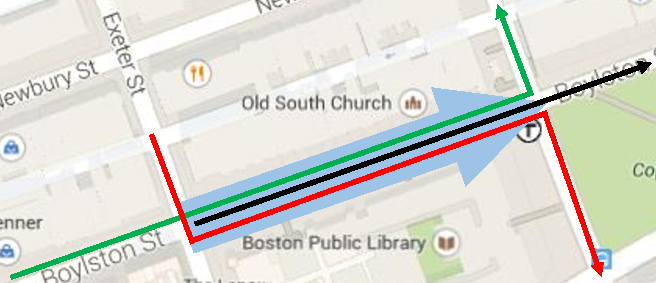
\includegraphics[width=0.8\linewidth]{common_sub_trajectory_v2}
	\caption{Discovering a common sub-trajectory.}
	\label{fig:common_sub_trajectory}
	%\vspace{-0.4cm}
\end{figure}

Clustering the line segments requires a distance function measuring the distance between line segments.
We use the distance function based on a modified line segment Hausdorff distance~\cite{Chen:2003:Noisy}, which is comprised of three components: the perpendicular distance ($d_\bot$), the parallel distance ($d_\parallel$), and the angle distance ($d_\theta$).
Let $s_i$ and $e_i$ be the starting and ending points of line $L_i$, and $s_j$ and $e_j$ for line $L_j$.
Without loss of generality, the longer line segment is assigned to $L_i$, and the shorter one to $L_j$.
These are illustrated in Figure~\ref{fig:distancefunction}.

For our distance function, we use $d_\bot$ and $d_\parallel$ as defined by ~\cite{Chen:2003:Noisy}, but redefine $d_\theta$ as the existing model does not consider the directions of the two line segments for the angle distance measure.
In this work direction is an important factor in clustering and abnormal movement detection.
To consider the direction, we utilize the cosine-similarity that measures the cosine of the angle between line segments, and is used as a bounded similarity function within $[0,1]$. 
$d_\theta(L_i, L_j)$ is defined as:
%This is different from ~\cite{Lee:2007:Trajectory}.
%The angle distance:
\begin{equation}
\begin{aligned}
d_\theta(L_i, L_j) = \parallel L_j \parallel \times \frac{\cos^{-1} (\mathit{cosine\mbox{-}similarity}(L_i, L_j))} {\pi}
\end{aligned}
\end{equation}
where $\parallel L_j \parallel$ denote length of $L_j$, and $\theta$ $(0^{\circ} \le \theta \le 180^{\circ})$ denote the smaller intersecting angle between $L_i$ and $L_j$, and $\mathit{cosine\mbox{-}similarity}(L_i, L_j)$ is defined as:
\begin{equation}
\mathit{cosine\mbox{-}similarity}(L_i, L_j) = \cos (\theta) = 
\frac{\overrightarrow{s_i e_i} \cdot \overrightarrow{s_j e_j} } {\parallel \overrightarrow{s_i e_i} \parallel \parallel \overrightarrow{s_j e_j} \parallel}	
\end{equation}
$\parallel L_j \parallel$ denote length of $L_j$, and $\theta$ $(0^{\circ} \le \theta \le 180^{\circ})$ denote the smaller intersecting angle between $L_i$ and $L_j$.


%The perpendicular distance:
%\begin{equation}
%d_\bot(L_i, L_j) = \frac{l_{\bot1}^2 + l_{\bot2}^2}{l_{\bot1} + l_{\bot2}}
%\end{equation}
%where $p_s$ and $p_e$ are the projection points of the points $s_j$ and $e_j$ onto $L_i$, respectively. 
%$l_{\bot1}$ is the Euclidean distance between $s_j$ and $p_s$; $l_{\bot2}$ is that between $e_j$ and $p_e$.
%
%The parallel distance:
%\begin{equation}
%d_\parallel(L_i, L_j) = MIN(l_{\parallel1}, l_{\parallel2})
%\end{equation}
%where $l_{\parallel1}$ is the Euclidean distances of $p_s$ to $s_i$ and $l_{\parallel2}$ is that of $p_e$ to $e_i$.

%where
%\begin{align*}
%\mathit{cosine\mbox{-}similarity}(L_i, L_j) = \cos (\theta) = 
%\frac{\overrightarrow{s_i e_i} \cdot \overrightarrow{s_j e_j} } {\parallel \overrightarrow{s_i e_i} \parallel \parallel \overrightarrow{s_j e_j} \parallel}	
%\end{align*}

%\begin{equation}
%\begin{aligned}
%d_\theta(L_i, L_j) = \parallel L_j \parallel \times \frac{\cos^{-1} (\mathit{cosine\mbox{-}similarity}(L_i, L_j))} {\pi}, \enspace \mathrm{where} \\
%\mathit{cosine\mbox{-}similarity}(L_i, L_j) = \cos (\theta) = 
%\frac{\overrightarrow{s_i e_i} \cdot \overrightarrow{s_j e_j} } {\parallel \overrightarrow{s_i e_i} \parallel \parallel \overrightarrow{s_j e_j} \parallel}	
%\end{aligned}
%\end{equation}


The distance function is finally defined as the sum of three components:
\begin{equation}
\label{eq:distancefunction}
\begin{aligned}
dist(L_i, L_j) = w_\bot \cdot d_\bot(L_i, L_j) + w_\parallel \cdot d_\parallel(L_i, L_j) + w_\theta \cdot d_\theta(L_i, L_j)
\end{aligned}
\end{equation}
where $w_\bot$, $w_\parallel$, and $w_\theta$ are weight values, which are determined depending on applications.

\begin{figure}[tb]
	\centering
	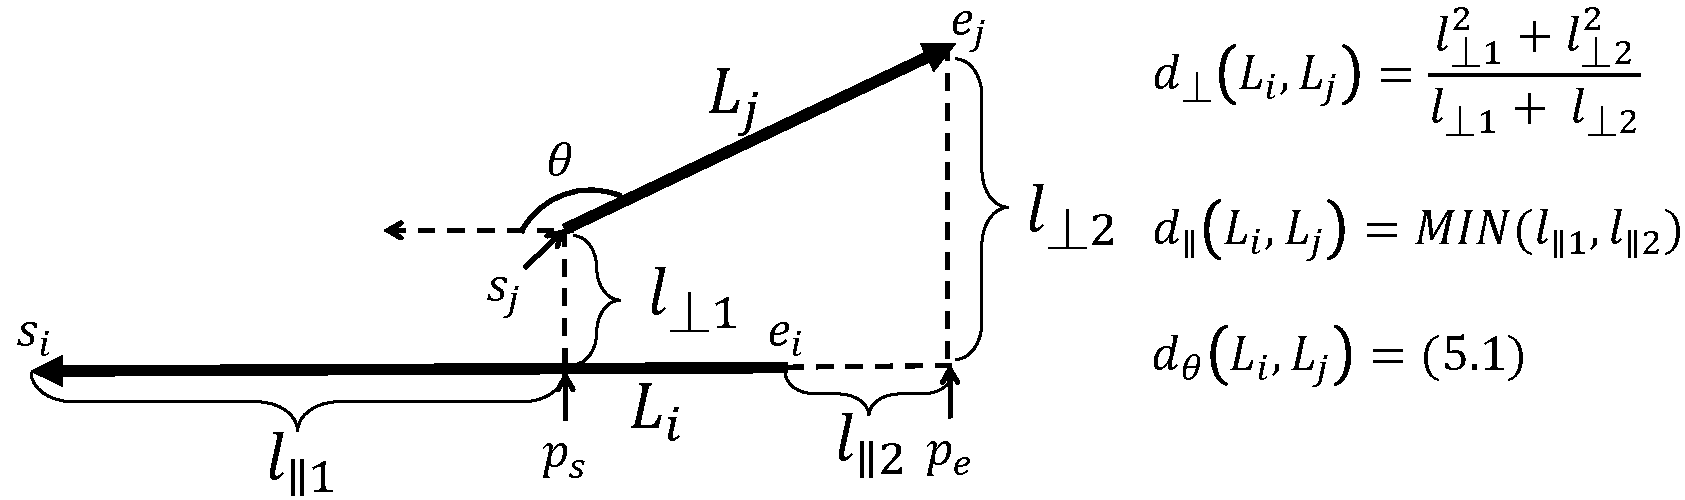
\includegraphics[width=1.0\linewidth]{distancefunction_v3}
	\caption{Similarity measurement for two line segments.}
	\label{fig:distancefunction}
	%\vspace{-0.4cm}
\end{figure}

The partition-based clustering model utilized in this work is based on the algorithm DBSCAN~\cite{Ester:1996:Density}.
Given a set of line segments, the algorithm groups the line segments into a set of clusters according to the distance function Equation (\ref{eq:distancefunction}).
DBSCAN requires two parameters: $\epsilon$ (as neighborhood distance) and $MinLns$ (as minimum cluster size).
The clustering model estimates the optimal parameter values based on input data.
An initial result generated by the estimated parameters is given to users.
However, the automatically estimated parameter values do not always provide optimal results.
Especially, $MinLns$ relies on user's domain knowledge and application requirements.
So, our system allows the users to manually adjust the estimated values.
The system then generates a representative trajectory for each cluster, which epitomizes the line segments (sub-trajectories) belonging to the corresponding cluster. More detailed information about these procedures can be found in ~\cite{Lee:2007:Trajectory}.


\subsubsection{Abnormal Movement Detection}
\label{sec:abnormal_movement_detection}
Existing anomaly detection models~\cite{Liao:2010:Anomaly,Lee:2008:Trajectory} for trajectory data have mainly focused on identifying outliers from a target dataset.
The models are usually based on non-supervised learning\textemdash they generally do not have factors for the outliers, and assume that the outliers make for a small sub-set from the entire dataset.
These models first look for major flow patterns and then determine whether each trajectory belongs to the majority according to specific criteria.
However, during abnormal situations, such as natural disasters and crisis events, even the major behaviors can be unusual compared to normal situations.

In this work, we propose a classification model based on historical data for abnormal movement detection using human expert interaction.
We allows the users to utilize their domain knowledge of the geographical and temporal characteristics of the location where an abnormal event of interest occurs.
The users select a target time window for the abnormal situation and also chooses another time window representing a normal/regular situation for the location.
%We expect the users of our system have knowledge about the location that need to be analyzed, such as regular or special events and temporal characteristics the location.
%We combine such human expert knowledge with our analytics model to detect abnormal movement.
%Our system requires not only a target time window to be analyzed, but also a past time window representing a normal/regular situation of the location from the users for comparison between the two situations.
We extract two sets of trajectories for the two different time frames and cluster each set of trajectories into two sets of trajectory clusters.
Next, we generate two different sets of representative trajectories: target $T$ and comparable $C$.
A representative trajectory $RT_{ti} \in T$ is classified as an outlier if there is a close representative trajectory $RT_{ci} \in C$.
More specifically, we identify outlying line segments $L_{ti} \in RT_{ti}$~\cite{Lee:2008:Trajectory}, which are determined by the distance from neighboring $RT_{ci}$.
We define a representative trajectory $RT_{ci}$ is close to a line segment $L_{ti}$ if $\sum_{L_{ci} \in CRT_{c}} len(L_{ci}) \leq len(L_{ti}) $ where $CRT_{c}$ is the set of $RT_{ci}$'s line segments within the distance $D$ from $L_{ti}$, $\left\{L_{ci} \enspace| \enspace dist(L_{ci}, L_{ti}) \leq D\right\}$. 
A larger value of $D$ detects a smaller number of outliers, and a smaller value of $D$ a larger number of outliers.
Then, intuitively a representative trajectory $RT_{ti}$ is outlying, if the percentage of the total length of outlying line segments is more than $P$. The default value of $P$ is set to 30.
Finally, the outlying representative trajectories are visualized.
Our system allows the users to adjust the two parameter values, $D$ and $P$ in order to refine their results.




%\input{anomaly_model}
\subsection{Visualization and Analysis}
\label{sec:visualization}
In this section we describe our design goals.
We introduce the visualization module to show common and abnormal movement patterns discovered by the data analysis module.
To illustrate our method, we use the Tweets generated near the finish line of the Boston Marathon during first 24 hours after the two explosions on April 15, 2013.

\subsubsection{Design Rationale}
Our design goal is to show trajectories extracted from geo-tagged Tweets of each person.
Displaying the trajectories without grouping can also reveal new insights when users drill down to individual movements.
%A spatiotemporal filter are also required to focus on a specific spatiotemporal space.
However, when the number of trajectories shown over the map increases, visual clutter issues arise that hinder the discover of flow patterns.
To reduce clutter, we use a modified partition-based trajectory clustering model for discovering common sub-trajectory patterns~\cite{Lee:2007:Trajectory}.
%Since our trajectories are usually sparse and incomplete compared to ones generated by GPS devices (the interval is couple of seconds between each point), we need a diff
%However, clustering trajectories as a whole cannot discover similar portions of trajectories.
%Even though some portions of trajectories with a long path show a common behavior, the whole trajectories might not.
%The common sub-behavior is also valuable information.
The discovered common movements have multiple attributes to be analyzed, such as cluster size, direction, and length.
%These attributes need to be displayed.
The users need to not only identify abnormal movement patterns, but also understand how abnormal and normal movement patterns differ.
The required clustering level can also vary with the application.
So, we need to allow the users to adjust the clustering level.
%We also would like to display change of movement patterns over time.

\subsubsection{Visualization of Common Movements}

Figure~\ref{fig:clustering_process} shows the process of discovering common movement patterns.
If we display the raw trajectories, it is difficult to understand the realistic movement patterns because of the high degree of sparseness of the trajectories as shown in Figure~\ref{fig:clustering_process} (left).
Therefore, we reduce the sparseness of the raw trajectories using the method described in Section~\ref{sec:trajectory_extraction} and display the supplemented trajectory on the map with 30\% opacity in Figure~\ref{fig:clustering_process} (center).
%the trajectories with a higher opacity represent the routes used by a higher number of people.
%The supplemented trajectories represent more realistic human mobilities than the raw one.
Users are able to examine more realistic human mobilities with the supplemented trajectories rather than using the raw ones.
%The trajectories supplemented with route directions show more realistic trips (transparent yellow poly lines)  and enable users to examine individual movements, in which the lines with a higher opacity represent the routes used by a higher number of people.
%The users are able to intuitively select a specific area and a time period to focus on their interest.
%However, if the number of trajectories shown over the map increase, the users will encounter difficulty in analyzing movement patterns.
Next, we cluster the trajectories into sets of similar sub-trajectories and generate representative trajectories for each cluster as described in Section~\ref{sec:common_movement_discovery}.
The representative trajectories represent common movement behaviors in Figure~\ref{fig:clustering_process} (right).

\begin{figure}[hbt]
\centering
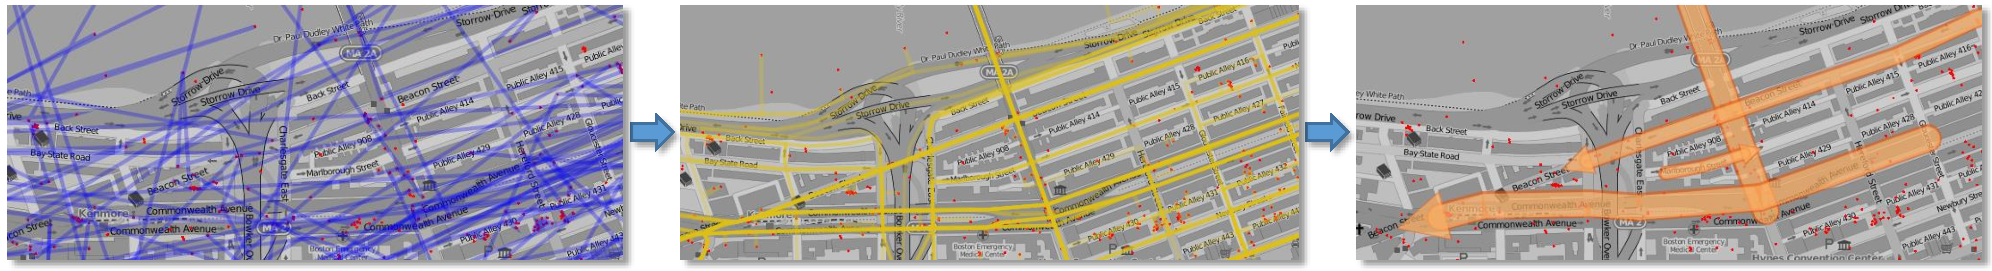
\includegraphics[width=1.0\linewidth]{clustering_process_v4}
\caption{The process of discovering common human movement patterns using location-based social networks data.
Visualization of sub-trajectory clusters (right). The thickness of each trajectory represents the size of the cluster.}
\label{fig:clustering_process}
%\vspace{-0.4cm}
\end{figure}

We provide visual cues to show multiple attributes for a representative trajectory.
We use a poly line with an arrow head to display the length and the direction of the representative trajectory.
The thickness of the line represents the size (i.e., the number of sub-trajectories belonging to a cluster) of the corresponding cluster.
Figure~\ref{fig:cluster_properties} shows the representative trajectories within the region same as the one in Figure~\ref{fig:clustering_process} (right).
Placement order of the trajectories depends on the length; the longest trajectory is placed at the bottom and the shortest one at the top, to avoid obscuring the shorter trajectories.

Our system also enables users to adjust and refine the $\epsilon$ (as neighborhood distance) and $MinLns$ (as minimum cluster size) values used by the clustering algorithm depending on their requirements by visual inspection.
We display an initial clustering result calculated with the automatically estimated parameter values as described in Section~\ref{sec:common_movement_discovery}.
The optimal result in Figure~\ref{fig:clustering_level} (top) is achieved at $\epsilon=25$ and $MinLns=3$.
The algorithm generates a larger number of smaller clusters, when $\epsilon$ is smaller or $MinLns$ is larger compared to the optimal values.
In contrast, the algorithm generates a smaller number of larger clusters when $\epsilon$ is larger or $MinLns$ is smaller.
For example, the result at $\epsilon=25$ and $MinLns=4$ is shown in Figure~\ref{fig:clustering_level} (center) and the results at $\epsilon=30$ and $MinLns=2$ is shown in Figure~\ref{fig:clustering_level} (bottom).

\begin{figure}[tb]
	\centering
	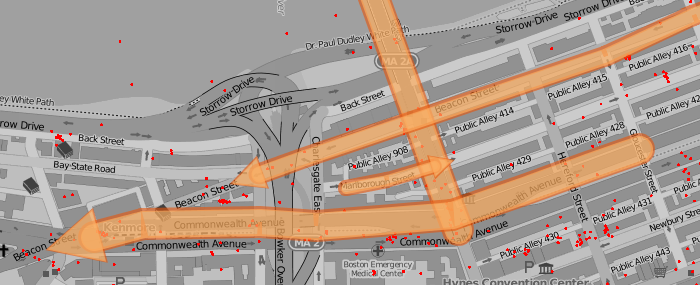
\includegraphics[width=1.0\linewidth]{Cluster_Properties}
	\caption{Visualization of sub-trajectory clusters. The thickness of each trajectory represents the size of the cluster.
	}
	\label{fig:cluster_properties}
	%\vspace{-0.4cm}
\end{figure}


\begin{figure}[tb]
	\centering
	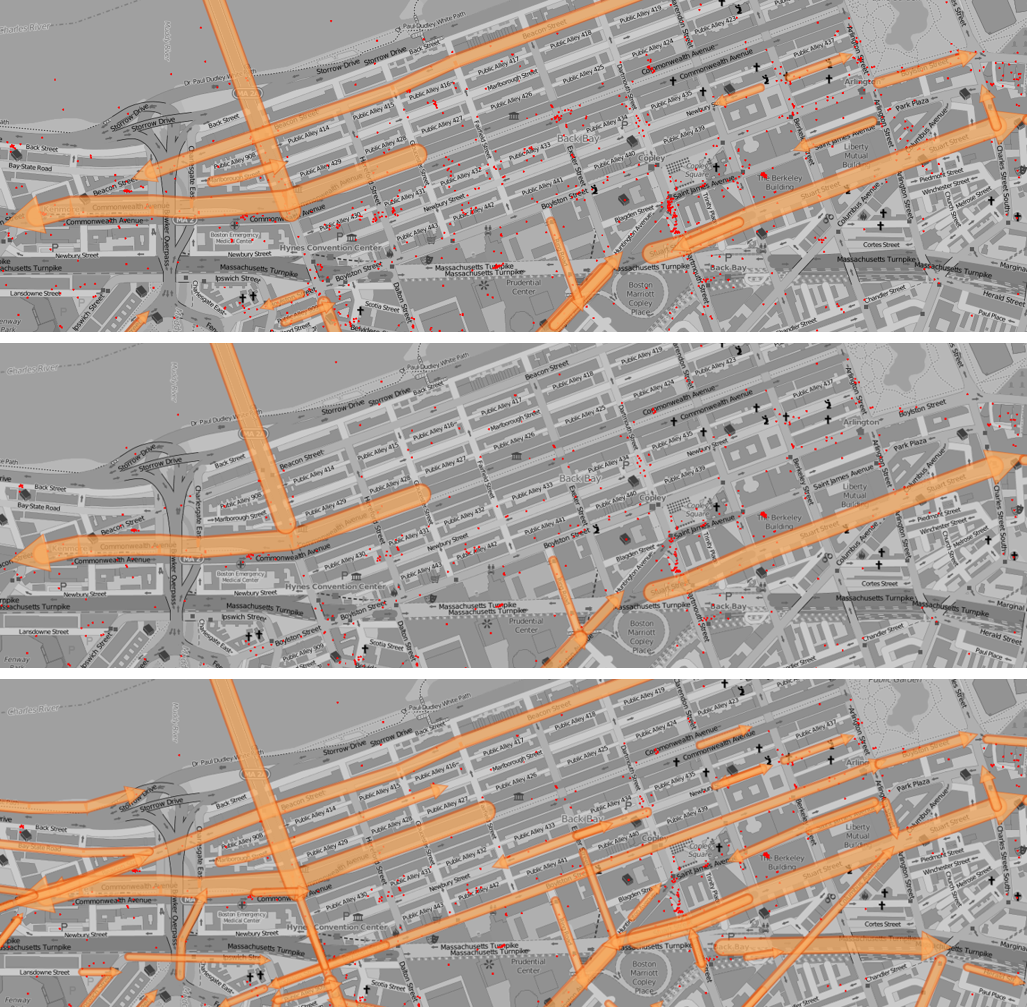
\includegraphics[width=1.0\linewidth]{clustering_level_v4}
	\caption{Clustering results depending on two parameters: $\epsilon$ and $MinLns$.
	Top ($\epsilon=25$, $MinLns=3$) is optimal.
	Center ($\epsilon=25$, $MinLns=4$) shows less number of trajectory clusters. Bottom ($\epsilon=30$, $MinLns=2$) shows more.
	}
	\label{fig:clustering_level}
	%\vspace{-0.4cm}
\end{figure}

%\subsection{Allow Customized Area Selection for Regional Trajectory Analysis}
%\subsection{Interaction}
%
%The system allows user to filter and display clusters related to a user select area. This feature allows user to select a specific polygonal area of interest and find trajectory clusters based on the trajectories that go through, go into or go out of that area.
%
%By implementing a mouse listener in Java, mouse movement and clicks can be tracked to both visualize and calculate the area has been chosen. Then each trajectory's joint points are tested to see if it lies within the selected area. If so, the trajectory is included in the selected trajectories. If a user chooses to calculate trajectory clusters under the selected area mode, the selected trajectories will be used to perform the clustering calculation. 

\begin{figure}[hbt]
	\centering
	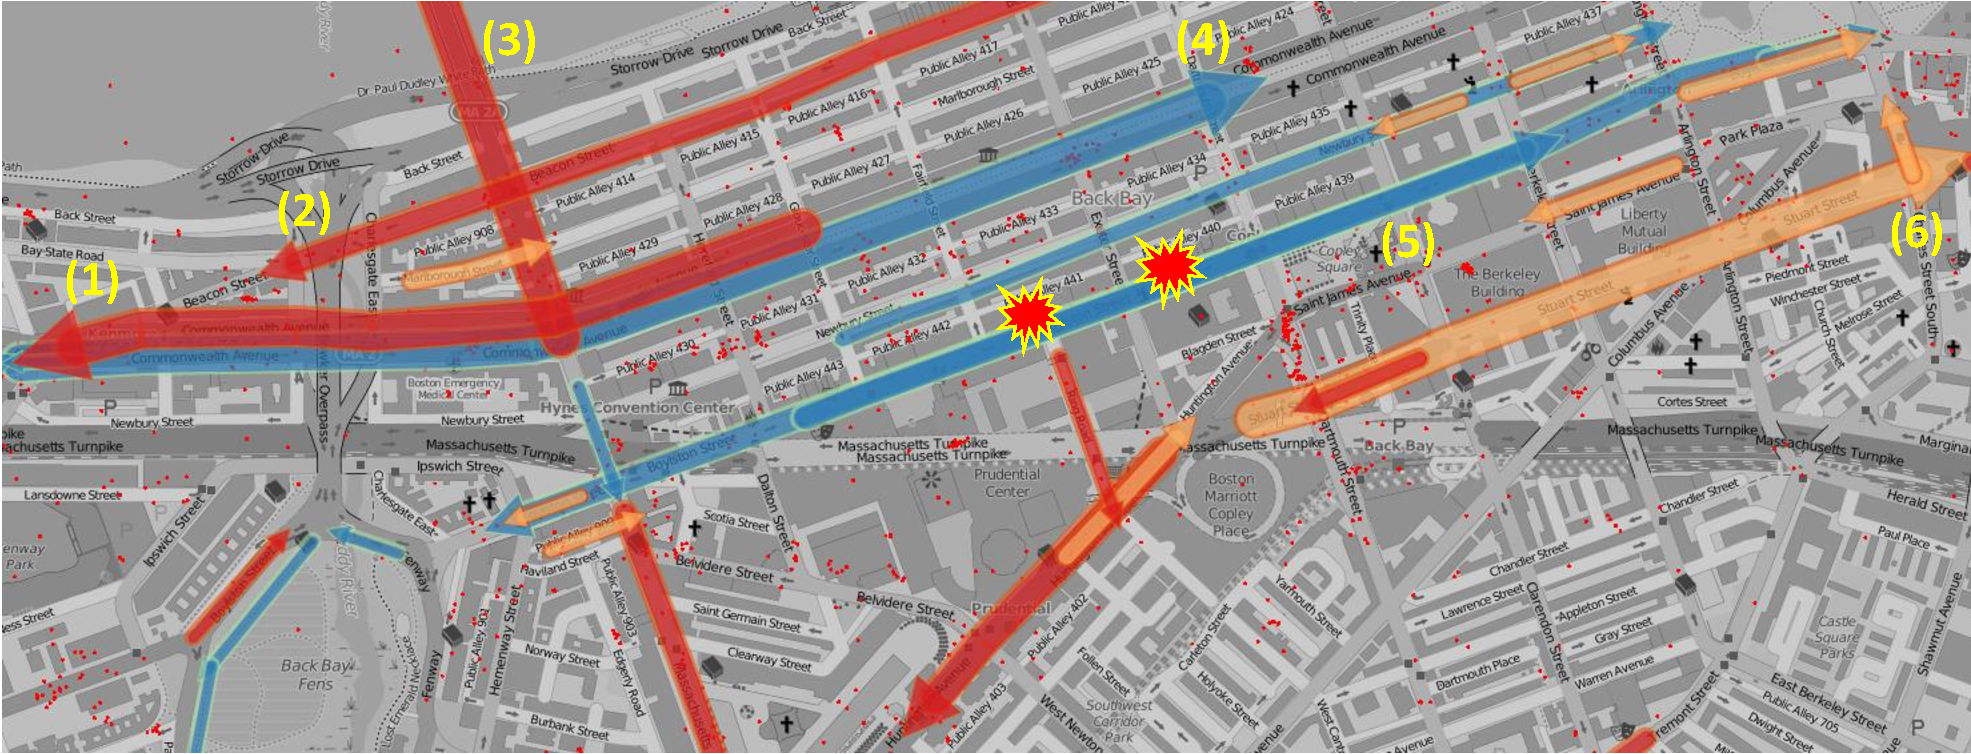
\includegraphics[width=1.0\linewidth]{abnormal_movements_v4}
	\caption{
	The trajectories (red and orange) shows the human movement patterns around the finish line at the Boston Marathon 2013 during 2 hours after the explosions.
	The trajectories (blue) represent the movements for the normal situation (the same time period of the same event in 2014).
	The two markers indicate the locations of the two explosions.
	}
	\label{fig:abnormal_movements}
	%\vspace{-0.4cm}
\end{figure}

\subsubsection{Visualization of Abnormal Movements}
\label{sec:visualization_abnormal}
Our analytics model identifies abnormal representative trajectories from target ones by comparing with normal ones as described in Section~\ref{sec:abnormal_movement_detection}.
We define target outliers are the abnormal representative trajectories and target normal trajectories are the rest of the target representative trajectories; the target normal trajectories are close to the normal representative trajectories.
We visualize the three different types of representative trajectories: target outlier, target normal, and normal using a similar visual encoding scheme described in the previous section.
We use different colors to distinguish between the different types: target outlier with red, target normal with orange, and normal with blue as shown in Figure~\ref{fig:abnormal_movements}.
%Figure~\ref{fig:abnormal_movements} shows an example case.
We can see that the trajectories (1), (2), and (3) are close to the normal trajectory (4), but they head toward the opposite direction.
Those are, therefore, classified as outliers.
The trajectory (6) is not classified as an outlier, because it is close to the normal trajectory (5) and also has the same direction.
We also provide an option to turn on/off each type to focus on a specific type.





\section{Improving Analysis using Multi-Context Information}
\label{sec:context}
In this section we describe our design goals of usage of each context.
We describe how we extract the context from multiple data sources.
Also, we show how the context is visually incorporated into the system.

\subsection{Keyword Extraction and Visualization}
%Trajectory clusters indicate common movements. 
%Those who move similarly and stay in the neighborhood at the same time period may experience common situations.
Analyzing the spatial behaviors alone is limited in achieving situational awareness of local events\textemdash they cannot answer why people move and what situations occur.
To address this  challenge, we extract keywords from the tweets used to generate a trajectory cluster and also those located close to the cluster, because such Tweets can contain common topics indicating an event occurring around a similar mobility.
Then we display the extracted keywords for providing additional insights into the event and the mobility patterns.

%\textbf{Keyword extraction:}
We select a set of Tweets that constitute sub-trajectories belonging to a cluster and are located within a specific distance to the representative trajectory of the cluster.
In this work, the default value of the distance threshold is set to 200 meters.
Then, we extract keywords from the text of the selected Tweets.
We calculate the frequencies of each word in the aggregate text and select top keywords based on the frequencies.
%The number of selected keywords depends on the number of selected tweets (maximum: 15 and minimum: 2).

%\textbf{Keyword visualization:} 
To display the extracted keywords, we utilize \textquoteleft tag cloud\textquoteright visualization.
Tag clouds have been used to represent a most frequent or important words in order to summarize text collections~\cite{Viegas:2008:Timelines}.
Also, tag clouds can be exploited for analytics tasks, such as topic-based document navigation and labeling geographical points of interest~\cite{Thom:2012:SAD,Luboschik:2008:Particle}.
In this work, we display the keywords along their corresponding representative trajectory without overlapping.
%Once the users hover a mouse pointer over a representative trajectory, it becomes darker and its keywords appear to avoid visual clutter.
The font size of each keyword encodes the frequency to show the popularity of the keyword.
Figure~\ref{fig:keyword_photo} (top) shows an example of showing extracted keywords display along the center trajectory. 
%The details on data will be explained in Section~\ref{sec:boston_marathon}.
%In case of overlapping trajectories, the shorter or thinner one under the mouse pointer will be selected. 
%The users can browse over the distributed trajectories to see if they have important keywords.

%~\cite{Nabo:2014:Annotating}
%In this work, we use tweets with geo-location, one of popular microblog services, which provide textual information, and geo-tagged photographs from photo sharing social network services (i.e., Instagram) and geo-tagged Tweets containing photographs provide image information.
\begin{figure}[htb]
	\centering
	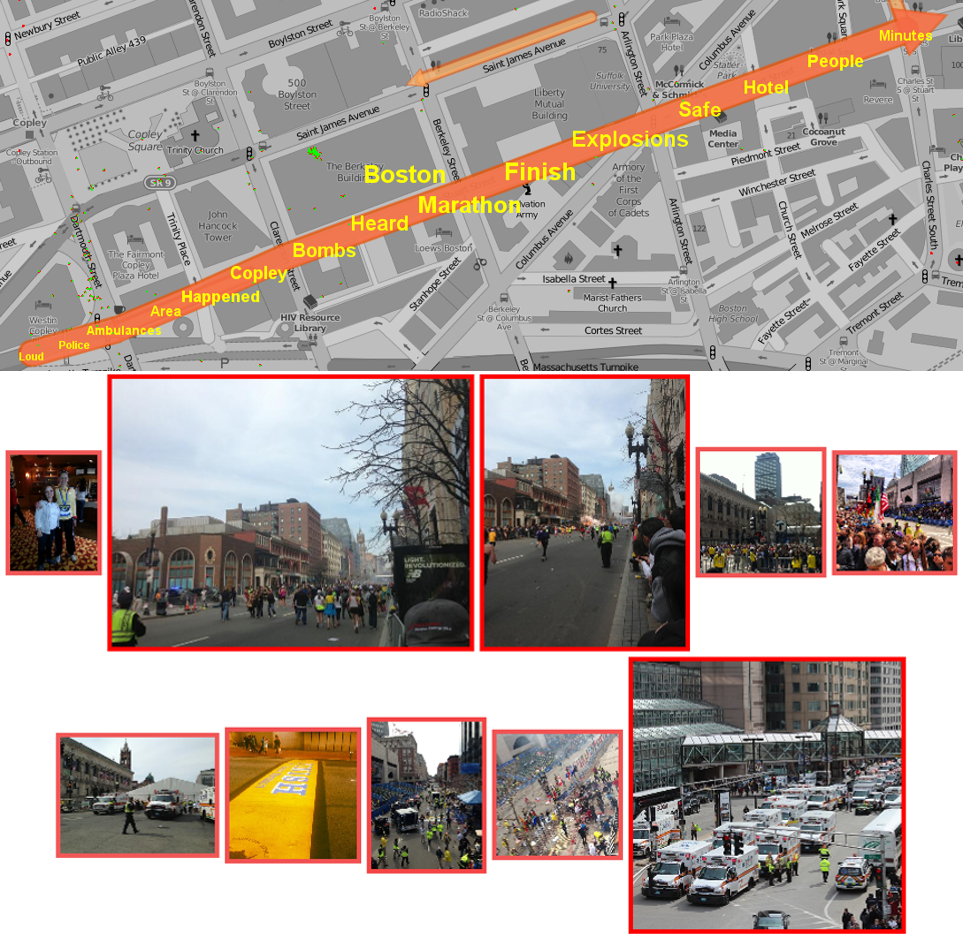
\includegraphics[width=1.0\linewidth]{keyword_photo_v2}
	\caption{
The extracted keywords along the trajectory close to the explosion locations show a strong relationship to the explosions (top).
The chronologically displayed photos (bottom) extracted from the same trajectory show the scenes of evolving situations.
}
	\label{fig:keyword_photo}
	%\vspace{-0.4cm}
\end{figure}

%\subsection{Improving situational awareness by shared photo, live public cameras, and news media}
\subsection{Additional Context Information}
For additional context, we utilize shared photos, public web camera videos, and news media related to each representative trajectory.
These data sources provide additional channels of information to users; thereby, providing a more comprehensive situational awareness for any emerging situation. 
%This context provide additional channels of information.
%Therefore, visualizations of the context can provide a more comprehensive view and improve movement analysis

\textbf{Shared photos:}
Right after people take photos, they can post the photos to LBSNs with their smartphones.
%A huge number of tweets include photos.
For example, we collected more than 230 of Tweets with photos were generated within the first 5 hours after the explosions at the Boston Marathon in 2013.
%1129 tweets with photos were generated during about 24 hours after the explosions at the Boston Marathon. 
The photos allow first responders and emergency managers to obtain a better situational awareness of what is happening on the site during a crisis.

In our system, we first select the Tweets in the same manner as for keyword extraction.
we identify Tweets with photos from the selected tweets for each trajectory cluster; tweets with photos contain photo links in a particular format.
Images are retrieved from links within Tweets and displayed chronologically in a separate window (e.g., as shown in Figure~\ref{fig:keyword_photo}).
%Then we extract the photo links and retrieve photos.
%These photos are chronologically displayed in a separate window to provide their temporal attributes.
Photo sizes correspond to relative differences in their sharing count (sum of retweets and replies)~\cite{Dork:2010:Visual}.
When a photo is selected, the location of the photo's Tweet is highlighted on the map.

\textbf{Public live web camera videos:}
%Even though there are quite a few public live web camera videos available online, use of implicit streaming data have a strong possibility to improve the temporal understanding of the situation at the site~\cite{Bergstrand:2011:VRT}.
We utilize public webcam video feeds to allow the emergency managers to obtain a better situational awareness of an emerging crises situation~\cite{Bergstrand:2011:VRT}.
In our system, we mark available camera locations on the map with pre-loaded camera location data~\cite{Purdue:2014:Webcam}.
Once users click on one of the web cameras icons on the map, the live streaming feed or most recent snapshots are provided (e.g., as shown in Figure~\ref{fig:purdue_shooting}).

\textbf{News media:}
%Sometimes information in social media provided by the public can be insufficient and inaccurate.
%However, news media reports from major news agencies are generally more abundant and accurate than one from the public.
We augment the information provided by the public in social media with news media reports from major news agencies.
News media reports related to the context of movements can provide more reliable information.
We search news reports with extracted keywords from nearby Tweets for each cluster using the Google search APIs.
The results, including titles, summaries and links of each news report, are displayed in a separate window.

\begin{figure}[htb]
	\centering
	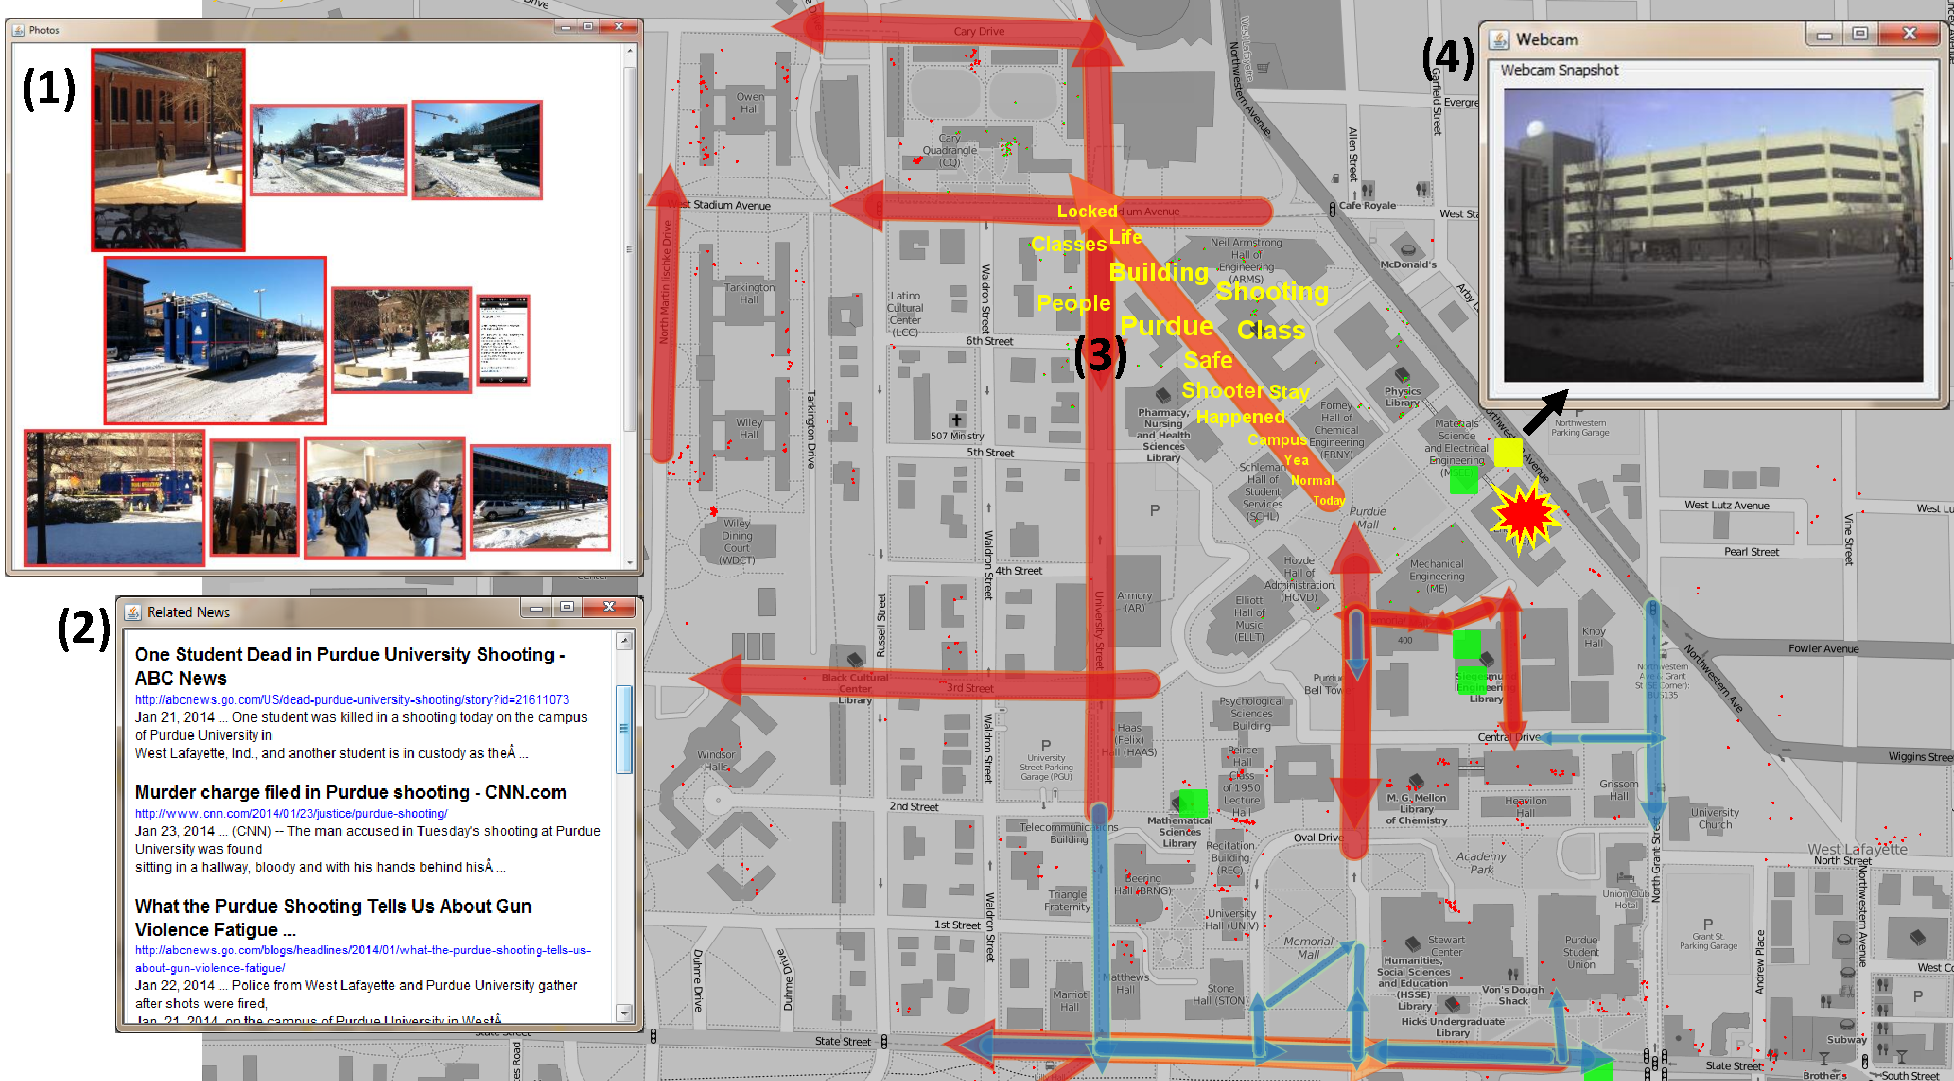
\includegraphics[width=1.0\linewidth]{purdue_shooting_v2}
	\caption{	
	The trajectories (red and orange) shows the human movements around the campus during 2 hours after the shooting.
	The normal trajectories (blue) extracted from the same time period on normal day.
	Photos (1), News reports (2), Keywords (3), and Webcam videos (4).
	The green rectangles indicate the locations of the web cameras around the campus. The yellow one is the selected camera.
	The marker indicate the building where the accident occurred.
	}
	\label{fig:purdue_shooting}
	%\vspace{-0.4cm}
\end{figure}
\section{Case Study}
In this section we demonstrate how our analytics model can assist emergency managers in discovering common/anomalous human movement patterns during crisis events, and how our visual analytics system improves movement analysis for disaster management personnel.

\subsection{Boston Marathon Explosion}
\label{sec:boston_marathon}

Boston Marathon is an annual marathon held in Greater Boston and one of the world's best-known athletic events.
On April 15, 2013, two bombs exploded near the finish line during the Boston Marathon at 2:49 pm EDT.
Figure~\ref{fig:abnormal_movements} shows two markers that indicate the locations of explosions.
%Three spectators were killed and about 260 people were injured in the bombings.
The trajectories in Figure~\ref{fig:abnormal_movements} show the movement patterns at the Boston Marathon, where the orange colored trajectories show the movements during the Boston Marathon bombing using Twitter data for the 2 hours after the explosions
The blue colored trajectories represent the normal movements using the data from next years' Boston Marathon event (we use next year's data for illustrative purposes instead of the previous year's data due to the unavailability of data for the previous year in our database).
The system utilizes these two trajectories in order to compute the abnormal trajectories (shown in red). 
%; we use the same time period of the same event in 2014.
The target trajectories (shown in orange) show that people were dispersed from the locations of the explosions and did not use the road where the accidents occurred.
Also, the outlier trajectories 1, 2, and 3 in Figure~\ref{fig:abnormal_movements} show that participants and spectators moved in the opposite direction of the finish line or crossed the bridge in order to get away from the location of impact.
Furthermore, Figure~\ref{fig:keyword_photo} (top) shows the keywords and photos extracted along the trajectory labeled 6 in Figure~\ref{fig:abnormal_movements} (note that the the photos chronologically displayed in the system).
Since the trajectory is close to the explosion locations, the extracted keywords along the trajectory show a strong relationship to the accident.
%Users can gain additional insights from the real scene photos which are chronologically ordered.
%The second and third photos in the first row show the exploding situations and the photos in the second row show the scenes after the explosions.
The system can thus enable first responders and law enforcement to detect anomalous movements and maintain a situational awareness of an emerging situation in their areas of responsibility. 

%\subsection{Ebola}
%\subsection{Hurricane Sandy}
\subsection{Purdue University Shooting}
On Tuesday, Jan 21st 2014, a shooting occurred inside one of the buildings of Purdue University, Indiana (shown by the marker in Figure~\ref{fig:purdue_shooting}).
Figure~\ref{fig:purdue_shooting} shows the movement patterns of people around the campus during 2 hours after the incident, where red colored trajectories show anomalous behavior, and orange colored trajectories show the movements during the 2 hours after the incident.
We compare the movements to the normal movements (blue) extracted from the same time period on another Tuesday.
We can observe anomalous behavior from the results where people moved to the left or upper-left regions.  Upon further investigation, we find that these locations house student residence halls.
Only a few people moved around the site of the incident, because of a lock down order given by the police.
In Figure~\ref{fig:purdue_shooting}, the photos (1) provide a visual context extracted from nearby Tweets of the trajectory (i.e., the scenes around the area and inside buildings).
The keywords (3) extracted from the selected trajectory convey more information describing the accident.
The news reports (2) extracted using the keywords along the tracectory (3) allow users to get more detailed information about the event.
Finally, the video feed (4) enables users to monitor the region in real time. 
Emergency managers can thus utilize social media as another input information source to maintain a situational awareness using our system.
\section{Summary}
We presented a trajectory-based visual analytics system, making it possible to: 1) generate trajectories using geo-tagged Tweets, 2) discover human common movement patterns, 3) detect abnormal movements, and 4) improve human movement analysis using semantic context available from multiple online media sources.
In order to find common movements, we utilize an enhanced partition-based clustering model that allows to extract similar portion of movements.
We proposed a classification model using human expert interaction to identify abnormal movements.
We described how we effectively extract and utilize relevant context, such as keywords extracted from Tweet text, shared photos, web camera videos, and news media for providing a better understanding of spatial movement behaviors.
We demonstrated the usage and effectiveness of our system for human movement analysis in abnormal situations by case studies.
%\section{Future Work}
%For future work, since we still have visual clutter issues, we plan to investigate solutions to reduce the clutter issues.
%In addition, we will request feedback from first responders and emergency managers for the usability and effectiveness of our system.

\chapter{Future Work}

We have presented preliminary results of visual spatiotemporal social media data analytics techniques for detection and examination of abnormal events, spatial decision support in crisis management, and anomalous human movement analysis.
%Thus far, the proposed techniques can be utilized in real-time or post-event analysis.
In emergency management and response, it is important to not only analyze what happened in the past and what is occurring in the present, but also predict what might arise in the future.
This can be done by using historical data and relevant context information to model and extrapolate future situations.
It is useful to know how current situations may change or when and where new situations may arise in the future.
This allows the emergency response to be more proactive instead of passive.
Although automated techniques are useful, user-guided controls can be applied to enhance the techniques.
This is because the accuracy is not guaranteed and unexpected situations should be taken into account.
In this context, as future work, we plan to develop predictive and interactive analytics techniques based on spatiotemporal social media data for integrating visual analytics approaches with automated data analysis models for predicting human movements.
The following sections describe in detail our plan of future study and a time line scheduled.

\section{Design of a Prediction Model using Historical Trajectory}
\label{sec:prediction_model}

Research on predicting human movements has attracted a lot of attention in recent years~\cite{Cho:2011:FAM,Jiang:2009:Ranking,Lin:2013:Predicting}.
The existing techniques have mainly focused on finding the next place of an individual based on the observations of his or her past movement patterns or frequent behaviors of similar users~\cite{Asahara:2011:PMP,Gambs:2012:NPP}.
In this work, we will focus on predicting overall flow of group movements.
We plan to design a model for predictive Vector Fields (VFs) based on spatiotemporal social media data, which is motivated by wind vector field maps.
An example of wind vector field map is shown in Figure~\ref{fig:wind}.
\begin{figure}[th]
	\centering
	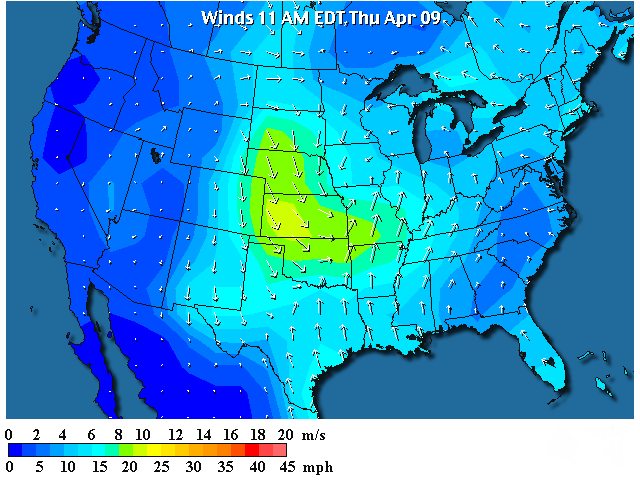
\includegraphics[width=0.8\linewidth]{wind_vector_field}
	\caption{Wind vector field map over the US~\cite{Weather:2015:Wind}.}
	\label{fig:wind}
\end{figure}

\textbf{Vector Field Generation:} 
The planned process of trajectory-based VF generation is the following:
%1) Generating trajectories for a specific time frame on a 2D space, 
%2) Dividing the trajectory space into sub-spaces on a grid, 
%3) For each cell, transforming the trajectories passing through the cell to vectors and calculating the sum of the vectors, and 
%4) Generating VFs using the sum vectors of each cell for the movements within the specific time frame.
\begin{enumerate}[label={(\arabic*)}]
	\item Generating trajectories of a specific time frame on a 2D space.
	\item Dividing the space of trajectories into sub-spaces on a grid.
	\item For each cell, transforming the trajectories passing through the cell into vectors and calculating the sum of the vectors.
	\item Generating vector fields using the sum vectors of each cell for visualizing the movement flow within a specific time frame.
\end{enumerate}
An initial result is shown in Figure~\ref{fig:vector_field} where the sample trajectories were generated around around the finish line at the Boston Marathon 2013 during 12 hours after the explosions.

\textbf{Vector Field Prediction:} 
The planned process of the future VFs prediction is the following:
\begin{enumerate}[label={(\arabic*)}]
	\item Creating a series of VFs for a certain past period of time frames,
	\item Extracting a series of vectors from the cells with a same coordinate from the series of VFs,
	\item Generating two time series, directions and magnitudes, of the series of vectors,
	\item Applying a temporal prediction method to the two time series for predicting the direction and the magnitude of the future vector of the coordinate, and
	\item Repeating the same procedure on each coordinate to create the future VFs.
\end{enumerate}
Figure~\ref{fig:vector_prediction} shows the overall procedure of our vector field prediction.

However, the VFs generated by traditional sum vectors have a limitation in representing flow of movements in specific cases.
For example, if there are two same size vectors pointing in opposite directions in a cell, the sum vector becomes a zero vector.
To mitigate this drawback, we will extract multiple dominant vectors based on the distribution of the vectors in a cell.
For temporal prediction methods of the time series, if the time series exhibit regular patterns (e.g., daily, weekly, monthly), the STL which is described in Section~\ref{subsec:filtering} will be a promising prediction method.
Also, our prediction model can be utilized to detect unusual movement flow in real-time by comparing actual real-time flow to the predicted one.

%Also, we will evaluate and improve our prediction model by using our about three years data.
%The cell is divided into the same number of sub-cells.
%The multiple dominant vectors are assigned to the sub-cells.

\begin{figure}[t]
	\centering
	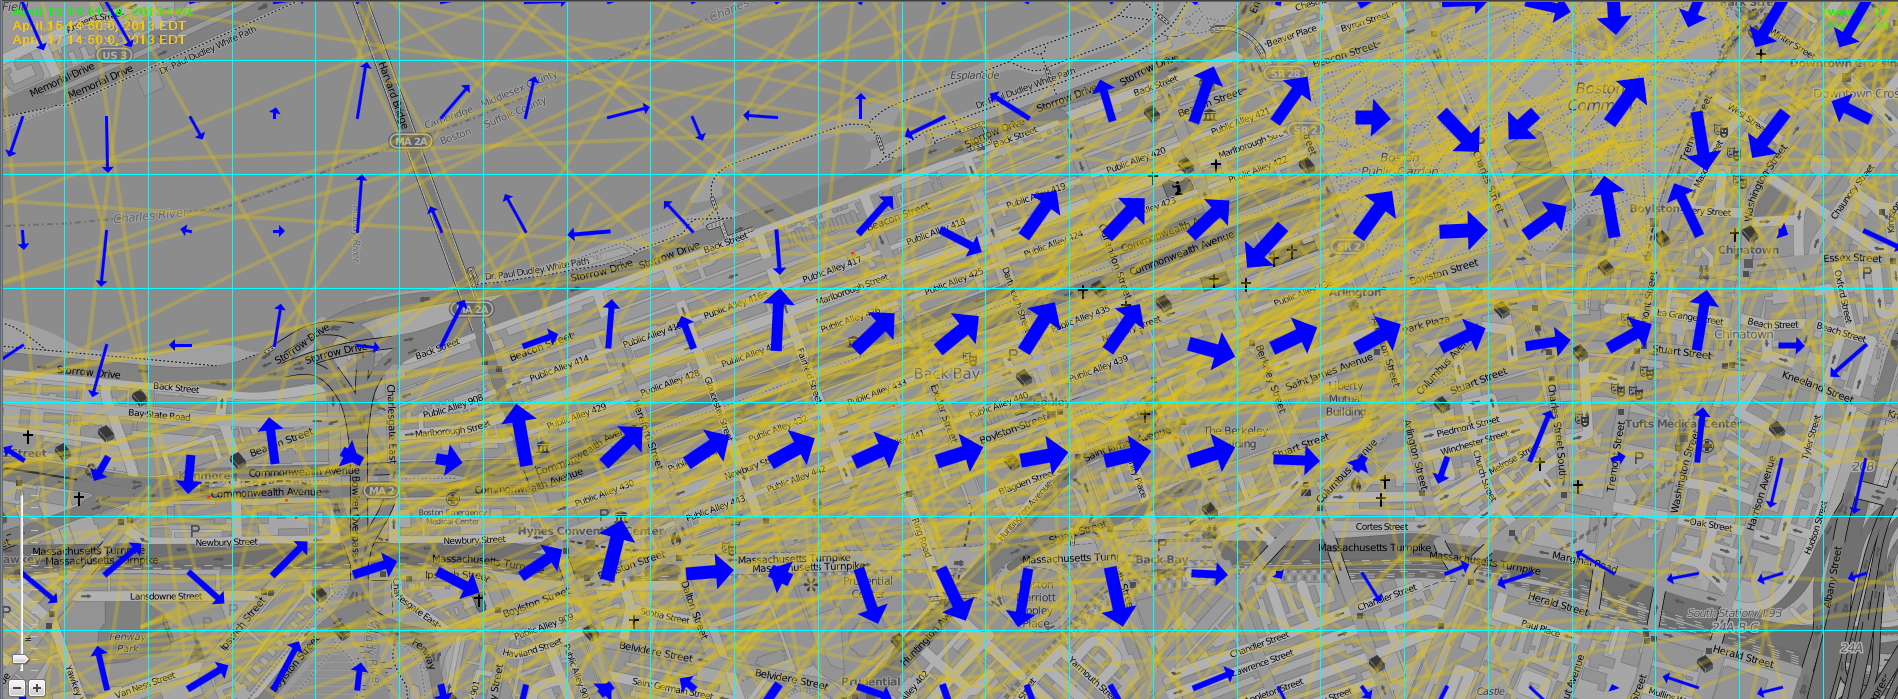
\includegraphics[width=1.0\linewidth]{CountasThicknessLengthasLength2}
	\caption{Initial results: vector field based on a trajectory space.}
	\label{fig:vector_field}
\end{figure}

\begin{figure}[t]
	\centering
	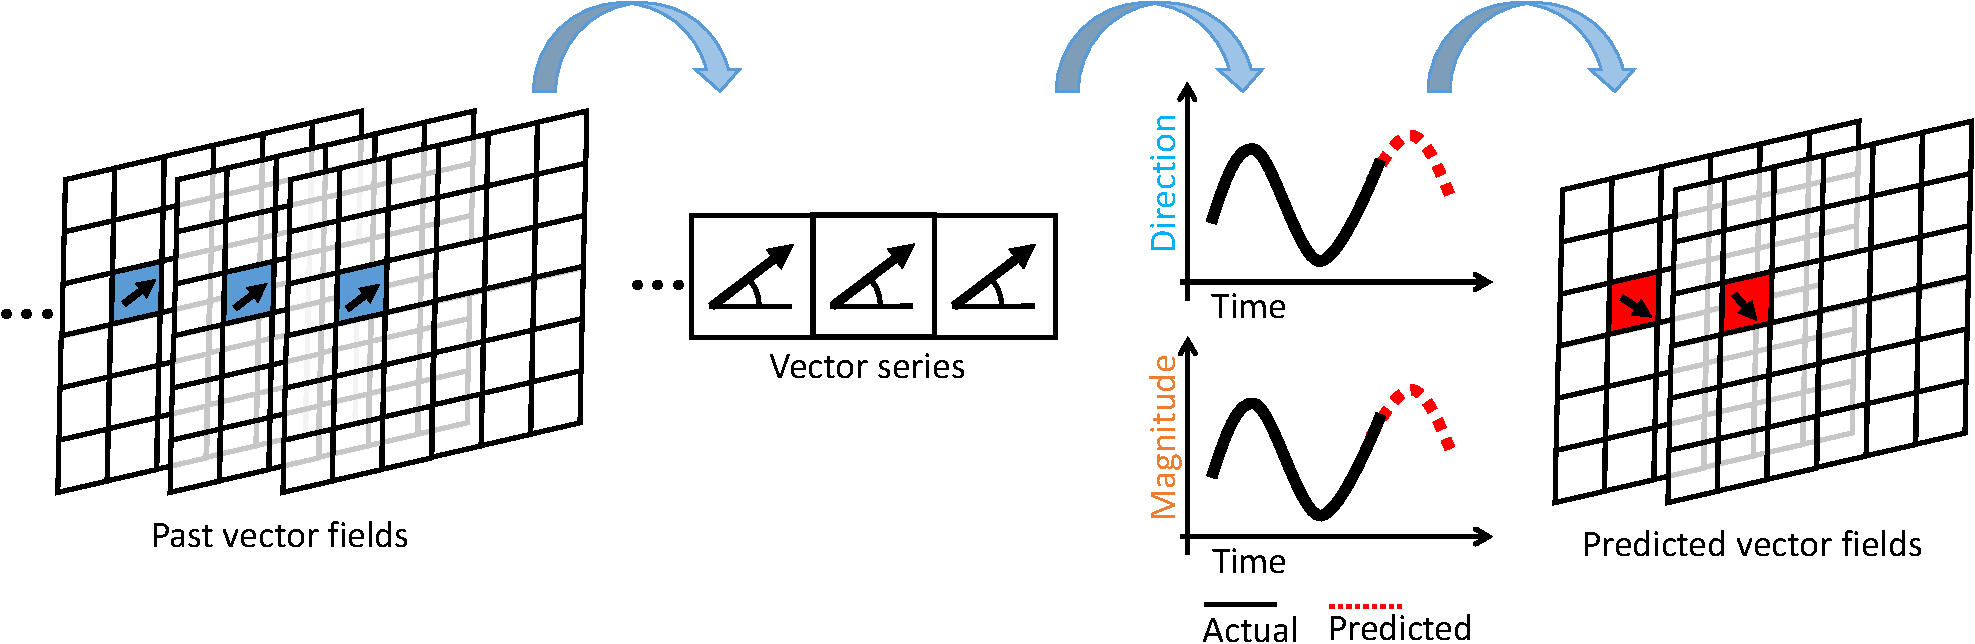
\includegraphics[width=1.0\linewidth]{vector_field_prediction}
	\caption{The process of vector field prediction}
	\label{fig:vector_prediction}
	%\vspace{-0.4cm}
\end{figure}

\textbf{Interactive Visualization:} 
%After calculating the predictive VFs generated by using the proposed prediction model, 
We plan to develop a visualization technique based on Line Integral Convolution (LIC)~\cite{Cabral:1993:Imaging}, a texture synthesis technique for flow visualization, to represent flow of the VFs (human movements).
%LIC is a texture synthesis technique for flow visualization.
%where it takes vector fields and a white noise image, convolves them to exploit spatial correlation in the flow direction.
%This technique takes a vector field and a white noise image, and convolves them in order to get something very similar to the images above.
While traditional LIC shows the streamlines of the vector fields, the directions of the vectors are not represented in the space.
To address this limitation, variations of LIC have been proposed, such as Animating Line Integral Convolution (ALIC) and Oriented Line Integral Convolution (OLIC)~\cite{Wegenkittl:1997:Animating,Wegenkittl:1997:Fast}.
Figure~\ref{fig:wind_isaac} shows an example of LIC visualization.
We will investigate and develop a LIC-based visualization technique to effectively visualize trajectory data.
%We will apply and test both visualization techniques (ALIC and OLIC) on our dataset.
We will develop a visual analytics system that provides interaction with not only the visualization, but also the back-end prediction model.


\begin{figure}[t]
	\centering
	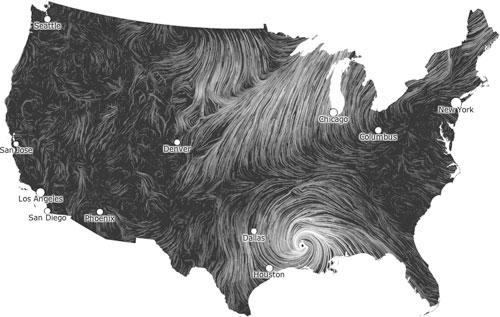
\includegraphics[width=0.8\linewidth]{wind_isaac_storm}
	\caption{LIC visualization showing wind flowing of Hurricane Isaac (September 2012) over the US
	%Zooming in south area (Bottom)
	~\cite{VW:2015:Windmap}.}
	\label{fig:wind_isaac}
	%\vspace{-0.4cm}
\end{figure}


\section{Integration of Context Information}

Human movements are affected by multiple factors including times of day (e.g., morning, evening), geographical features (e.g., school, bank), and specific events (e.g., sports game, festival).
%Researchers have worked on human movement mining using context information~\cite{Ying:2011:STM,Gonzalez:2008:UIH}.
Also, topics or keywords extracted from geo-tagged messages of a user can be utilized to infer the next place of the user.
In this context, we will investigate and design models using these context information to enhance the proposed prediction model described in Section~\ref{sec:prediction_model}.

Here is a possible virtual case study.
When an irregular event occurs, human movements may not conform to regular patterns.
For example, around a school campus, human mobility patterns on a sports game day evening may be different from the ones of a normal evening.
However, it will be able to pre-build a prediction model by leaning from past data of the same or similar events.
If so, we will detect the same or similar event on a specific day by the topic modeling described in Section~\ref{subsec:topic_extraction} and apply the pre-learned model for predicting the future movements.

\section{Evaluation}

We plan on performing evaluation of our prediction model using a large volume of historical data.
We have been collecting and storing Tweets on our database for more than three years since August, 2011.
To evaluate the prediction model, we will apply it to a variety of case studies including cases exhibiting regular patterns and abnormal patterns.
Also, we will evaluate our LIC-based visualization by comparing our technique with the existing visualization techniques for movement data (e.g., multiple poly-lines~\cite{Andrienko:2013:GroupMovement,Liao:2010:Anomaly} or series of arrows~\cite{Adrienko:2011:TrajAggregation,Andrienko:2007:Visual}).
%We will evaluate the prediction model based on datasets that exhibit either regular or irregular patterns in order to see robust 

%Also, we will evaluate and improve our prediction model by using our about three years data.

%\section{Interactive Visual Analytics System}

\section{Timeline}
%We schedule studies for the plans mentioned as future work in this proposal as following timeline:
Here is the expected schedule of the proposed future work as shown in Figure~\ref{fig:timeline}.
We will design a prediction model based on VFs using historical trajectory data from Summer 2015 and develop a LIC-based visualization technique during Fall 2015.
For enhancing our prediction model, we will start to develop a method by using context information in Fall 2015.
Finally, we will evaluate our prediction model and visualization technique in Spring 2016.

\begin{figure}[ht]
	\centering
	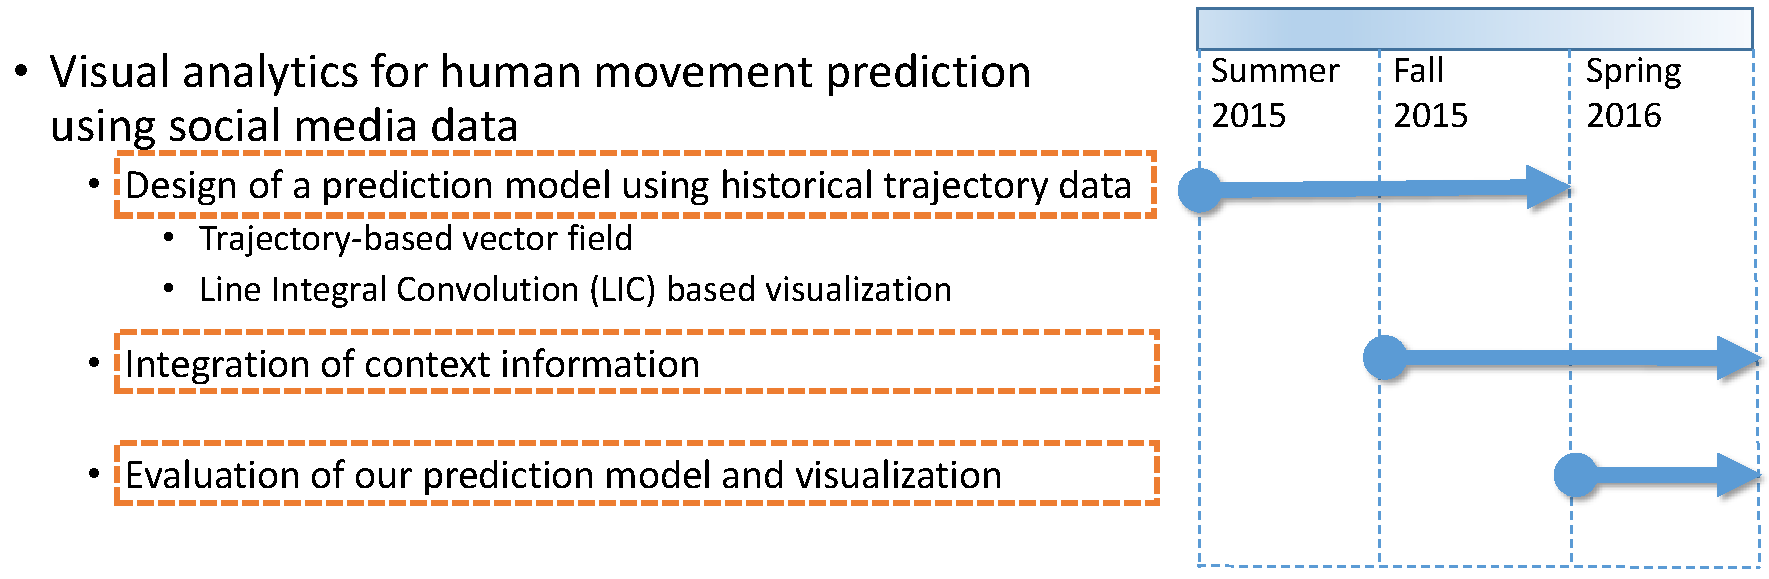
\includegraphics[width=1.0\linewidth]{timeline_v2}
	\caption{Proposed time line of future work}
	\label{fig:timeline}
\end{figure}






























% Put chapter \include commands here.

%\include{summary}

%\include{recommendations}

%
%  bibliography.tex     June 3, 2002     Mark Senn
%
%  This is the bibliography for a simple, example thesis.
%

\bibliography{ad_social_media,pb_sandy_comgraph,tra_trava,pre_trava}

% Use "\appendix" for one appendix or "\appendices" for more than one
% appendix.
\appendices
%\include{demo-citations}
%\include{demo-figures}
%\include{demo-mathematics}
%\include{demo-multicols}
%\include{demo-tables}
%\include{demo-text}

% A vita is optional for masters theses
% and required for doctoral dissertations.

%
%  vita.tex   2003.07.23  14:59:33   Mark Senn <mds@purdue.edu>
%
%  This is the vita for a simple, example thesis.
%
%  A vita is required only in a doctoral dissertation.
%

\begin{vita}
    [Put a brief autobiographical sketch here.]
\end{vita}

\end{document}
